\documentclass[12pt, a4paper]{report}

\usepackage{bm} % abych mohl psat tucne
\usepackage[czech]{babel} % cestina
\usepackage[T1]{fontenc}
\usepackage[utf8x]{inputenc}
\usepackage[unicode]{hyperref} % odkazy v pdf, www a na e-mail
\usepackage{graphicx} % obrazky
\usepackage{caption} % obrazky abych mohl udelat v popisku \\ ~
\usepackage{subcaption} % obrazky abych mohl udelat v popisku \\ ~
\usepackage{epstopdf} % obrazky
\usepackage{abraces, mathtools} % svorka zespoda
\usepackage{lmodern} % daji se pouzit \HUGE atd.
\linespread{1.10} % radkovani 1.3 odpovida radkovani 2



\usepackage[numbered,framed]{matlab-prettifier} %vkladani kodu matlabu
\lstset{style = Matlab-editor, basicstyle = \mlttfamily, escapechar = ", mlshowsectionrules = true,}

%------------------DRAFT----------------------------
\usepackage{draftwatermark}
\SetWatermarkLightness{0.95}
\SetWatermarkScale{1}
\SetWatermarkText{DRAFT}

%------------------LAYOUT----------------------------
\usepackage[top = 2.5 cm, bottom = 2.5 cm, left = 2.5 cm, right = 2.5 cm]{geometry} % geometrie stranky
\usepackage{longtable}% Pro dlouhy obsah, da se zalomit \pagebrek
\usepackage{fancyhdr}
\pagestyle{fancy}% Deffaultni nastaveni hlavicky a paticky
\setlength{\headheight}{16 pt}% Zvetsi hlavicku, aby to nedelalo warningy
\fancyhf{}
\lhead{\bfseries \leftmark}
\fancyfoot[R]{\thepage}
\fancyfoot[L]{Poslední úpravy: \today}

%****************************************************
\begin{document}

%
%--------TITULNI-STRANA------------------------------
\begin{titlepage}
\begin{center}
	\vspace*{\fill}
	\textbf{\Huge{Klasifikace a strojové učení}}\\
	\vspace*{\fill}
	\textbf{\large{\href{mailto:LBures@kky.zcu.cz}{Ing. Lukáš Bureš}}} \hfill \textbf{\large{Plzeň}}\\
	\textbf{\large{Katedra kybernetiky}} \hfill \textbf{\large{\today}}
\end{center}
\end{titlepage}


%--------OBSAH----------------------------------------
\setcounter{page}{1}
\pagenumbering{Roman}

\tableofcontents
\newpage

\listoffigures
\newpage

\listoftables
\newpage

\setcounter{page}{1}
\pagenumbering{arabic}

%--------SEKCE----------------------------------------


%------------UVOD--------------------------
\chapter{Předmluva}
\label{sec:Predmluva}

\par{Tento studijní materiál vznikl na Západočeské univerzitě v~Plzni, Fakultě aplikovaných věd, Katedře kybernetiky jako pomocný podklad pro předměty Zpracování digitalizovaného obrazu (KKY/ZDO) a Metody počítačového vidění (KKY/MPV) v~roce 2014.}

\par{CV je nejlepší, moderní atd.}

\par{Machine learning .}

\newpage












%----UVOD----------------------------------------------------------------------------------
\chapter{Úvod}
\label{sec:Uvod}









%----CO-JE-STROJOVE-UCENI-------------------------------------------------------------------
\section{Co je strojové učení?}
\label{sec:UvodCoJeStrojoveUceni}

\par{Pojem strojové učení nemá dodnes pevně danou definici, můžeme si ukázat několik pokusů o jeho definování
\begin{itemize}
	\item Arthur Samuel (1959). Strojové učení: \textit{Obor, který dává počítačům schopnost učit se bez toho, aby byly přímo naprogramovány.}
	\item Tom Mitchell (1998): Dobře definovaný problém strojového učení: \textit{Předpokladem je, že se počítačový program učí ze zkušeností \textbf{E} s respektováním úlohy \textbf{T} a s měřičem výkonu \textbf{P}, pokud se jeho výkon na úloze \textbf{T} měřený pomocí \textbf{P} zvyšuje se zkušeností \textbf{E}.}
\end{itemize}}

\par{Pokusme se jednotlivé části rozebrat na příkladu: Předpokládejme, že náš emailový klient sleduje, které email označíme nebo neoznačíme jako spam. Na základě tohoto rozhodnutí se náš emailový klient učí lépe rozpoznávat co je a co není spam. Nyní si můžeme položit otázku co z následujících tvrzení je úloha \textbf{T}?
\begin{enumerate}
	\item Klasifikace emailů jako spam nebo vyžádaný email.
	\item Sledování značek od uživatele, který email označil jako spam nebo vyžádaný email.
	\item Počet (nebo poměr) emailů, které byly správně klasifikovány jako spam nebo vyžádaný email.
	\item Nic z výše uvedeného - není to problém strojového učení.
\end{enumerate}
Pokud si rozebereme jednotlivé body výše, tak bod jedna je definice úlohy \textbf{T}, dále bod dva je zkušenost \textbf{E} a třetí bod je náš měřič výkonu \textbf{P}.}

\par{Existuje několik rozdílných typů učících se algoritmů. Hlavní dva typy se nazývají
\begin{itemize}
	\item učení s učitelem a
	\item učení bez učitele.
\end{itemize}}
\newpage
















%----UCENI-S-UCITELEM-----------------------------------------------------------------
\section{Učení s učitelem}
\label{sec:UvodUceniSUcitelem}

\par{\textbf{Učení s učitelem} je metoda strojového učení pro učení funkce z trénovacích dat. Trénovací data sestávají ze dvojic vstupních objektů (typicky vektorů příznaků) a požadovaného výstupu. Výstup funkce může být spojitá hodnota (při regresi) anebo může předpovídat označení třídy vstupního objektu (při klasifikaci). Úloha algoritmu učení je předpovídat výstupní hodnotu funkce pro každý platný vstupní objekt poté, co zpracuje trénovací příklady (tj. dvojice vstup a požadovaný výstup). Aby to dokázal, musí algoritmus zobecnit prezentovaná data na nové situace (vstupy) \uv{smysluplným} způsobem. Analogická úloha v lidské a zvířecí psychologii se často nazývá učení konceptů.

\par{\textbf{Přetrénování} (anglicky \textit{overfitting}) je stav, kdy je systém příliš přizpůsoben množině trénovacích dat, ale nemá schopnost generalizace a selhává na testovací (validační) množině dat. To se může stát například při malém rozsahu trénovací množiny nebo pokud je systém příliš komplexní (například příliš mnoho skrytých neuronů v neuronové síti). Řešením je zvětšení trénovací množiny, snížení složitosti systému nebo různé techniky regularizace, zavedení omezení na parametry systému, které v důsledku snižuje složitost popisu naučené funkce, nebo předčasné ukončení (průběžné testování na validační množině a konec učení ve chvíli, kdy se chyba na této množině dostane do svého minima).}

\par{Při učení se používají trénovací data (nebo trénovací množina), testovací data a často validační data.}

\par{\textbf{Příklady algoritmů:} rozhodovací stromy, AdaBoost, náhodné rozhodovací lesy, metoda nejbližšího souseda, metoda K-nejbližších sousedů, lineární regrese, Bayesův klasifikátor, neuronové sítě, binární regrese, support vector machine (SVM), atd.}















%-----UCENI-BEZ-UCITELEM-----------------------------------------------------------------
\section{Učení bez učitele}
\label{sec:UvodUceniBezUcitele}

\par{\textbf{Příklady algoritmů:} BIRCH, hierarchické algoritmy, divizní algoritmy, K-means (MacQueen algoritmus), expectation-maximization (EM) algoritmus, atd.}

\newpage





















%----------------LINEARNI-REGRESE--------------------------
\section{Lineární regrese}
\label{sec:LinearniRegrese}

\par{Lineární regrese je matematická metoda používaná pro proložení souboru bodů v grafu přímkou. O bodech reprezentujících měřená data se předpokládá, že jejich $x$-ové souřadnice jsou přesné, zatímco $y$-nové souřadnice mohou být zatíženy náhodnou chybou, přičemž předpokládáme, že závislost $y$ na $x$ lze graficky vyjádřit přímkou. Pokud měřené body proložíme přímkou, tak při odečítání z grafu bude mezi $y$-novou hodnotou měřeného bodu a $y$-novou hodnotou ležící na přímce odchylka. Podstatou lineární regrese je nalezení takové přímky, aby součet druhých mocnin těchto odchylek byl co nejmenší. Lineární regresi lze zobecnit i pro prokládání jinou funkcí než přímkou.}










%------------------MOTIVACE--------------------------------
\subsection{Motivace}
\label{sec:LinearniRegreseMotivace}

\par{Jako motivaci můžeme použít příklad, kdy si budete chtít zakoupit byt v~Plzni, proto by bylo dobré znát, kolik zaplatíte za jakou podlahovou plochu, v ideálním případě pro všechny velikosti bytů. Nebo-li se snažíte predikovat cenu bytu v~závislosti na podlahové ploše. Na Obr. \ref{fig:cena_plocha} lze vidět vývoj ceny bytu v~závislosti na podlahové ploše.}

\begin{figure}[!ht]
	\centering
	%trim option's parameter order: left bottom right top
	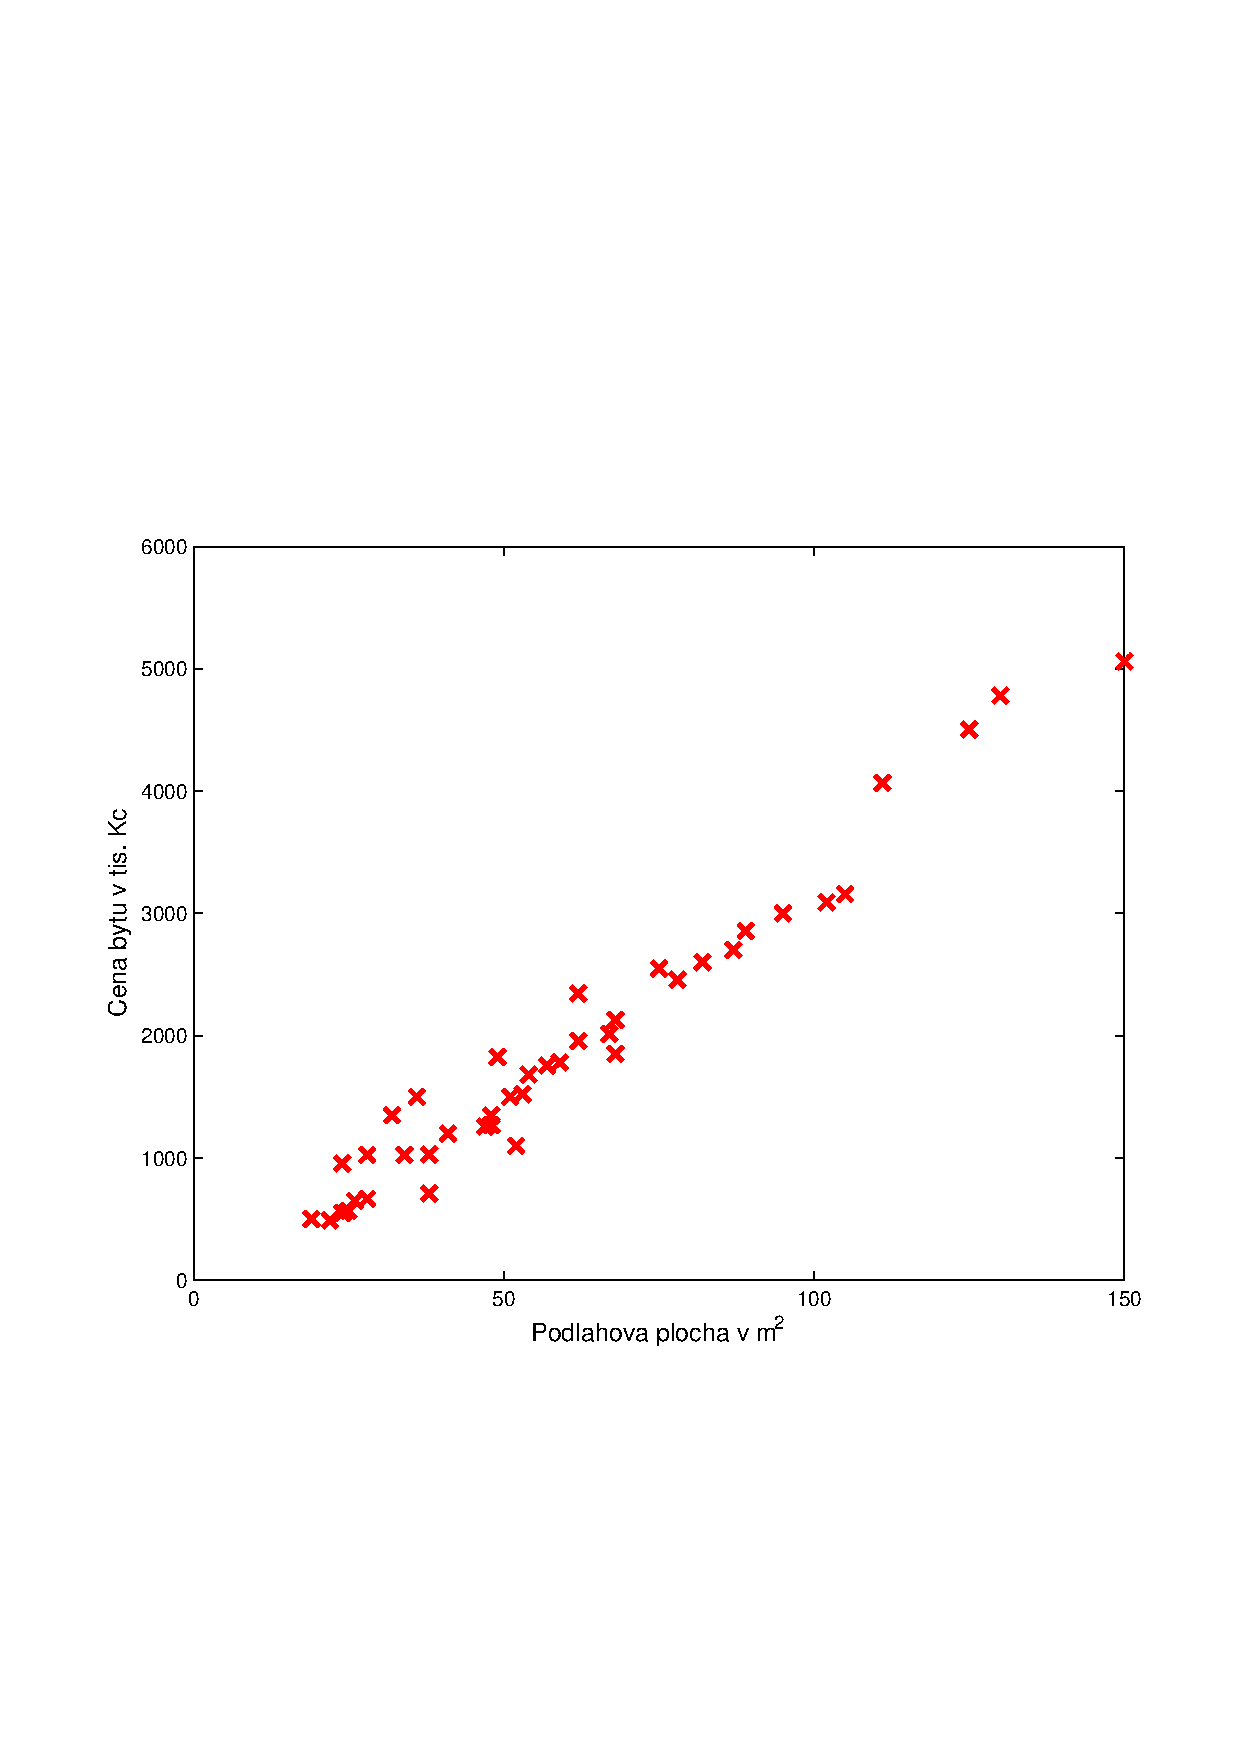
\includegraphics[scale = 0.5, trim = 3cm 7cm 3cm 9cm]{./Img/LinearniRegrese/cena_plocha.pdf}
	\caption{Vývoj ceny bytu v závislosti na podlahové ploše.}
	\label{fig:cena_plocha}
\end{figure}





%----------------UCENI-S-UCITELEM--------------------
\subsection{Učení s učitelem}
\label{sec:LinearniRegreseUceniSUcitelem}

\par{Učení s~učitelem (supervised learning) dává \uv{správnou odpověď} pro každý příklad z~množiny dat.}

\par{Problém regrese: Na základě reálného (spojitého) vstupu predikovat reálný (spojitý) výstup.}

\par{Problém klasifikace: Na základě diskrétního vstupu predikovat diskrétní výstup.}

\par{Více formálně v~případě učení s~učitelem potřebujeme množinu dat nazývanou trénovací množina. V~našem případě predikce ceny bytu máme trénovací množinu cen bytů a~k~nim odpovídající podlahovou plochu. Naším úkolem je naučit se z~těchto dat jak predikovat ceny bytů.}

\par{Nyní zavedeme notaci nechť $m$ je velikost trénovací sady, $x$ jsou \uv{vstupní} proměnné neboli příznaky a~$y$ jsou \uv{výstupní} proměnné neboli příznaky. Jeden trénovací vzorek budeme označovat jako $\left(\bm{x}, y \right)$ a~odpovídá jednomu řádku v~tabulce \ref{tab:vzorky}. Dále $\left( x^{\left( i \right)}, y^{\left( i \right)} \right)$ označuje $i$-tý trénovací vzorek.}

\begin{table}[!ht]
\centering
\begin{tabular}{c|c}
	{Velikost bytu v $m^2$ ($x$)} & {Cena bytu v tis. Kč ($y$)}\\
	\hline
	{19} & {500}\\
	{22} & {490}\\
	{25} & {568}\\
	{$\ldots$} & {$\ldots$}
\end{tabular}
\caption{Příklady trénovacích vzorků.}
\label{tab:vzorky}
\end{table}

\par{Trénovací množina, v~našem případě ceny bytů, je potřebná pro natrénování učícího se algoritmu, jehož výstupem je funkce (hypotézy), která se většinou označuje $h$. Účelem funkce (hypotézy) $h$ je ze vstupu $x$ (velikost bytu) odhadnout výstup $y$ (cena bytu). Tedy $h$ je funkce, která mapuje $x$ na $y$. Schéma je naznačeno na Obr. \ref{fig:schema}.}

\begin{figure}[!ht]
	\centering
	%trim option's parameter order: left bottom right top
	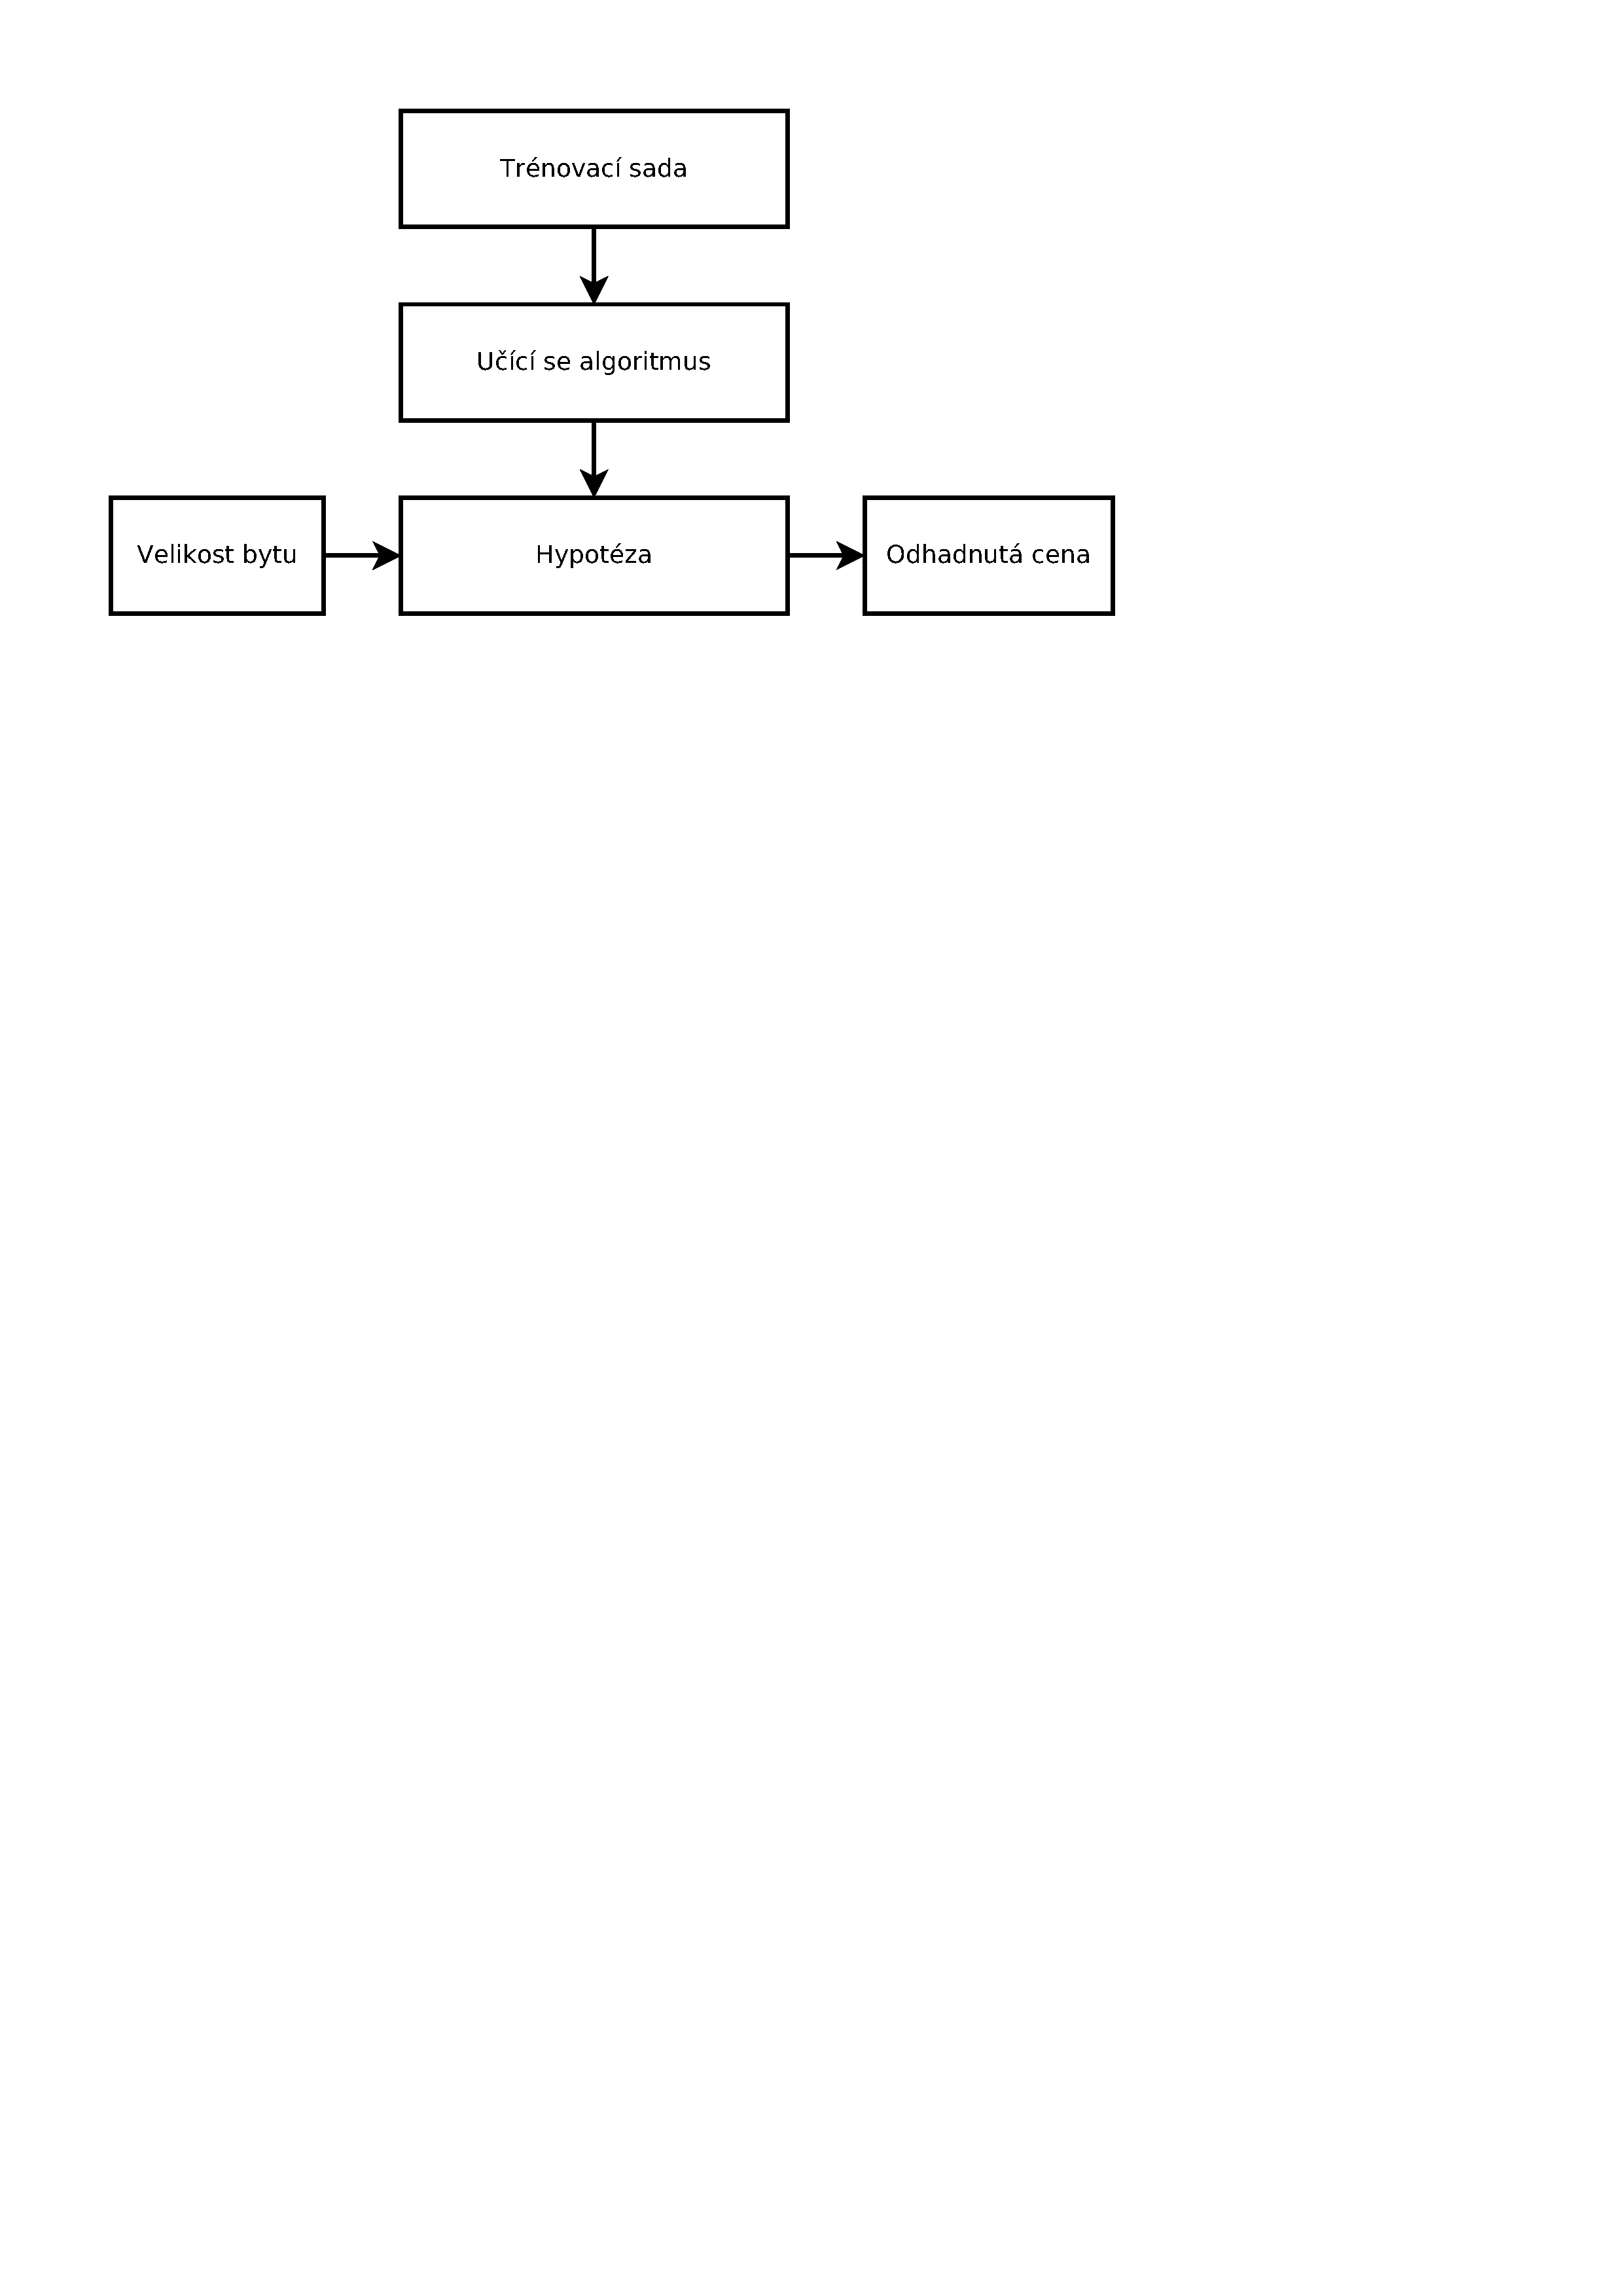
\includegraphics[scale = 0.5, trim = 3.5cm 42cm 14cm 2cm]{./Img/LinearniRegrese/schema.pdf}
	\caption{Schéma učení s učitelem.}
	\label{fig:schema}
\end{figure}

\par{Když navrhujeme učící se algoritmy, další věc kterou potřebujeme rozhodnout je jak budeme reprezentovat hypotézu $h$. V~našem motivačním příkladě si vystačíme s~hypotézou v~následujícím tvaru lineární funkce:
\begin{equation}
	h_{\bm{\Theta}} \left( x \right) = \vartheta_0 + \vartheta_1 x,
\end{equation}
zkráceně $h \left( x \right)$. Jedná se tedy o~lineární regresi s~jednou proměnnou. V~případě komplexnějšího učícího se algoritmu je nutné použít složitější nelineární model.}

\subsubsection*{Poznámka}
\par{$\vartheta$ je malá théta a $\Theta$ je velká théta.}

\newpage















%----------------ZTRATOVA-FUNKCE---------------------
\subsection{Ztrátová funkce}
\label{sec:LinearniRegreseZtratovaFunkce}

\par{Pro nejlepší napasování našeho lineárního modelu na trénovací data budeme potřebovat určit parametr $\vartheta_0$ a~$\vartheta_1$ v~naší hypotéze:
\begin{equation}
	h_{\bm{\Theta}} \left( x \right) = \vartheta_0 + \vartheta_1 x,
\end{equation}}

\par{Snažíme se zvolit parametry $\vartheta_0$ a $\vartheta_1$ tak, aby hypotéza $h_{\bm{\Theta}} \left( x \right)$ byla co nejblíže k $y$ pro naše trénovací vzorky $\left( x, y \right)$. Jinými slovy snažíme se minimalizovat kvadratickou chybu:

\begin{equation}
	\min_{\vartheta_0, \vartheta_1} \frac{1}{2m} \sum_{i = 1}^{m} \left( h_{\bm{\Theta}} \left( x^{\left( i \right)} \right) - y^{\left( i \right)} \right)^2,
\end{equation}
kde
\begin{equation}
	h_{\bm{\Theta}} \left( x^{\left( i \right)} \right) = \vartheta_0 + \vartheta_1 x^{\left( i \right)}.
	\label{eq:hProJednoDato}
\end{equation}
Přesněji označíme ztrátovou funkci:
\begin{equation}
	J \left( \vartheta_0, \vartheta_1 \right) = \frac{1}{2m} \sum_{i = 1}^{m} \left( h_{\bm{\Theta}} \left( x^{\left( i \right)} \right) - y^{\left( i \right)} \right)^2
\end{equation}
a minimalizujeme
\begin{equation}
	\min_{\vartheta_0, \vartheta_1} 	J \left( \vartheta_0, \vartheta_1 \right).
\end{equation}
Tato ztrátová funkce $J$ je také občas nazývána kvadratická chyba nebo ztrátová funkce kvadratické chyby.}

\par{Ztrátová funkce ve formě kvadratické chyby je nejčastěji používanou ztrátovou funkcí při řešení regresních problémů.}





\newpage








%----------------GRADIENT-DESCENT---------------------
\subsection{Gradientní algoritmus}
\label{sec:LinearniRegreseGradientDescent}

\par{V~kapitole \ref{sec:LinearniRegreseZtratovaFunkce} jsme definovali ztrátovou funkci $J$. V~této kapitole bude popsán gradientní algoritmus pro minimalizaci ztrátové funkce $J$. Gradientní algoritmus není omezen jen a~pouze na lineární regresi nalézá uplatnění v~optimalizaci a~v~dalších oblastech strojového učení.} 

\par{Máme ztrátovou funkci $J \left( \vartheta_0, \vartheta_1 \right)$ a~chtěli bychom jí minimalizovat. Proto zvolíme náhodně $\vartheta_0$ a~$\vartheta_1$, dále v~každé iteraci měníme hodnoty $\vartheta_0$ a~$\vartheta_1$, tak abychom redukovali $J \left( \vartheta_0, \vartheta_1 \right)$ dokud, v~nejlepším případě, nedokonvergujeme do globálního minima.}

\par{Obecně lze gradientní algoritmus použít na jakoukoliv ztrátovou funkci:
\begin{equation}
	J \left( \vartheta_0, \cdots, \vartheta_n \right)
\end{equation}
a snažíme se minimalizovat:
\begin{equation}
	\min_{\vartheta_0, \ldots, \vartheta_n} J \left( \vartheta_0, \ldots, \vartheta_n \right)
\end{equation}}

\par{Definice gradientního algoritmu: opakuj dokud není dosaženo konvergence
\begin{equation}
	\vartheta_j = \vartheta_j - \alpha \frac{\partial}{\partial \vartheta_j} J \left( \vartheta_0 , \vartheta_1 \right),
	\label{eq:gradDescentIter}
\end{equation}
pro $j = \{ 0, 1 \}$, pro náš příklad (lineární regrese jedné proměnné) v~sekci \ref{sec:LinearniRegreseMotivace}. V~rovnici \ref{eq:gradDescentIter} proměnná $\alpha$ určuje, jak velké kroky bude gradientní algoritmus dělat při hledání minima a~nazývá se rychlost učení. V~případě velké hodnoty $\alpha$ bude algoritmus postupovat velkými kroky, rychle, ale není zajištěna konvergence, jelikož se může stát, že algoritmus bude kroužit kolem minima, ale nedosáhne ho, nebo bude divergovat. V~případě malé hodnoty $\alpha$ bude algoritmus velice pomalý a~nemusí dosáhnout minima pro stanovený počet iterací. Gradientní algoritmus může konvergovat do lokálního minima v~případě, že je rychlost učení $\alpha$ konstantní. Proto se v~reálných aplikacích volí nejdříve větší $\alpha$, které se s~rostoucí hodnotou iterací nebo času zmenšuje.}

\subsubsection*{Poznámka}
\par{Pro implementaci: je nutné aktualizovat všechny $\Theta$ současně
\begin{eqnarray}
	&temp_0 &= \vartheta_0 - \alpha \frac{\partial}{\partial \vartheta_0} J \left( \vartheta_0 , \vartheta_1 \right),\\
	&temp_1 &= \vartheta_1 - \alpha \frac{\partial}{\partial \vartheta_1} J \left( \vartheta_0 , \vartheta_1 \right), \\
		&\vartheta_0 &= temp_0, \\
		&\vartheta_1 &= temp_1.
\end{eqnarray}}

\par{Nyní budeme aplikovat gradientní algoritmus na náš problém lineární regrese
\begin{equation}
	\frac{\partial}{\partial \vartheta_j} J \left( \vartheta_0, \vartheta_1 \right) = \frac{\partial}{\partial \vartheta_j} \cdot \frac{1}{2m} \sum_{i = 1}^{m} \left( h_{\bm{\Theta}} \left( x^{\left( i \right)} \right) - y^{\left( i \right)} \right)^2,
\end{equation}
po dosazení z~rovnice \ref{eq:hProJednoDato} dostáváme
\begin{equation}
	\frac{\partial}{\partial \vartheta_j} J \left( \vartheta_0, \vartheta_1 \right) = \frac{\partial}{\partial \vartheta_j} \cdot \frac{1}{2m} \sum_{i = 1}^{m} \left( \vartheta_0 + \vartheta_1  x^{\left( i \right)} - y^{\left( i \right)} \right)^2,
\end{equation}
po zderivování podle jednotlivých parametrů $\Theta$ získáme
\begin{eqnarray}
	\frac{\partial}{\partial \vartheta_0} &J \left( \vartheta_0, \vartheta_1 \right) &= \frac{1}{m} \sum_{i = 1}^{m} \left( h_{\bm{\Theta}} \left( x^{\left( i \right)} \right) - y^{\left( i \right)} \right),\\
	\frac{\partial}{\partial \vartheta_1} &J \left( \vartheta_0, \vartheta_1 \right) &= \frac{1}{m} \sum_{i = 1}^{m} \left( h_{\bm{\Theta}} \left( x^{\left( i \right)} \right) - y^{\left( i \right)} \right) x^{\left( i \right)}.
\end{eqnarray}}

\par{Výsledný konkrétní tvar rovnice \ref{eq:gradDescentIter} pro $\vartheta_0$ a $\vartheta_1$
\begin{eqnarray}
		&\vartheta_0 &= \vartheta_0 - \alpha \frac{1}{m} \sum_{i = 1}^{m} \left( h_{\bm{\Theta}} \left( x^{\left( i \right)} \right) - y^{\left( i \right)} \right),\\
		&\vartheta_1 &= \vartheta_1 - \alpha \frac{1}{m} \sum_{i = 1}^{m} \left( h_{\bm{\Theta}} \left( x^{\left( i \right)} \right) - y^{\left( i \right)} \right) x^{\left( i \right)}.
\end{eqnarray}}

\par{Gradientnímu algoritmu popsanému výše se také někdy říká dávkový gradientní algoritmus, protože využívá všechna trénovací data, při součtu přes všech $m$ vzorků, v~každém kroku.}

\begin{figure}[!ht]
	\centering
	%trim option's parameter order: left bottom right top
	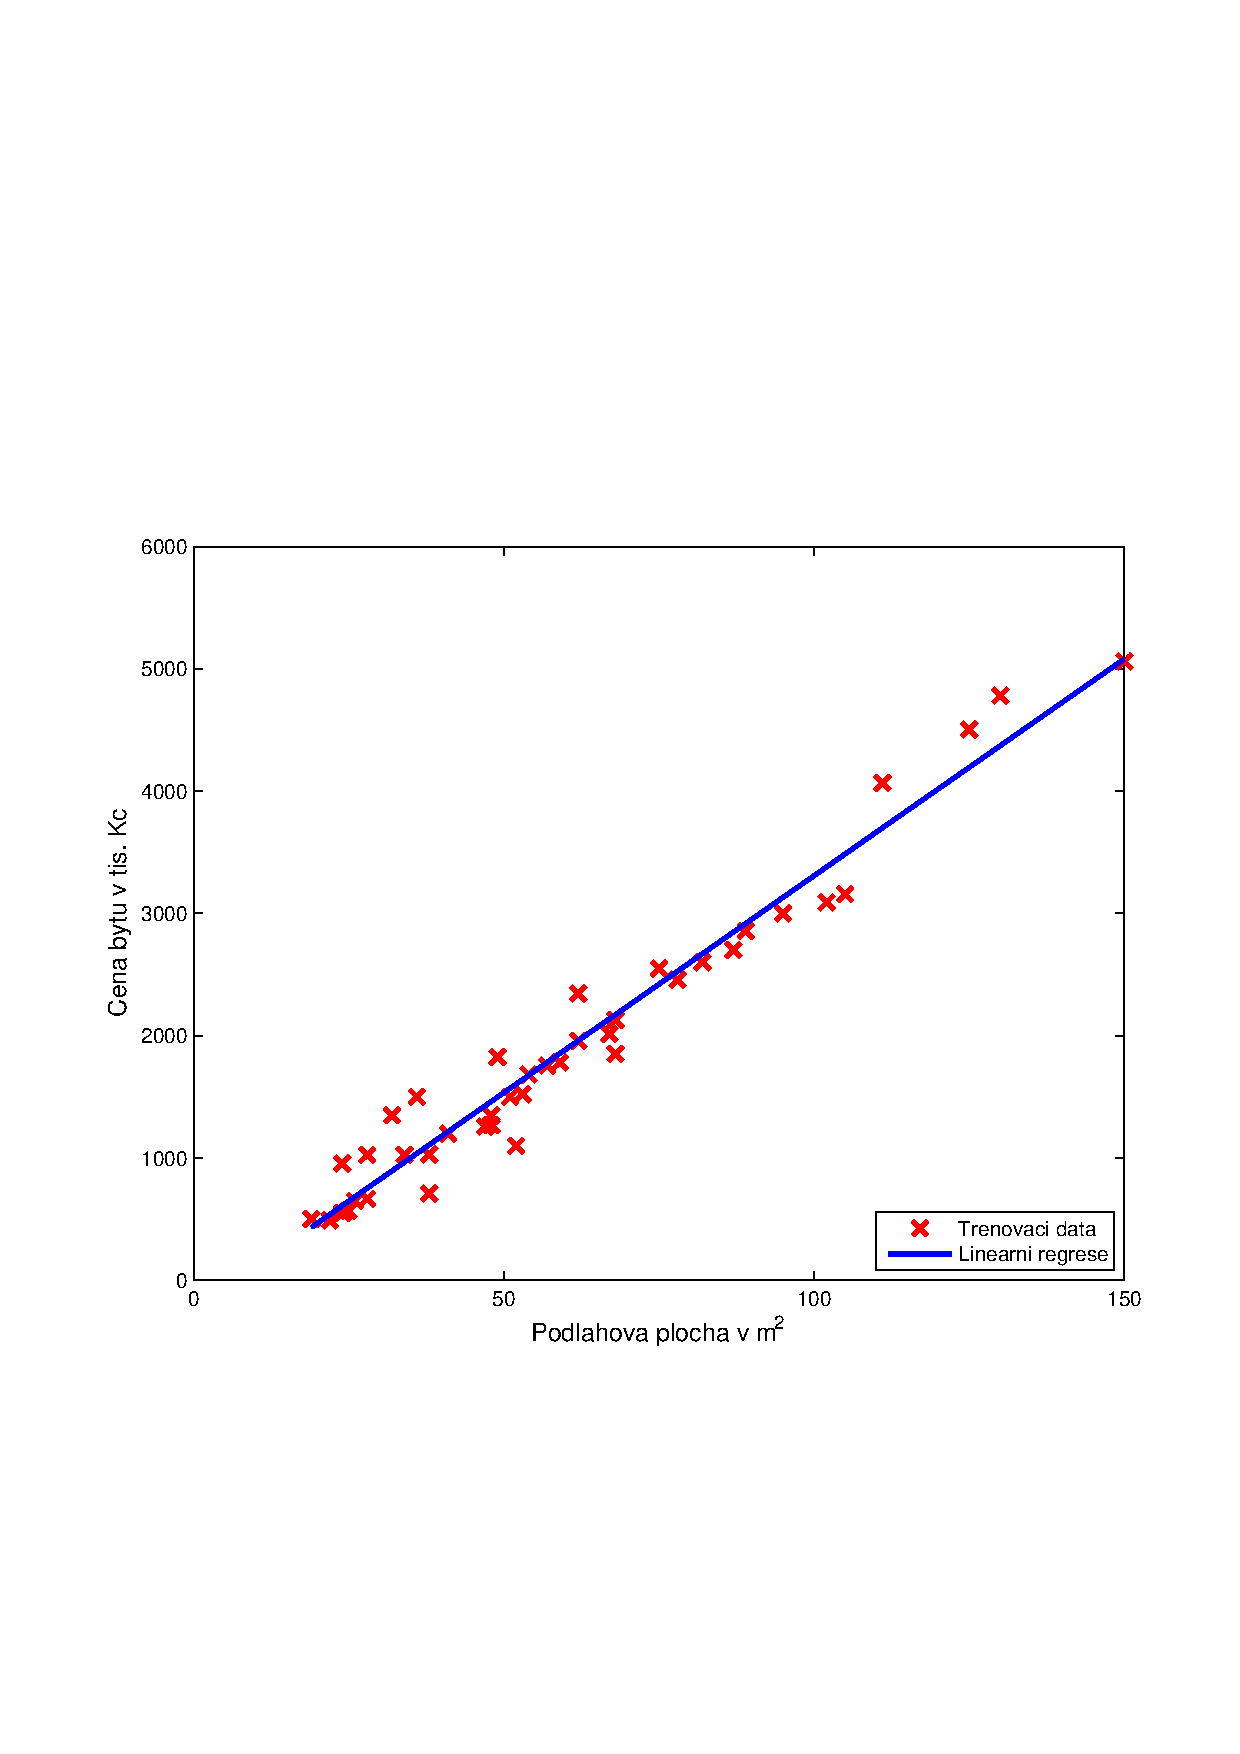
\includegraphics[scale = 0.5, trim = 2.5cm 7cm 2cm 9cm]{./Img/LinearniRegrese/cena_plocha_linear_regrese.pdf}
	\caption{Výsledná lineární regrese našeho úvodního příkladu po výpočtu gradientním algoritmem.}
	\label{fig:cena_plocha_linear_regrese}
\end{figure}


\newpage









%----------------VICEROZMERNA-LINEARNI-REGRESE-------------------
\subsection{Vícerozměrná lineární regrese}
\label{sec:LinearniRegreseVicePromennych}

\par{V sekci \ref{sec:LinearniRegreseUceniSUcitelem} byla představena lineární regrese o~jedné proměnné na příkladě predikce ceny bytu (výstup $y$) v závislosti na velikosti podlahové plochy $m^2$ (vstup $x$).}

\par{V případě vícerozměrné lineární regrese si můžeme představit, že nemáme pouze velikost podlahové plochy bytu, ale výsledná cena závisí i dalších parametrech bytu, viz tabulka \ref{tab:vzorkyND}.

\begin{table}[!ht]
\centering
\begin{tabular}{c|c|c|c|c}
	{Velikost bytu} & {Počet místností} & {Počet poschodí} & {Stáří bytu} & {Cena bytu}\\
	{$x_1$} & {$x_2$} & {$x_3$} & {$x_4$} & {$y$}\\
	\hline
	{19} & {5} & {1} & {45} & {500}\\
	{22} & {3} & {2} & {40} & {490}\\
	{25} & {2} & {1} & {30} & {568}\\
	{$\ldots$} & {$\ldots$} & {$\ldots$} & {$\ldots$} & {$\ldots$}
\end{tabular}
\caption{Příklady vícerozměrných trénovacích vzorků.}
\label{tab:vzorkyND}
\end{table}}

\par{Proměnnou $n$ budeme označovat počet příznaků (v~našem případě v tabulce \ref{tab:vzorkyND} $x_{1, \ldots , 4}$, proto $n = 4$.) Dále budeme stále jako u jednorozměrného případu označovat vstupní příznaky (všechny = sloupcový vektor) $\bm{x}^{\left( i \right)}$ pro $i$-tý trénovací vzor. A~hodnota jednotlivého $j$-tého příznaku $i$-tého trénovacího vzoru bude označována $\bm{x}^{\left( i \right)}_{j}$.}

\par{V~případě jednorozměrné lineární regrese byla naše hypotéza $h_\Theta$ reprezentována
\begin{equation}
	h_{\bm{\Theta}} \left( x \right) = \vartheta_0 + \vartheta_1 x,
	\label{eq:1Dhypothesis}
\end{equation}
v~našem vícerozměrném případě nabývá tvaru
\begin{equation}
	h_{\bm{\Theta}} \left( \bm{x} \right) = \vartheta_0 + \vartheta_1 x_1 + \vartheta_2 x_2 + \vartheta_3 x_3 + \vartheta_4 x_4 .
	\label{eq:NDhypothesis}
\end{equation}
V~případě \ref{eq:1Dhypothesis} i \ref{eq:NDhypothesis} je možné si všimnout, že $x_0 = 1$ čehož dále využijeme, přesněji $\bm{x}^{\left( i \right)}_0 = 1$ z důvodu dodržení konvence. Proto $\bm{x} \in \mathrm{R}^{n + 1}$ a to samé platí pro parametry $\bm{\Theta} \in \mathrm{R}^{n + 1}$.}

\subsubsection*{Poznámka}
\par{V~našem příkladě odpovídají
\begin{equation}
	\bm{x} = \left[ x_0,~x_1,~x_2,~x_3,~x_4 \right]^{\top}
\end{equation}
a
\begin{equation}
	\bm{\Theta} = \left[ \vartheta_0,~\vartheta_1,~\vartheta_2,~\vartheta_3,~\vartheta_4 \right]^{\top}.
\end{equation}}

\par{Obecněji lze vícerozměrnou hypotézu zapsat jako
\begin{equation}
	h_{\bm{\Theta}} \left( \bm{x} \right) = \vartheta_0 + \vartheta_1 x_1 + \vartheta_2 x_2 + \ldots + \vartheta_n x_n,
	\label{eq:NDhypothesisObecne}
\end{equation}
neboli jednoduše jako součin vektorů (vnitřní produkt)
\begin{equation}
	h_{\bm{\Theta}} \left( \bm{x} \right) = \bm{\Theta}^{\top} \bm{x}.
	\label{eq:NDhypothesisObecneVektorove}
\end{equation}}


\newpage












%----------------GRADIENT-DESCENT-VICEROZMERNY--------------------
\subsection{Gradientní algoritmus - vícerozměrná verze}
\label{sec:LinearniRegreseGradientDescentVicerozmerny}

\par{Budeme potřebovat hypotézu
\begin{equation}
	h_{\bm{\Theta}} \left( \bm{x} \right) = \bm{\Theta}^{\top} \bm{x} = \vartheta_0 x_0 + \vartheta_1 x_1 + \vartheta_2 x_2 + \ldots + \vartheta_n x_n,
\end{equation}
kde $x_0 = 1$, dále parametry $\bm{\Theta} = \left[ \vartheta_0,~\vartheta_1,~\vartheta_2,~\ldots,~\vartheta_4 \right]^{\top}$ a vícerozměrnou ztrátovou funkci
\begin{equation}
	J \left( \bm{\Theta} \right) = \frac{1}{2m} \sum_{i = 1}^{m} \left( h_{\bm{\Theta}} \left( \bm{x}^{\left( i \right)} \right) - y^{\left( i \right)} \right)^2.
\end{equation}}

\par{Gradientní algoritmus pak bude mít tvar: opakuj
\begin{equation}
	\vartheta_j = \vartheta_j - \alpha \frac{\partial}{\partial \vartheta_j} J \left( \bm{\Theta} \right),
	\label{eq:algoritmusNDgradientDescent}
\end{equation}
současně aktualizovat parametry pro všechny $j = 0, \ldots, n$.}

\par{Vztah z rovnice \ref{eq:algoritmusNDgradientDescent} lze zapsat jako
\begin{equation}
	\frac{\partial}{\partial \vartheta_j} J \left( \bm{\Theta} \right) = \frac{1}{m} \sum_{i = 1}^{m} \left( h_{\bm{\Theta}} \left( \bm{x}^{\left( i \right)} \right) - y^{\left( i \right)} \right) \bm{x}^{\left( i \right)}_j
	\label{eq:derivaceNDgradientDescent}	
\end{equation}
a po spojení rovnic 	\ref{eq:algoritmusNDgradientDescent} a \ref{eq:derivaceNDgradientDescent} získáváme výsledný tvar
\begin{equation}
	\vartheta_j = \vartheta_j - \alpha \frac{1}{m} \sum_{i = 1}^{m} \left( h_{\bm{\Theta}} \left( \bm{x}^{\left( i \right)} \right) - y^{\left( i \right)} \right) \bm{x}^{\left( i \right)}_j,
	\label{eq:NDgradientDescentVysledna}
\end{equation}
pokud bychom výslednou rovnici \ref{eq:NDgradientDescentVysledna} rozepsali pro první dva parametry $\vartheta_0$ a $\vartheta_1$ dostali bychom
\begin{eqnarray}
	&\vartheta_0 &= \vartheta_0 - \alpha \frac{1}{m} \sum_{i = 1}^{m} \left( h_{\bm{\Theta}} \left( \bm{x}^{\left( i \right)} \right) - y^{\left( i \right)} \right) \bm{x}^{\left( i \right)}_0, \quad \bm{x}^{\left( i \right)}_0 = 1\\
	&\vartheta_1 &= \vartheta_1 - \alpha \frac{1}{m} \sum_{i = 1}^{m} \left( h_{\bm{\Theta}} \left( \bm{x}^{\left( i \right)} \right) - y^{\left( i \right)} \right) \bm{x}^{\left( i \right)}_1\\
	\nonumber
	&\vdots
\end{eqnarray}}




\newpage









%----------------FEATURES-SCALING-------------------
\subsection{Features scaling}
\label{sec:featuresScaling}

\par{V~této podkapitole si řekneme něco o~velikosti příznaků. První a~nejdůležitější věcí je normování velikostí příznaků na stejnou velikost. Neboli, pokud použijeme opět náš příklad nákupu bytu a~definujeme si velikost bytu v~$dm^2$ (příznak $x_1$) a~počet místností bytu (příznak $x_2$) a~řekněme že:
\begin{eqnarray}
	\nonumber
	&x_1 &\in \langle 5000, 20000 \rangle,\\
	\nonumber
	&x_2 &\in \langle 1, 5 \rangle,
\end{eqnarray}
tak bude pro gradientní metodu velmi obtížné a~více výpočetně náročné (bude nutno spočítat více iterací) nalézt minimum. Proto je důležité, aby všechny příznaky měli stejné škálování. V~našem případě by to znamenalo 

\begin{eqnarray}
	\nonumber
	&x_1 &= \frac{\mbox{velikost bytu}}{20000},\\
	\nonumber
	&x_2 &= \frac{\mbox{počet místností}}{5}.
\end{eqnarray}
Více obecně lze říci, že se většinou volí normování na interval $\langle -1, 1 \rangle$.}

\subsubsection*{Mean normalization}
\par{Velice častá normalizace střední hodnotou $\mu$, konkrétně pro $i$-tý příznak
\begin{equation}
	x_i \leftarrow \frac{x_i - \mu_i}{max - min}
\end{equation}
nebo
\begin{equation}
	x_i \leftarrow \frac{x_i - \mu_i}{std}
\end{equation}
($std$ = Standard deviation).

















%----------------NORMAL-EQUATION------------------
\subsection{Analytické řešení}
\label{sec:normalEquation}

\par{V této sekci si ukážeme jak lze vypočítat minimum naší ztrátové funkce $J \left( \bm{\Theta} \right)$ analyticky.}

\subsubsection*{Příklad:}
\par{Předpokládejme 1D příklad ($\vartheta \in \mathcal{R}$), kdy máme ztrátovou funkci $J \left( \vartheta \right)$, která je funkcí jedné reálné proměnné
\begin{equation}
	J \left( \vartheta \right) = a \vartheta^2 + b \vartheta + c
\end{equation}}

\par{Pro minimalizaci naší kvadratické ztrátové funkce využijeme hledání extrému (položíme derivaci rovnou nule)
\begin{equation}
	\frac{\mathrm{d}}{\mathrm{d}\vartheta} J \left( \vartheta \right) = \ldots \equiv 0
\end{equation}
a vyřešíme pro parametr $\vartheta$.}

\par{Více obecněji pro $\bm{\Theta} \in \mathcal{R}^{n+1}$ bude naše ztrátová funkce nabývat tvaru
\begin{equation}
	J \left( \vartheta_0,~\vartheta_1,~\ldots,~\vartheta_m \right) = \frac{1}{2m} \sum_{i=1}^{m} \left( h_{\bm{\Theta}} \left( \bm{x}^{\left( i \right)} \right) - y^{\left( i \right)} \right)^2
\end{equation}
dále položíme parciální derivace podle jednotlivých parametrů rovny nule (pro všechny $j$)
\begin{equation}
	\frac{\partial}{\partial \vartheta_j} = \ldots \equiv 0
\end{equation}
a vyřešíme pro parametry $\vartheta_0,~\vartheta_1,~\ldots,~\vartheta_m$.}

\par{Pro složení obyčejné rovnice budeme potřebovat matici $\bm{X} \in \mathcal{R}^{m \times \left( n + 1 \right)}$, která v řádcích obsahuje jednotlivé vektory $\left( \bm{x}^{\left( i \right)} \right)^{\top}$ a výstupní sloupcový vektor $\bm{y} \in \mathcal{R}^{m}$. Kde $m$ je počet trénovacích vzorků (velikost trénovací množiny) a $n$ je počet příznaků, kde $\bm{x}_0^{\left( i \right)} = 0$.}

\par{Nyní můžeme zapsat předpis pro výpočet parametrů $\bm{\Theta}$ analyticky
\begin{equation}
	\bm{\Theta} = \left( \bm{X}^{\top} \bm{X} \right)^{-1} \bm{X}^{\top} \bm{y}.
\end{equation}
Pro analytické řešení není nutné příznaky normovat, jako v případě gradientního algoritmu, na stejné měřítko, jak je popsáno v sekci \ref{sec:featuresScaling}.}





















%----------------NORMAL-EQUATION------------------
\subsection{Gradientní algoritmus vs. analytické řešení}
\label{sec:GAvsAR}

\par{V této sekci budou zmíněny výhody a nevýhody gradientního algoritmu versus analytického řešení. Velikost trénovací množiny $m$ a počet příznaků $n$.
\begin{center}
\begin{tabular}{c|c}
	{Gradientní algoritmus} & {Analytické řešení} \\
	\hline
	{Nutno zvolit konstantu učení $\alpha$.} & {Není nutné volit konstantu učení $\alpha$.}\\
	{Potřebuje mnoho iterací.} & {Nepotřebuje iterovat.}\\
	{Pracuje dobře, když je $n$ velké.} & {Pomalé pokud je $n$ velké.}\\
	{~} & {Nutnost vypočítat inverzi $\left( \bm{X}^{\top} \bm{X} \right)^{-1}$.}\\
	{~} & {(Složitost $\mathcal{O}\left( n^3 \right)$).}\\
	{Zvolit pokud $n > 10^6$.} & {Zvolit pokud $n < 10^4$.}
\end{tabular}
\end{center}}


\newpage
















\section{Binární regrese - klasifikace}
\label{sec:BinarniRegrese}

\par{Logistická regrese je označení metody matematické statistiky zabývající se problematikou odhadu pravděpodobnosti nějakého jevu (závisle proměnné) na základě určitých známých skutečností (nezávisle proměnných), které mohou ovlivnit výskyt jevu. Událost, zda zkoumaný jev nastal, se modeluje pomocí náhodné veličiny, která nabývá hodnoty 0, pokud jev nenastal, nebo 1, pokud jev nastal.}











%------------KLASIFIKACE---------------------------------------------------------
\subsection{Klasifikace}
\label{sec:BinarniRegreseKlasifikace}

\par{Na úvod si uveďme několik klasifikačních příkladů:
\begin{center}
	\textbf{Spam:} je spam / není spam ?\\
	\textbf{Online transakce:} podvodné ano / ne ?\\
	\textbf{Nádor:} zhoubný / nezhoubný?
\end{center}
Z příkladů je zřejmé, že se jedná o rozhodnutí mezi dvěma možnostmi, tedy $y \in \{ 0, 1 \}$, kde $0$ je \uv{negativní třída} (nezhoubný nádor) a~$1$ je pozitivní třída (zhoubný nádor). Pokud máme $y \in \{ 0, 1 \}$ jedná se o~klasifikaci do dvou tříd, dále existuje klasifikace do více tříd, kde $y \in \{ 0, 1, 2, 3, \ldots \}$. V následujících kapitolách se budeme zabývat klasifikací do dvou tříd.}
\par{Nyní se dostáváme k problému jak vyvinout klasifikační algoritmus, což si můžeme ukázat na příkladu trénovací sady pro úlohu klasifikace nádorů. Nádor může být buď zhoubný nebo nezhoubný, tedy buďto 1 nebo 0. Dostupná data pro náš příklad jsou na obrázku \ref{fig:nadory1}.
\begin{figure}[!ht]
	\centering
	%trim option's parameter order: left bottom right top
	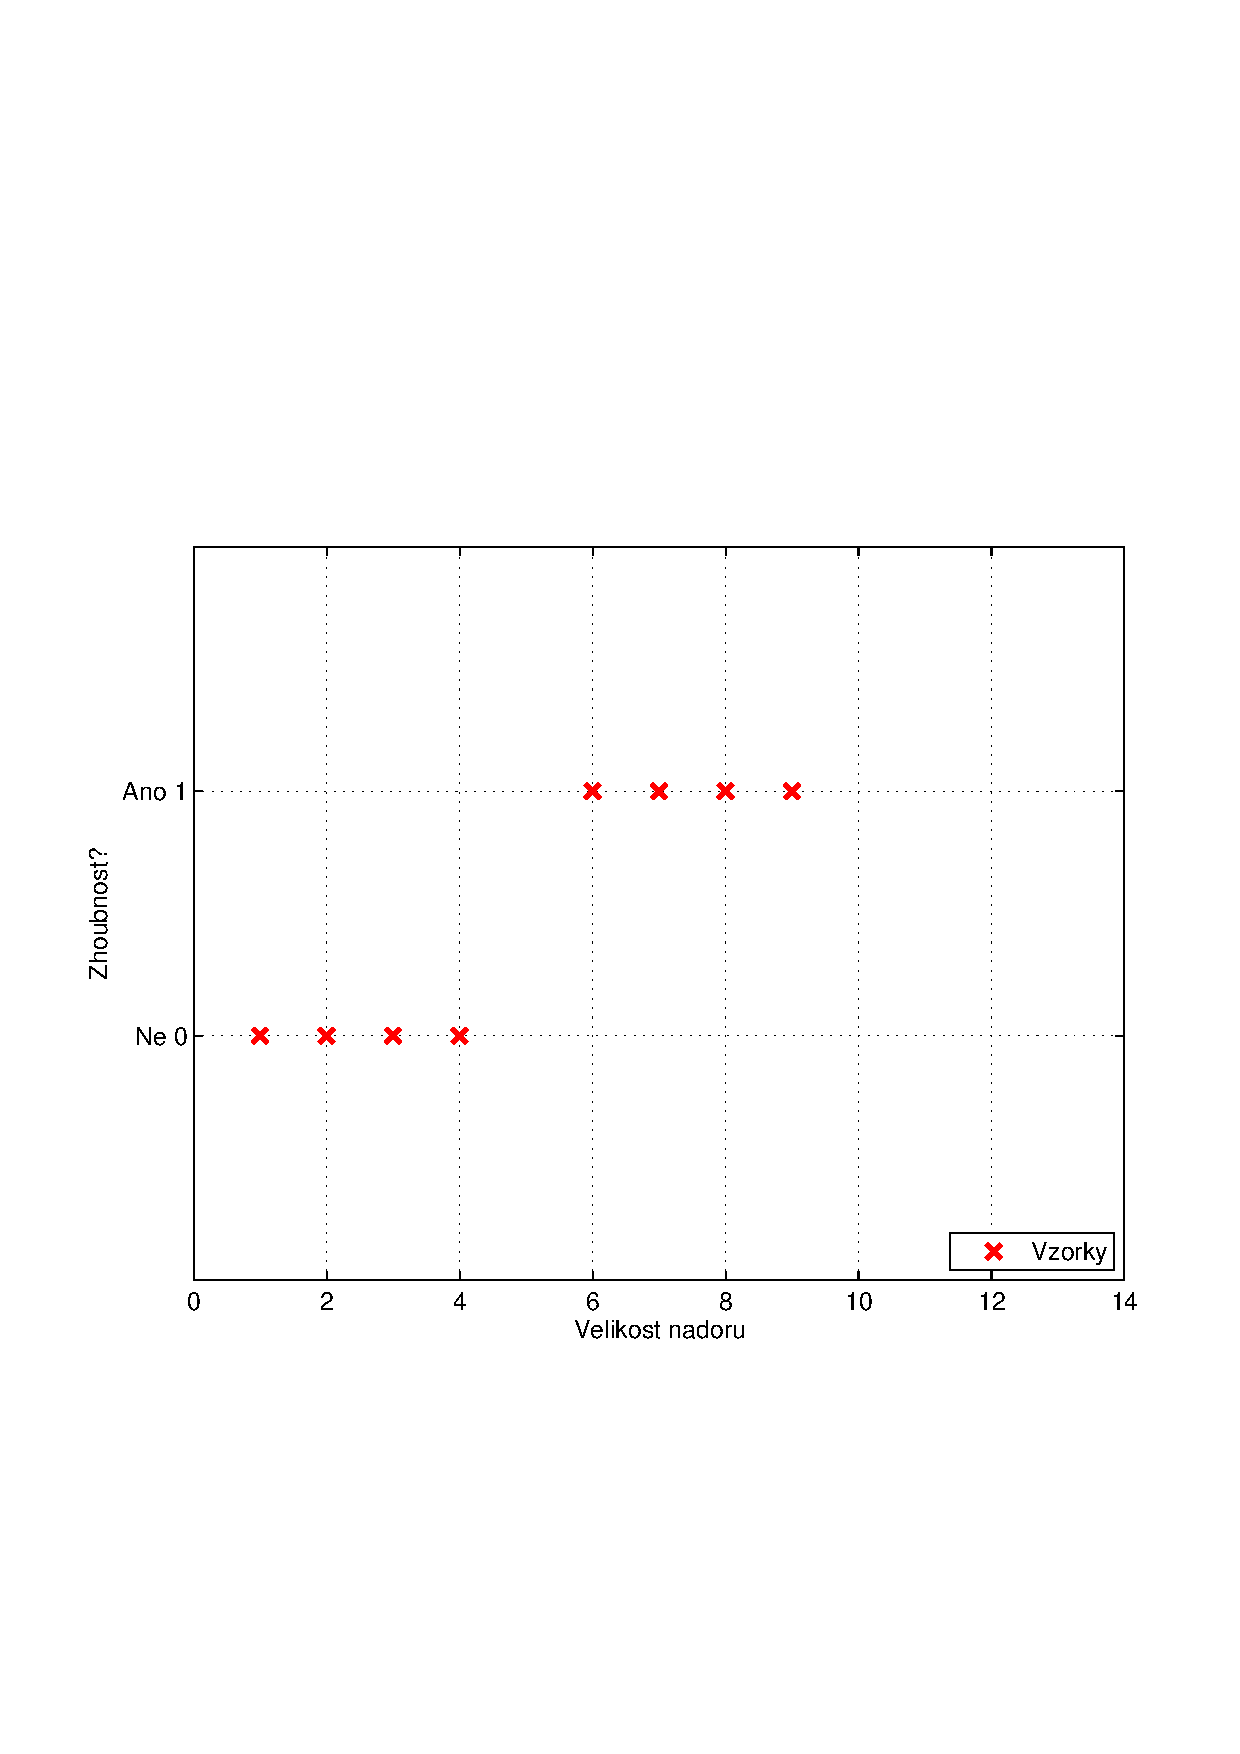
\includegraphics[width = 0.48\textwidth, trim = 2.5cm 7cm 2cm 9cm]{./Img/BinarniRegrese/prikladNadory/tumor_1st_example.pdf}
	\caption{Trénovací data.}
	\label{fig:nadory1}
\end{figure}}
\pagebreak

\par{Jedna z~věcí, kterou bychom mohli udělat, je aplikace algoritmu lineární regrese, který známe z~kapitoly \ref{sec:LinearniRegrese}. Výsledek aplikace hypotézy
\begin{equation}
	h_{\bm{\Theta}} \left( \bm{x} \right) = \bm{\Theta}^{\top} \bm{x}
\end{equation}
lze vidět na Obr. \ref{fig:nadory2}.}

\par{Pokud bychom chtěli udělat predikci ze získané hypotézy, tak můžeme využít klasifikátoru na základě prahování. Tedy hodnotu po jejíž překročení vzorek spadá již do druhé třídy, v~případě binární regrese je to hodnota 0.5. Chceme tedy určit
\begin{eqnarray}
	\label{eq:prah1}
	h_{\bm{\Theta}} \left( \bm{x} \right) \geq 0.5, \quad \mathrm{predikuj~} y = 1,\\
	\label{eq:prah2}
	h_{\bm{\Theta}} \left( \bm{x} \right) < 0.5, \quad \mathrm{predikuj~} y = 0.
\end{eqnarray}
Tento poznatek je reprezentován na Obr. \ref{fig:nadory3}.

\begin{figure}[!ht]
	\centering
	\begin{minipage}[t]{0.48\textwidth}
		%trim option's parameter order: left bottom right top
		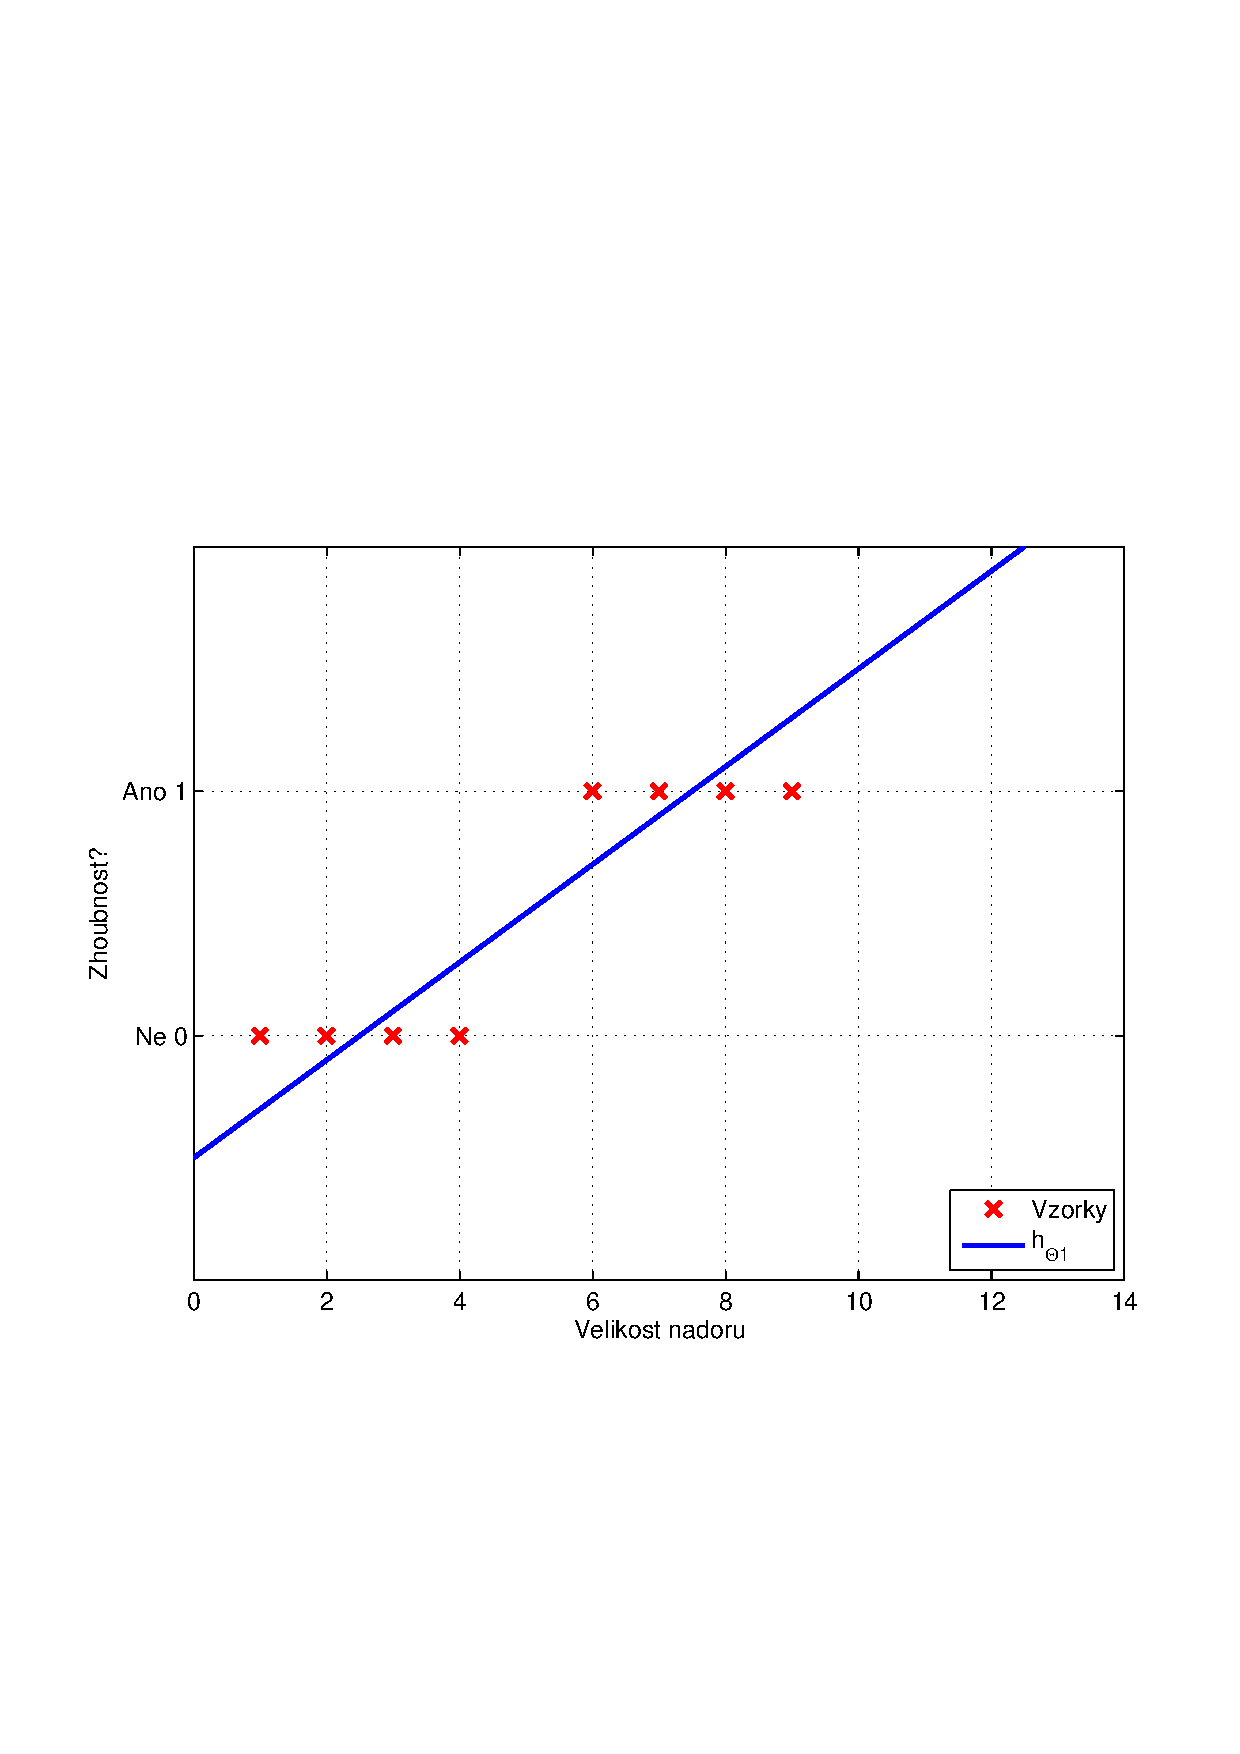
\includegraphics[width = \textwidth, trim = 2.5cm 7cm 2cm 9cm]{./Img/BinarniRegrese/prikladNadory/tumor_2st_example.pdf}
		\caption{Lineární regrese.}
		\label{fig:nadory2}
	\end{minipage}%
	\hfill
	\begin{minipage}[t]{0.48\textwidth}
		%trim option's parameter order: left bottom right top
		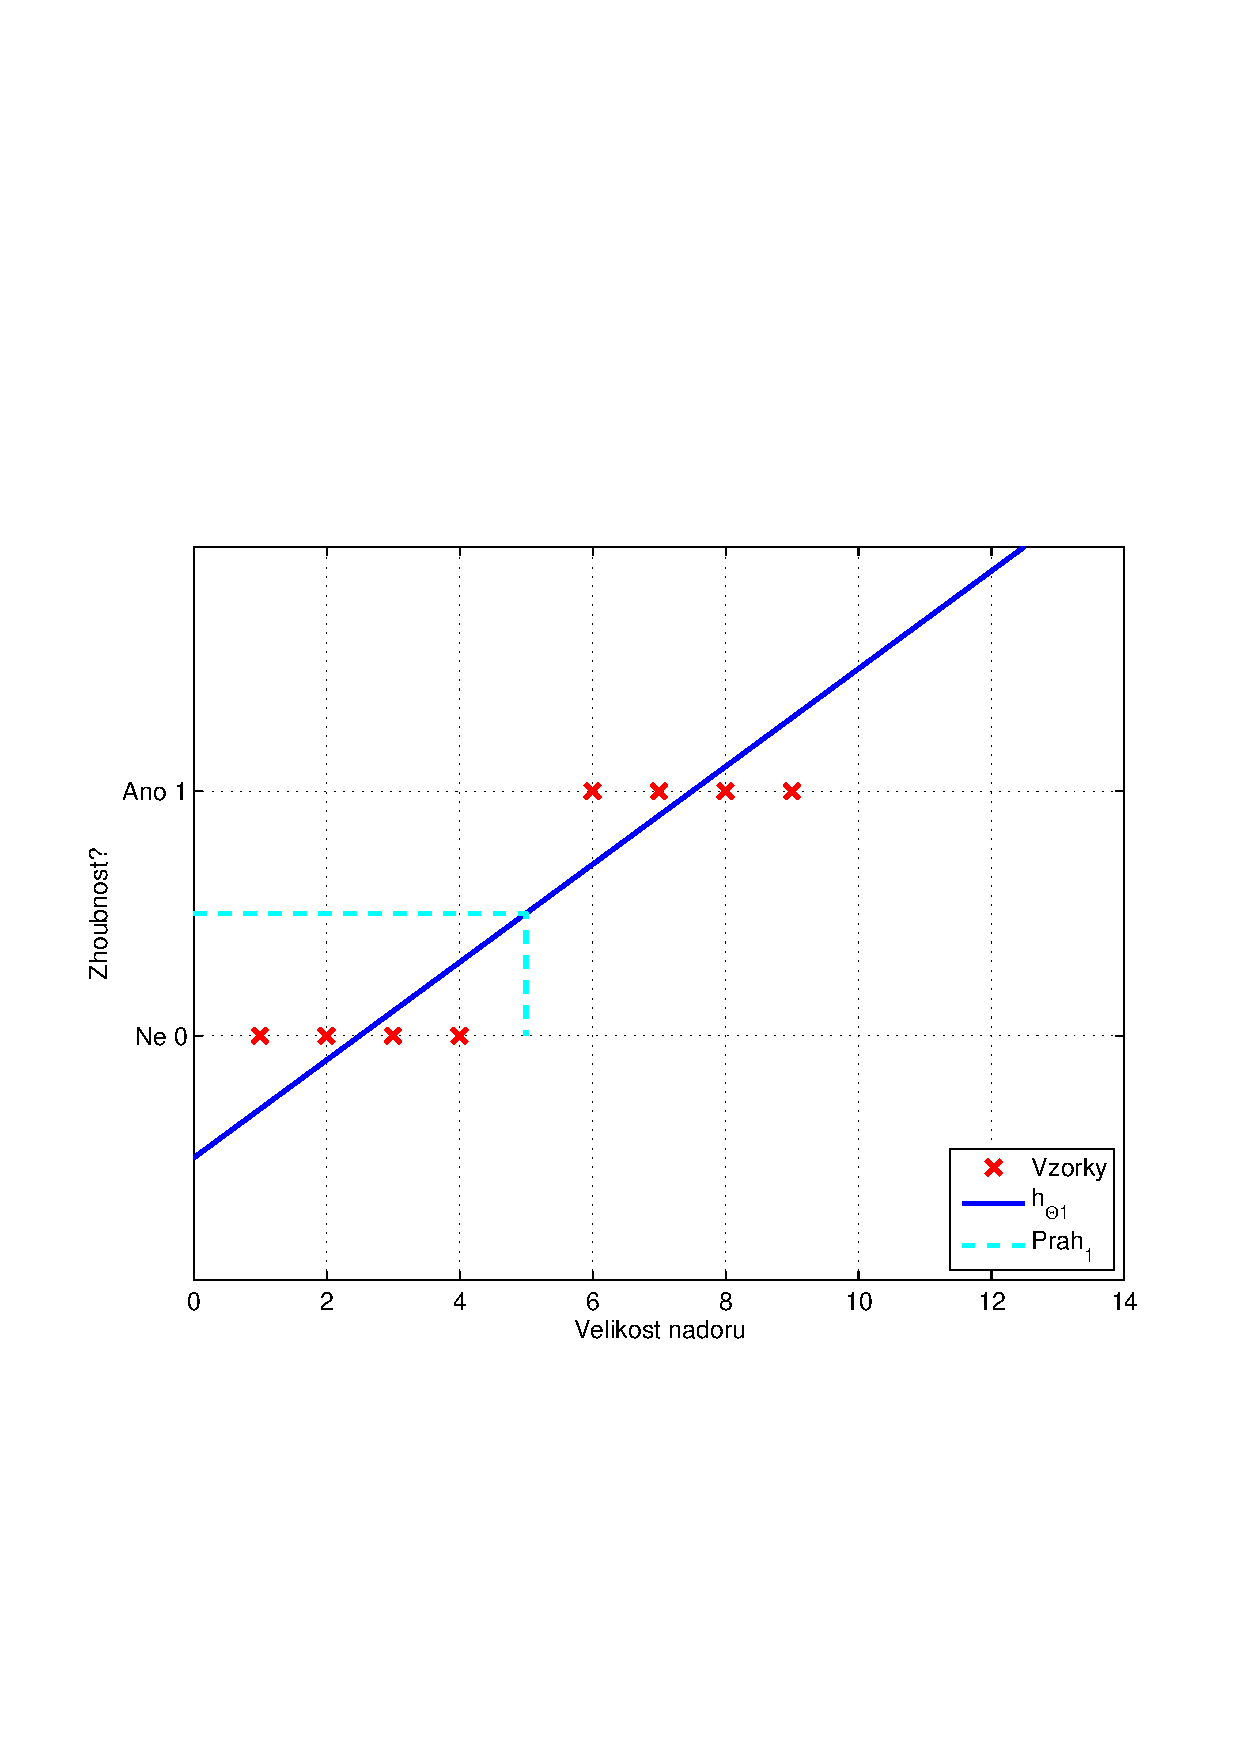
\includegraphics[width = \textwidth, trim = 2.5cm 7cm 2cm 9cm]{./Img/BinarniRegrese/prikladNadory/tumor_3st_example.pdf}
		\caption{Lineární regrese - určení rozhodovacího prahu.}
		\label{fig:nadory3}
	\end{minipage}%
\end{figure}}

\par{V tomto příkladě jsme si ukázali, že lineární regrese dělá něco co by se dalo považovat za řešení klasifikačního problému. Na následujícím rozšíření našeho příkladu bude ukázáno, že tomu tak není.}

\par{Rozšíříme náš příklad o~další vzorky viz Obr. \ref{fig:nadory4}, kde nám přibyly dva vzorky více vpravo. Po aplikování lineární regrese, na rozšířená data, získáváme výsledek, který lze vidět na Obr. \ref{fig:nadory5}. Aktuální hypotéza $h_{\bm{\Theta} 2}$ již nesplňuje podmínky definované vztahy \ref{eq:prah1} a~\ref{eq:prah2}, jelikož první vzorek, který má být vyhodnocen jako zhoubný by v tomto případě byl vyhodnocen jako nezhoubný, což může zásadně ovlivnit něčí život.

\begin{figure}[!ht]
	\centering
	\begin{minipage}[t]{0.48\textwidth}
		%trim option's parameter order: left bottom right top
		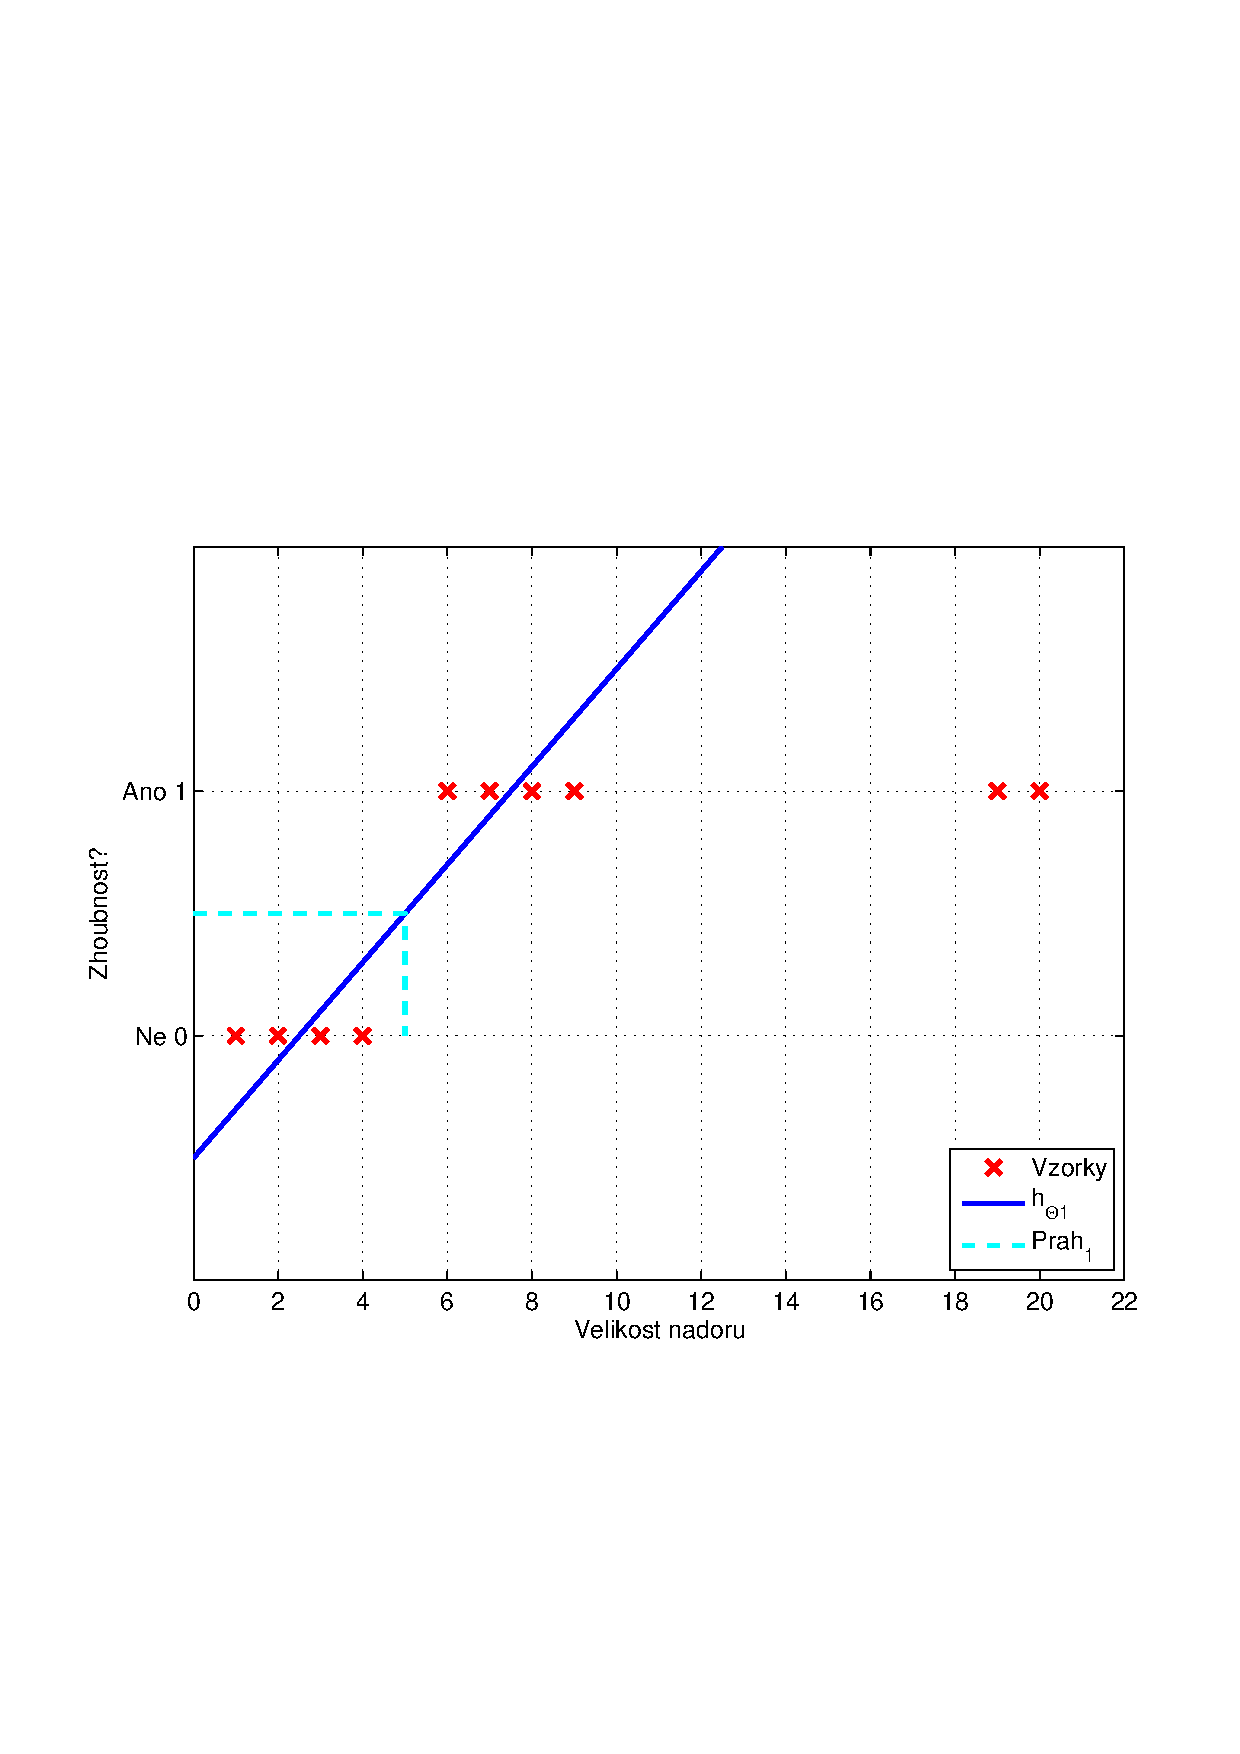
\includegraphics[width = \textwidth, trim = 2.5cm 7cm 2cm 9cm]{./Img/BinarniRegrese/prikladNadory/tumor_4st_example.pdf}
		\caption{Rozšíření trénovací množiny dat o dva vzorky vpravo.}
		\label{fig:nadory4}
	\end{minipage}%
	\hfill
	\begin{minipage}[t]{0.48\textwidth}
		%trim option's parameter order: left bottom right top
		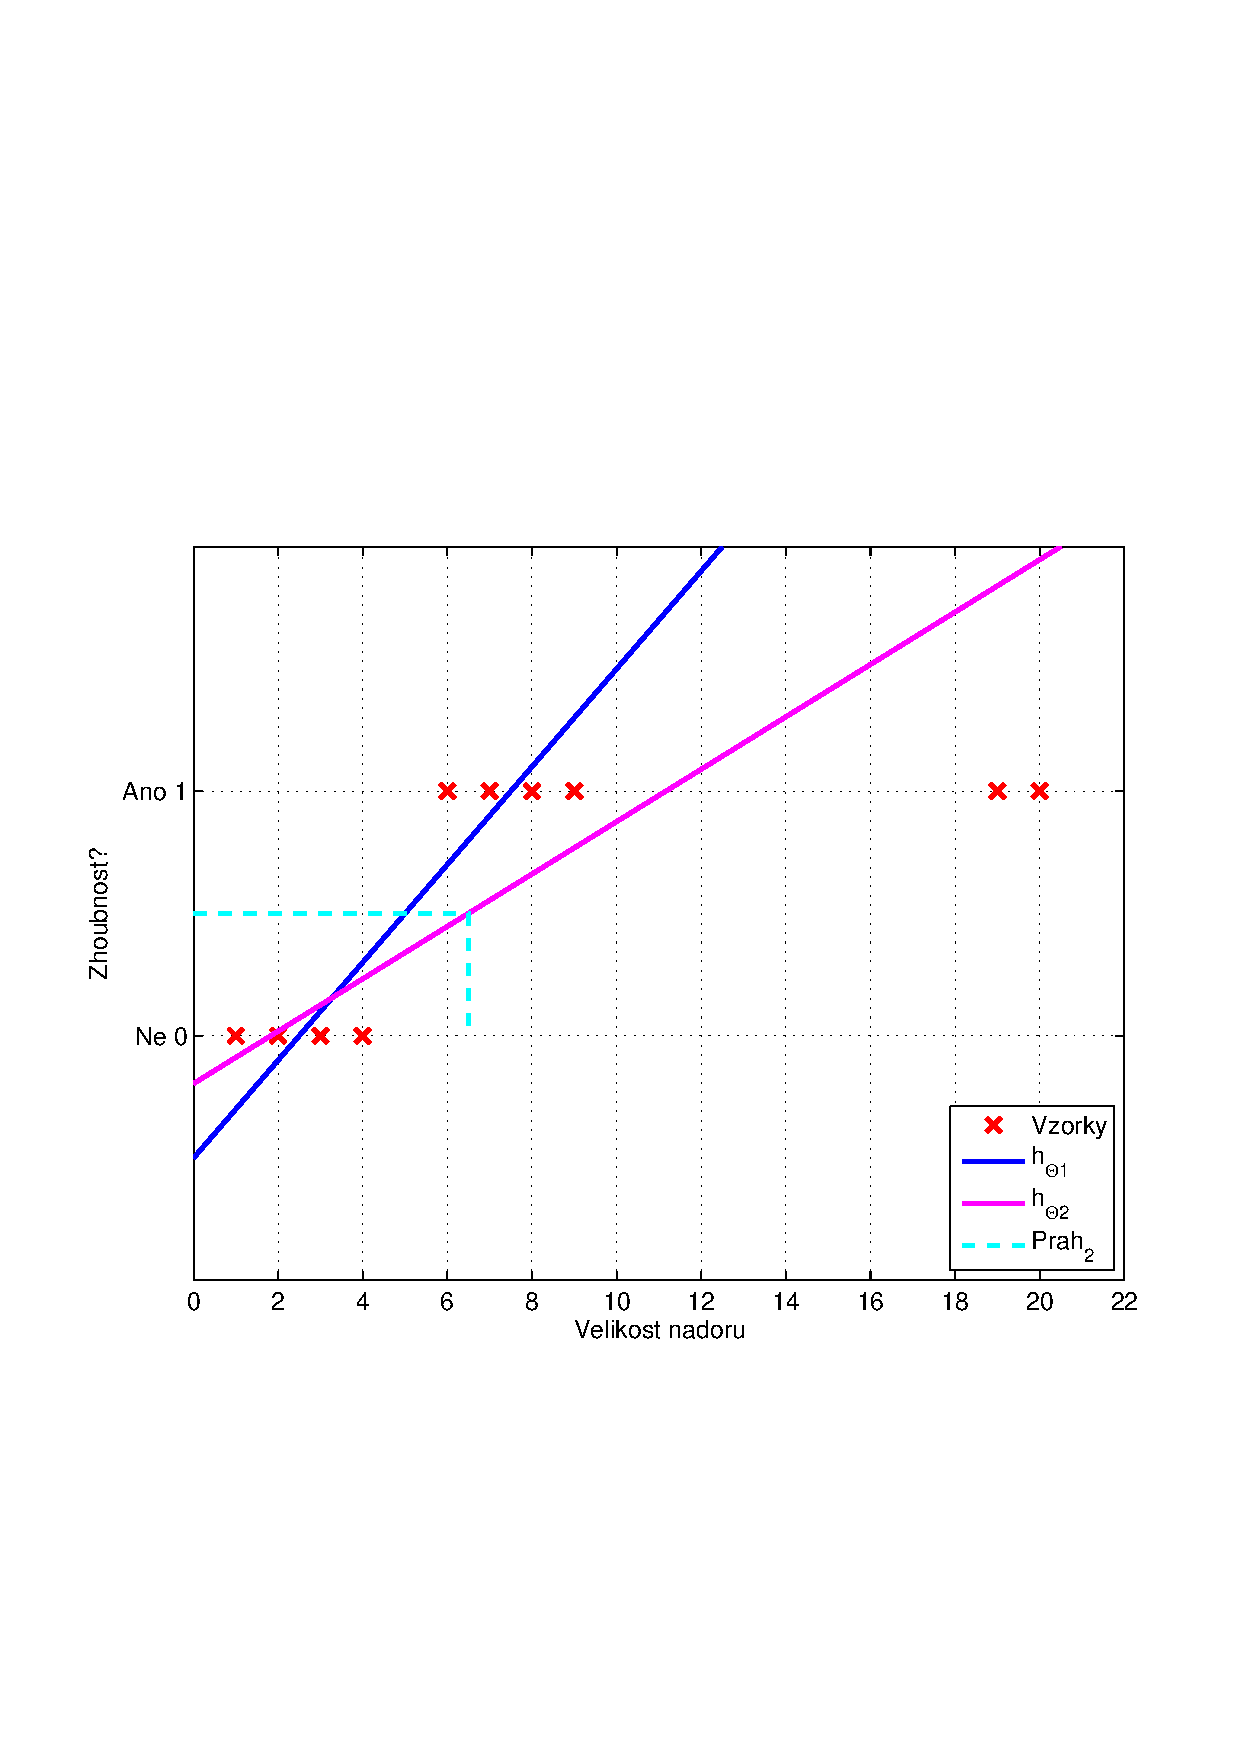
\includegraphics[width = \textwidth, trim = 2.5cm 7cm 2cm 9cm]{./Img/BinarniRegrese/prikladNadory/tumor_5st_example.pdf}
		\caption{Lineární regrese - určení rozhodovacího prahu a zobrazení jeho selhání při predikci.}
		\label{fig:nadory5}
	\end{minipage}%
\end{figure}}

\par{V tomto příkladě, lépe řečeno protipříkladě jsme si ukázali, proč je nevhodné využívat lineární regresi jako klasifikační algoritmus. Ve většině případů nefunguje správně. Pro klasifikaci na základě lineární regrese můžeme získat výsledek hypotézy $h_{\bm{\Theta}} > 1$ nebo $h_{\bm{\Theta}} < 0$, přičemž výsledek binární klasifikace je pouze $y = 0$ nebo $y = 0$. Proto bude nutné v~dalších kapitolách přijít se sofistikovanějším postupem binární regrese (klasifikace), která splňuje podmínku $0 \leq h_{\bm{\Theta}} \leq 1$.}




\newpage













%-----REPREZENTACE-HYPOTEZY-------------------------------------------------------------
\subsection{Reprezentace hypotézy}
\label{sec:BinarniRegreseReprezentaceHypotezy}

\par{V této kapitole si ukážeme, jak správně reprezentovat hypotézu, tedy jakou funkci je vhodné použít v případě problému klasifikace.}

\par{V sekci \ref{sec:BinarniRegreseKlasifikace} jsme zjistili, že bychom si pro binární regresní model přáli, aby platilo
\begin{equation}
	0 \leq h_{\bm{\Theta}} \left( \bm{x} \right) \leq 1,
\end{equation}
tedy aby výstupní hodnota byla mezi 0 a 1 (včetně). Pro reprezentaci hypotézy lineární regrese platí
\begin{equation}
	h_{\bm{\Theta}} \left( \bm{x} \right) = \bm{\Theta}^{\top} \bm{x},
\end{equation}
tuto hypotézu upravíme na tvar
\begin{equation}
	h_{\bm{\Theta}} \left( \bm{x} \right) = g \left( \bm{\Theta}^{\top} \bm{x} \right),
	\label{eq:Ghypoteza}
\end{equation}
kde funkce $g$ je definována následovně
\begin{equation}
	g \left( \bm{z} \right) = \frac{1}{1 + e^{-\bm{z}}},
	\label{eq:funkceSigmoidy}
\end{equation}
tato funkce se nazývá sigmoid funkce (Sigmoid function) nebo logistická/binární funkce (Logistic function). Jméno logistická funkce je důvod, proč vznik termín logistická/binární regrese. Pokud spojíme rovnice \ref{eq:Ghypoteza} a \ref{eq:funkceSigmoidy} získáme tvar
\begin{equation}
	h_{\bm{\Theta}} \left( \bm{x} \right) =  \frac{1}{1 + e^{- \bm{\Theta}^{\top} \bm{x}}} 
\end{equation}
a průběh grafu funkce $g \left( \bm{z} \right)$ lze vidět na Obr. \ref{fig:sigmoidFunction}.
\begin{figure}[!ht]
	\centering
	%trim option's parameter order: left bottom right top
	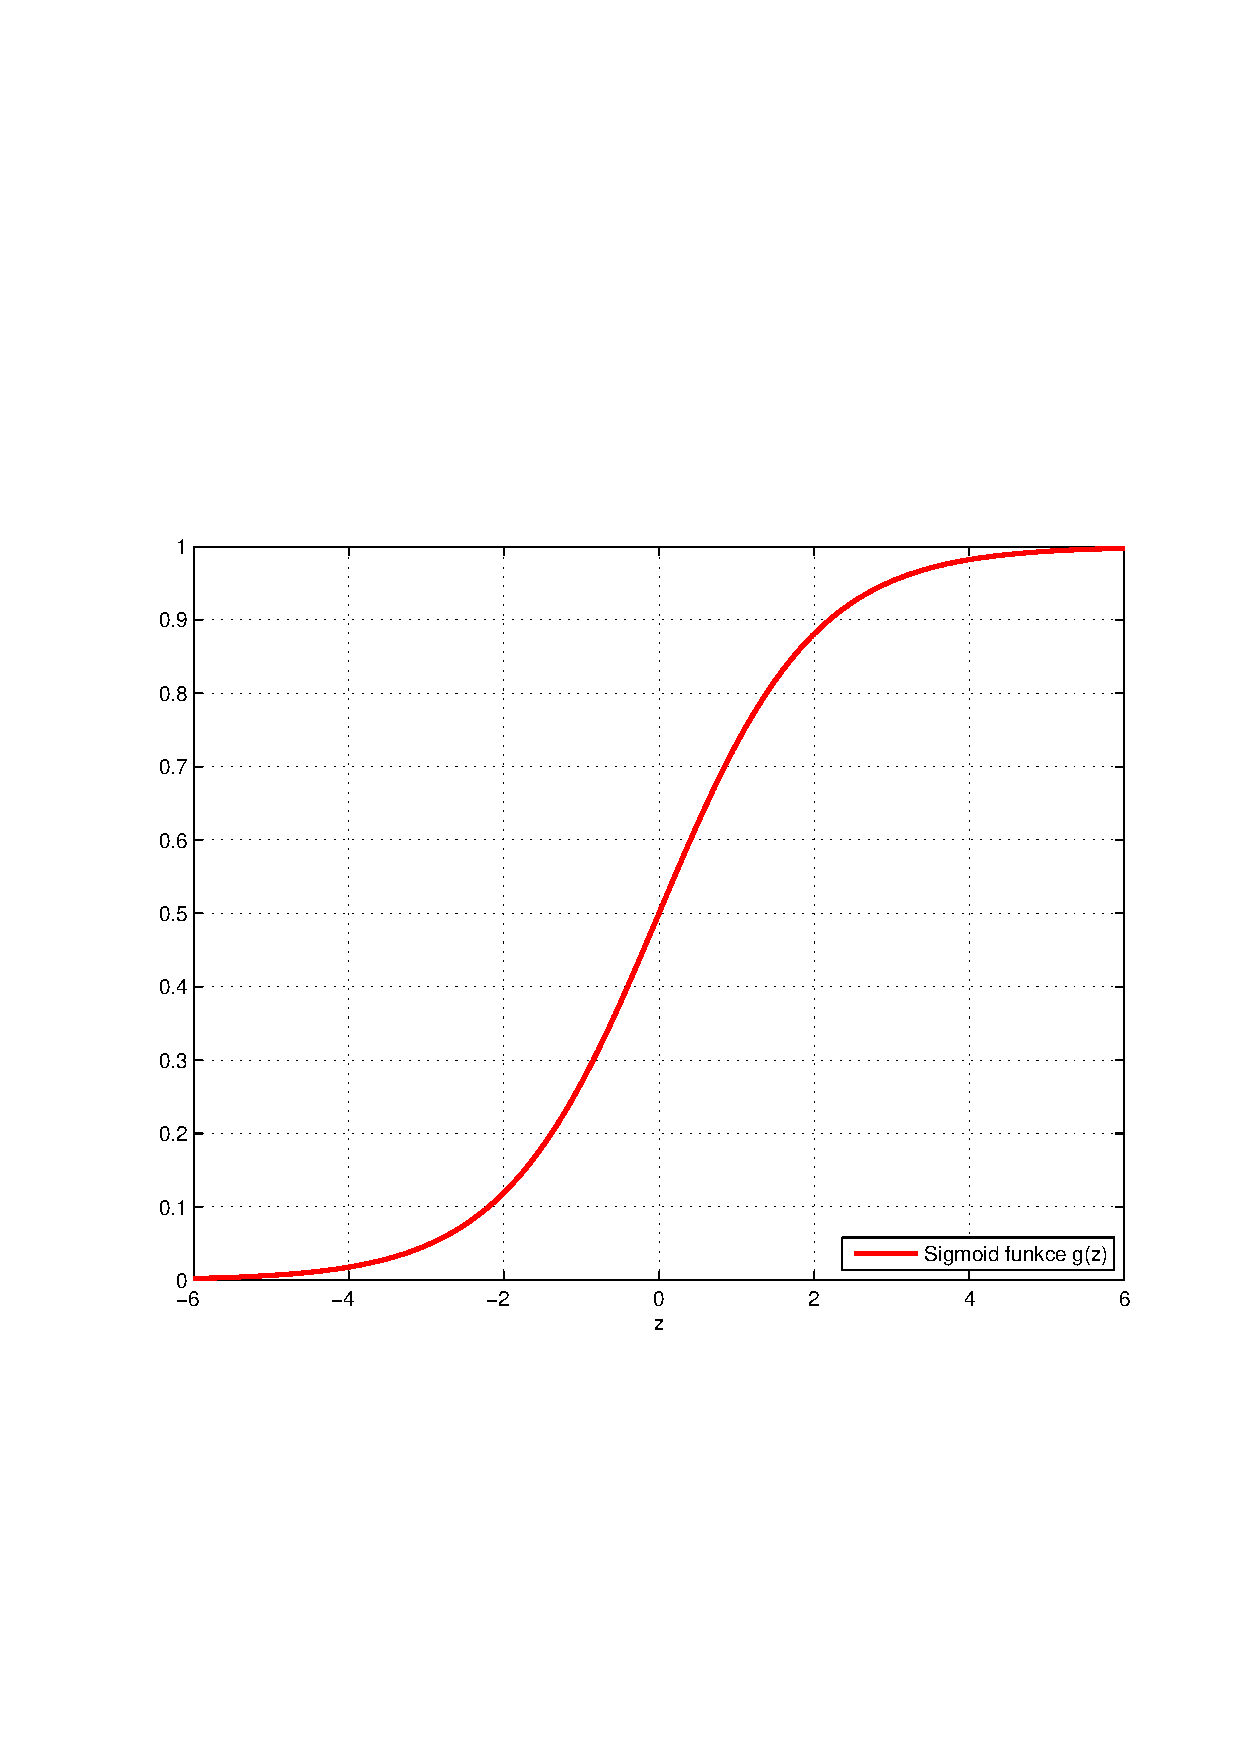
\includegraphics[width = 0.48\textwidth, trim = 2.5cm 7cm 2cm 9cm]{./Img/BinarniRegrese/sigmoidFunkce/sigmoidFunction.pdf}
	\caption{Sigmoidní funkce $g \left( z \right)$.}
	\label{fig:sigmoidFunction}
\end{figure}}
\par{Poznamenejme, že
\begin{eqnarray}
	\nonumber
	\lim_{z \to +\infty} &g \left( z \right) &= 1,\\
	\nonumber
	\lim_{z \to -\infty} &g \left( z \right) &= 0.
\end{eqnarray}}

\par{Nyní je potřeba, stejně jako dříve, přizpůsobit parametry $\bm{\Theta}$ našim datům, tedy pomocí trénovací množiny zvolit hodnoty parametrů $\bm{\Theta}$ a využít tyto parametry pro výpočet predikce.}

\par{Dále si povíme něco o interpretaci výstupu hypotézy. Hypotéza $h_{\bm{\Theta}} \left( \bm{x} \right) = $ odhadnutá pravděpodobnost, že výstup $y = 1$ na základě vstupních dat $\bm{x}$.}

\subsubsection*{Příklad}
\par{Pokud $\bm{x} = [ x_0,~x_1 ]^{\top} = [ 1,~$velikost nádoru$]^{\top}$ a $h_{\bm{\Theta}} \left( \bm{x} \right) = 0.7$, což říká pacientovi, že šance, že je nádor zhoubný je $70\%$. Nyní naše tvrzení zapíšeme formálněji
\begin{equation}
	h_{\bm{\Theta}} \left( \bm{x} \right) = P \left( y = 1 | \bm{x} ; \bm{\Theta} \right),
\end{equation}
neboli, pravděpodobnost, že $y = 1$, \uv{na základě dat $\bm{x}$}, parametrizovaná parametry $\bm{\Theta}$. V případě klasifikace víme, že výstup $y$ může nabývat pouze hodnot 0 nebo 1, proto platí
\begin{equation}
	P \left( y = 0 | \bm{x} ; \bm{\Theta} \right) + P \left( y = 1 | \bm{x} ; \bm{\Theta} \right) = 1,
\end{equation}
neboli
\begin{equation}
	P \left( y = 0 | \bm{x} ; \bm{\Theta} \right) = 1 - P \left( y = 1 | \bm{x} ; \bm{\Theta} \right).
\end{equation}}

\subsubsection*{Poznámka}
\par{Pravděpodobnost může nabývat hodnot $0-1$, neboli $0-100\%$.}





\newpage












%----------ROZHODOVACI-HRANICE-------------------------------------------------------------
\subsection{Rozhodovací hranice}
\label{sec:BinarniRegreseRozhodovaciHranice}

\par{V~této kapitole si povíme něco o~rozhodovací hranici, abychom získali větší ponětí o~výpočtu hypotézy binární regrese (klasifikace).}

\par{V kapitole \ref{sec:BinarniRegreseReprezentaceHypotezy} jsme si ukázali tvar hypotézy (sigmoid funkce)
\begin{equation}
	h_{\bm{\Theta}} \left( \bm{x} \right) = g \left( \bm{\Theta}^{\top} \bm{x} \right),
\end{equation}
kde
\begin{equation}
	g \left( \bm{z} \right) = \frac{1}{1 + e^{-\bm{z}}}
\end{equation}
a graf lze vidět na Obr. \ref{fig:sigmoidFunction2}.
\begin{figure}[!ht]
	\centering
	%trim option's parameter order: left bottom right top
	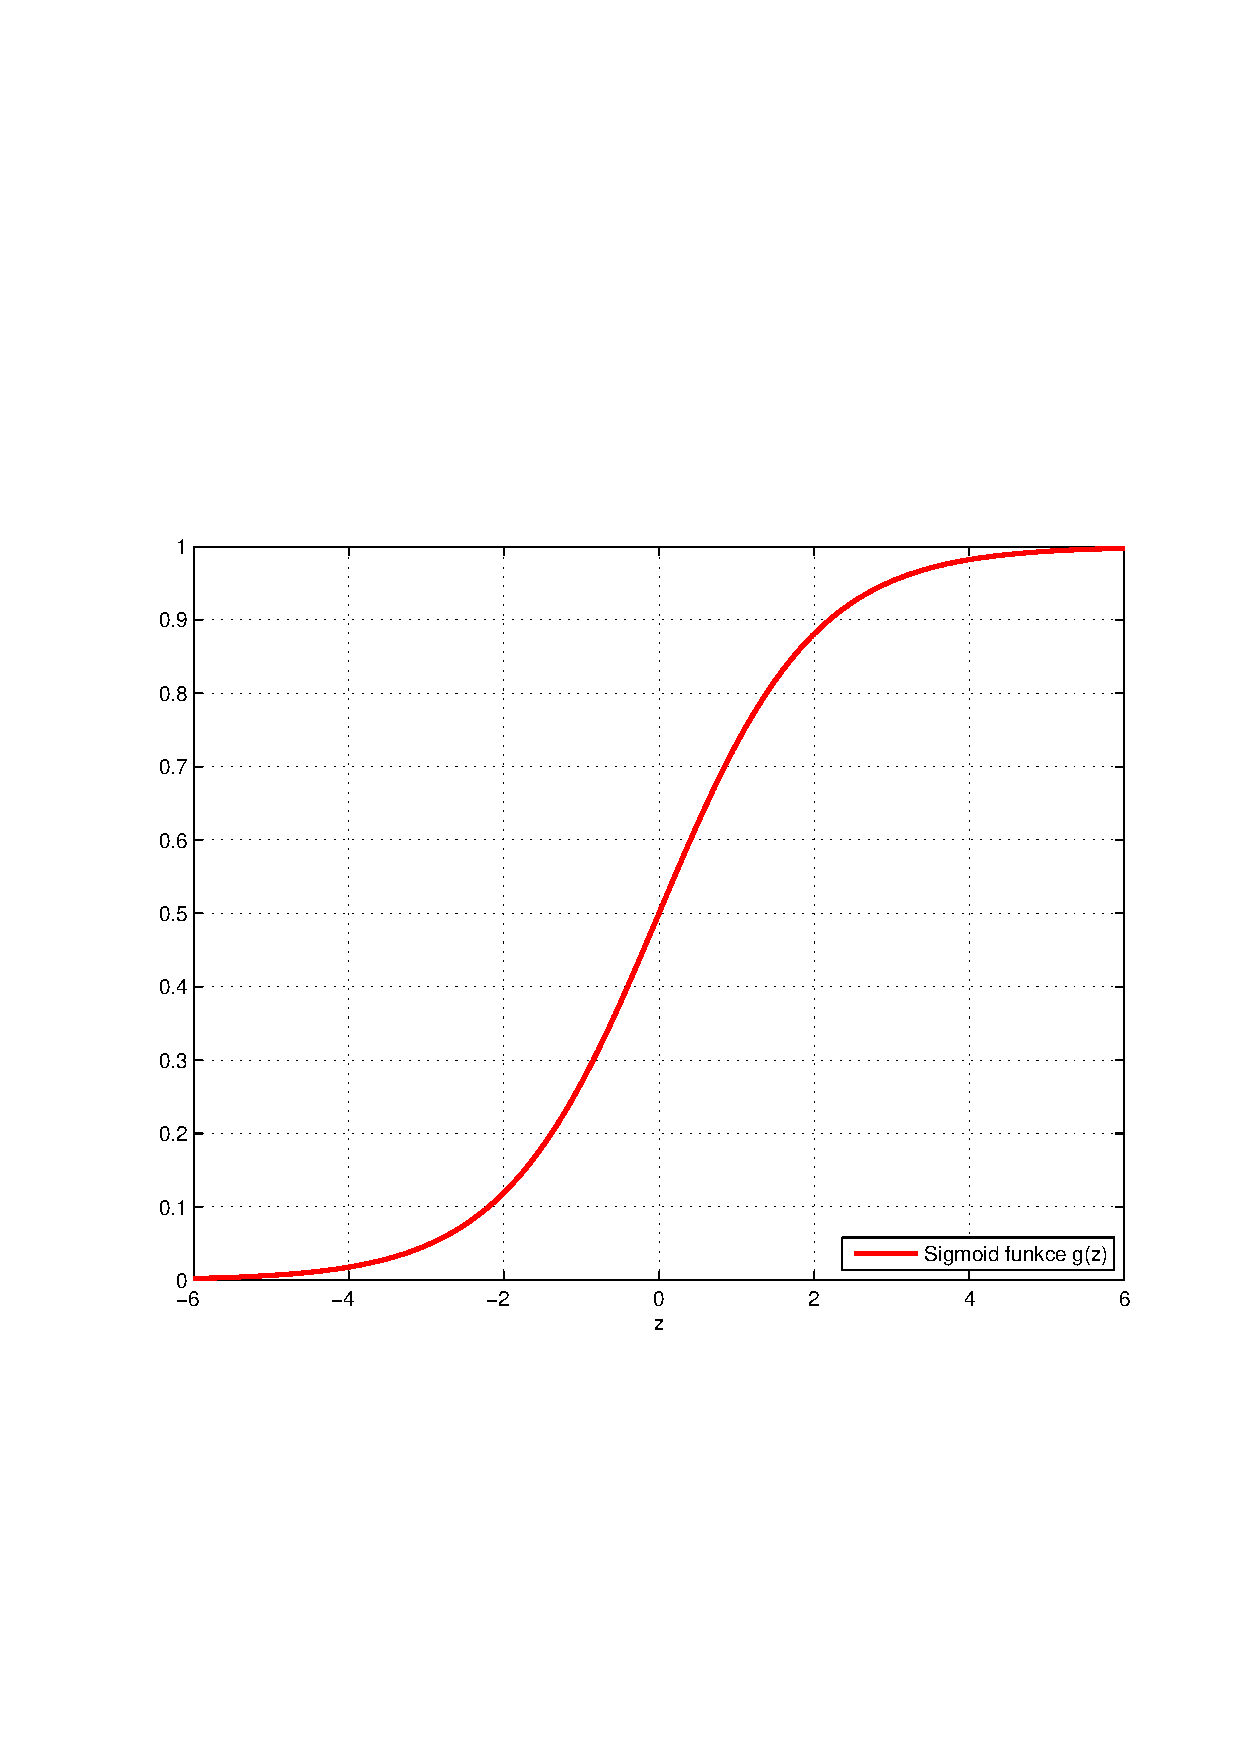
\includegraphics[width = 0.48\textwidth, trim = 2.5cm 7cm 2cm 9cm]{./Img/BinarniRegrese/sigmoidFunkce/sigmoidFunction.pdf}
	\caption{Sigmoidní funkce $g \left( z \right)$.}
	\label{fig:sigmoidFunction2}
\end{figure}}

\par{Podrobněji vysvětlíme, kdy naše hypotéza bude predikovat na výstupu 0 nebo 1. Konkrétně naše hypotéza bude na výstupu predikovat $y = 1$ v případě
\begin{equation}
	h_{\bm{\Theta}} \left( \bm{x} \right) = g \left( \bm{\Theta}^{\top} \bm{x} \right) = P \left( y = 1 | \bm{x}; \bm{\Theta} \right).
\end{equation}
Předpokládejme, že klasifikátor predikuje výstup $y = 1$ pokud $h_{\bm{\Theta}} \left( \bm{x} \right) \geq 0.5$, což platí pro $\bm{\Theta}^{\top} \bm{x} \geq 0$ a~klasifikátor predikuje výstup $y = 0$ pokud $h_{\bm{\Theta}} \left( \bm{x} \right) < 0.5$, což platí pro $\bm{\Theta}^{\top} \bm{x} < 0$.}

\newpage

\subsubsection*{Příklad - lineárně separabilní třídy}
\par{Předpokládejme, že máme trénovací sadu, která je znázorněna na Obr.~\ref{fig:decisionBoundary1} a~naše hypotéza má tvar
\begin{equation}
	h_{\bm{\Theta}} \left( \bm{x} \right) = g \left( \vartheta_0 + \vartheta_1 x_1 + \vartheta_2 x_2 \right).
	\label{eq:linearniHypotezaRovnice}
\end{equation}
Nyní se nebudeme zabývat tím, jak přizpůsobit parametry tomuto modelu. Předpokládejme, že $\bm{\Theta} = \left[ \vartheta_0,~\vartheta_1,~\vartheta2 \right]^{\top} = \left[ -3,~1,~1 \right]^{\top}$.}
\begin{figure}[!ht]
	\centering
	\begin{minipage}[t]{0.48\textwidth}
		%trim option's parameter order: left bottom right top
		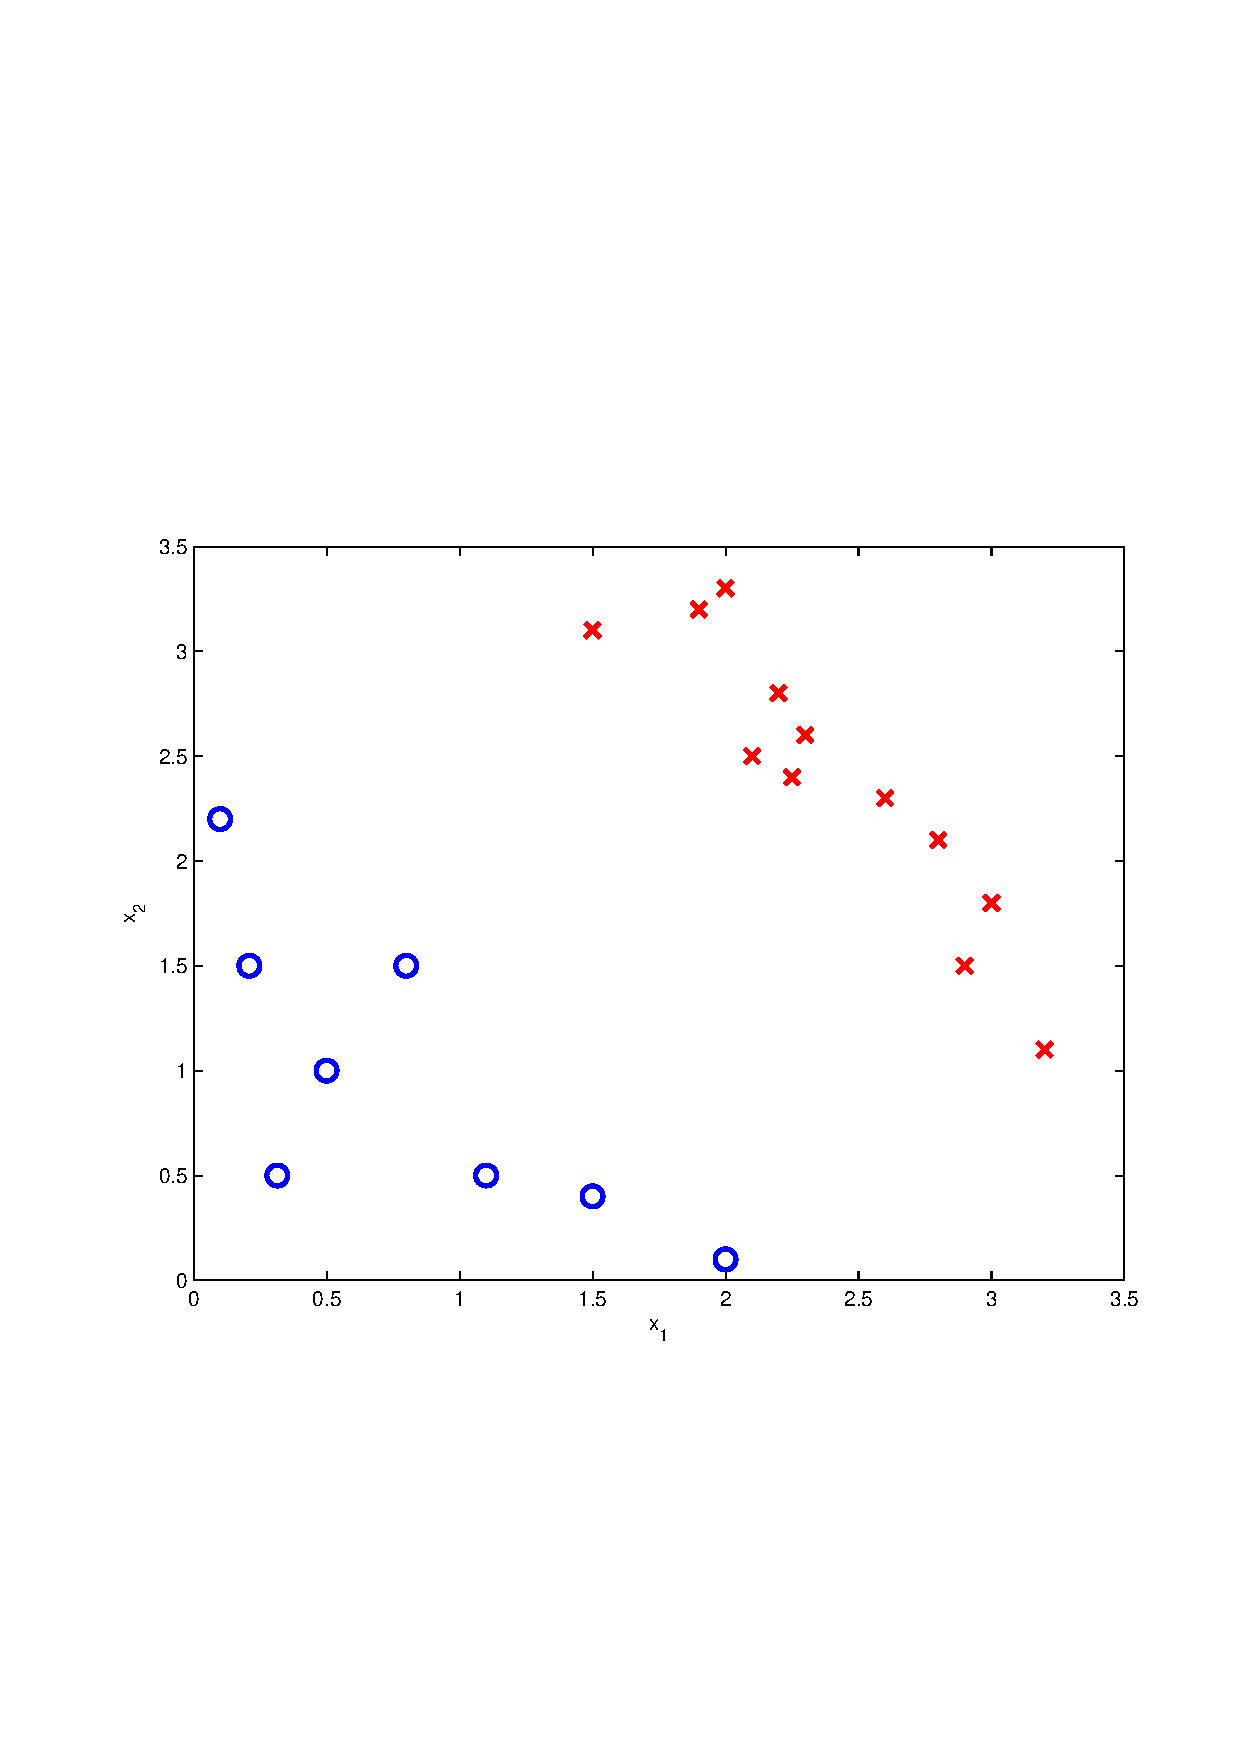
\includegraphics[width = \textwidth, trim = 2.5cm 7cm 2cm 9cm]{./Img/BinarniRegrese/decisionBoundary/decisionBoundary1.pdf}
		\caption{Vizualizace dvou tříd.}
		\label{fig:decisionBoundary1}
	\end{minipage}%
	\hfill
	\begin{minipage}[t]{0.48\textwidth}
		%trim option's parameter order: left bottom right top
		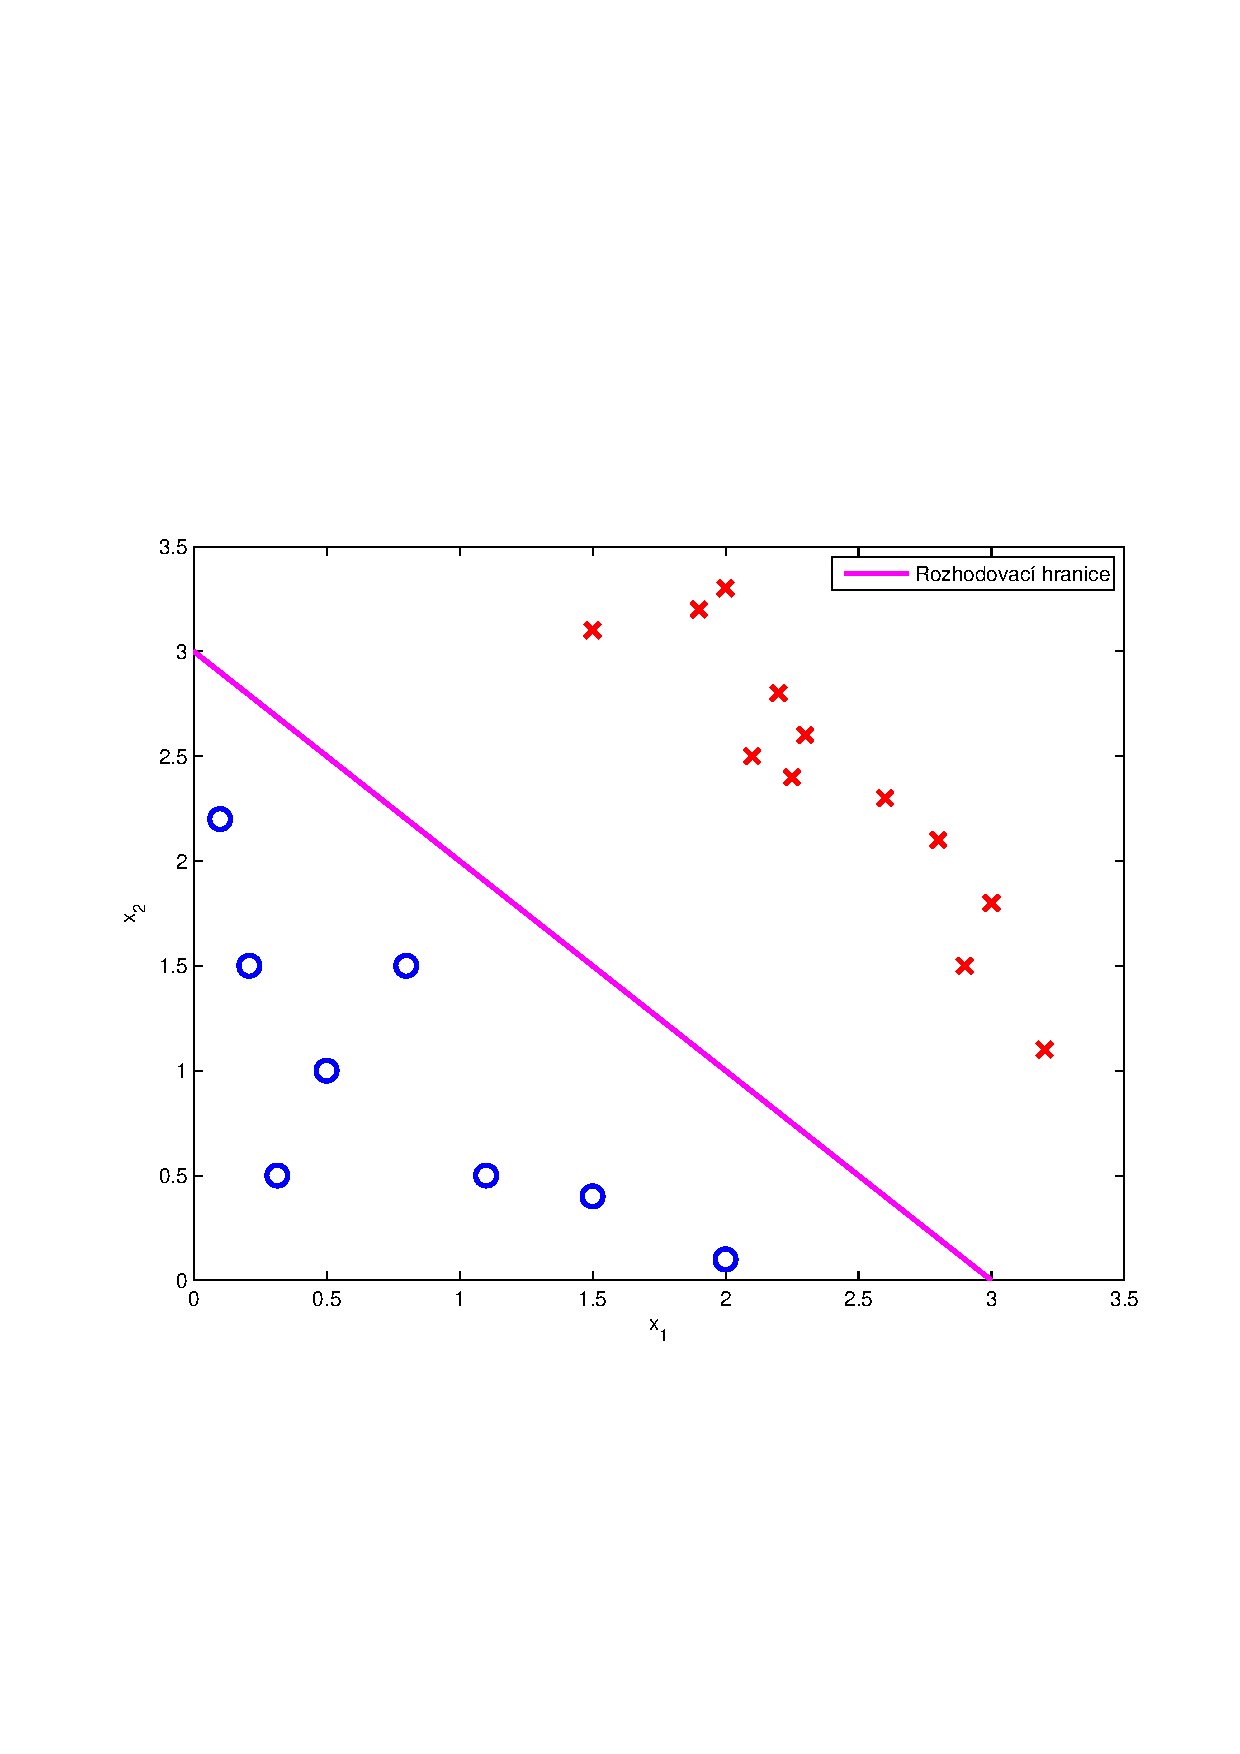
\includegraphics[width = \textwidth, trim = 2.5cm 7cm 2cm 9cm]{./Img/BinarniRegrese/decisionBoundary/decisionBoundary2.pdf}
		\caption{Vizualizace rozhodovací hranice.}
		\label{fig:decisionBoundary2}
	\end{minipage}%
\end{figure}

\par{Na příkladu si ukážeme, kdy hypotéza bude predikovat, jako výstup 0 a kdy 1. Hypotéza bude predikovat výstupní hodnotu $y = 1$ pokud
\begin{equation}
	-3 + x_1 + x_2 \geq 0
	\label{eq:prikladDecisionBoundary}
\end{equation}
($\bm{\Theta}^{\top} \bm{x} \geq 0$), jinými slovy pro všechna $x_1$ a $x_2$, které splňují rovnici \ref{eq:prikladDecisionBoundary} bude naše hypotéza predikovat výstup $y = 1$. Řešení rovnice \ref{eq:prikladDecisionBoundary} je naznačeno na Obr. \ref{fig:decisionBoundary2} a~odpovídají mu červené křížky nad rozhodovací hranicí.}

\par{V~případě, kdy $x_1 + x_2 = 3$, tak to odpovídá přesně $h_{\bm{\Theta}} \left( \bm{x} \right) = 0.5$. Jinak řečeno řešení odpovídá přesně rozhodovací hranici mezi třídami.}

\newpage

\subsubsection*{Příklad - lineárně neseparabilní třídy}
\par{Předpokládejme složitější příklad, kde nelze jednoduše použít binární regresi (lineární rozhodovací hranici) a~musíme využít polynomiální regrese, tedy musíme využít vyšší stupně polynomů jako příznaky viz Obr. \ref{fig:decisionBoundary3}.}
\begin{figure}[!ht]
	\centering
	\begin{minipage}[t]{0.48\textwidth}
		%trim option's parameter order: left bottom right top
		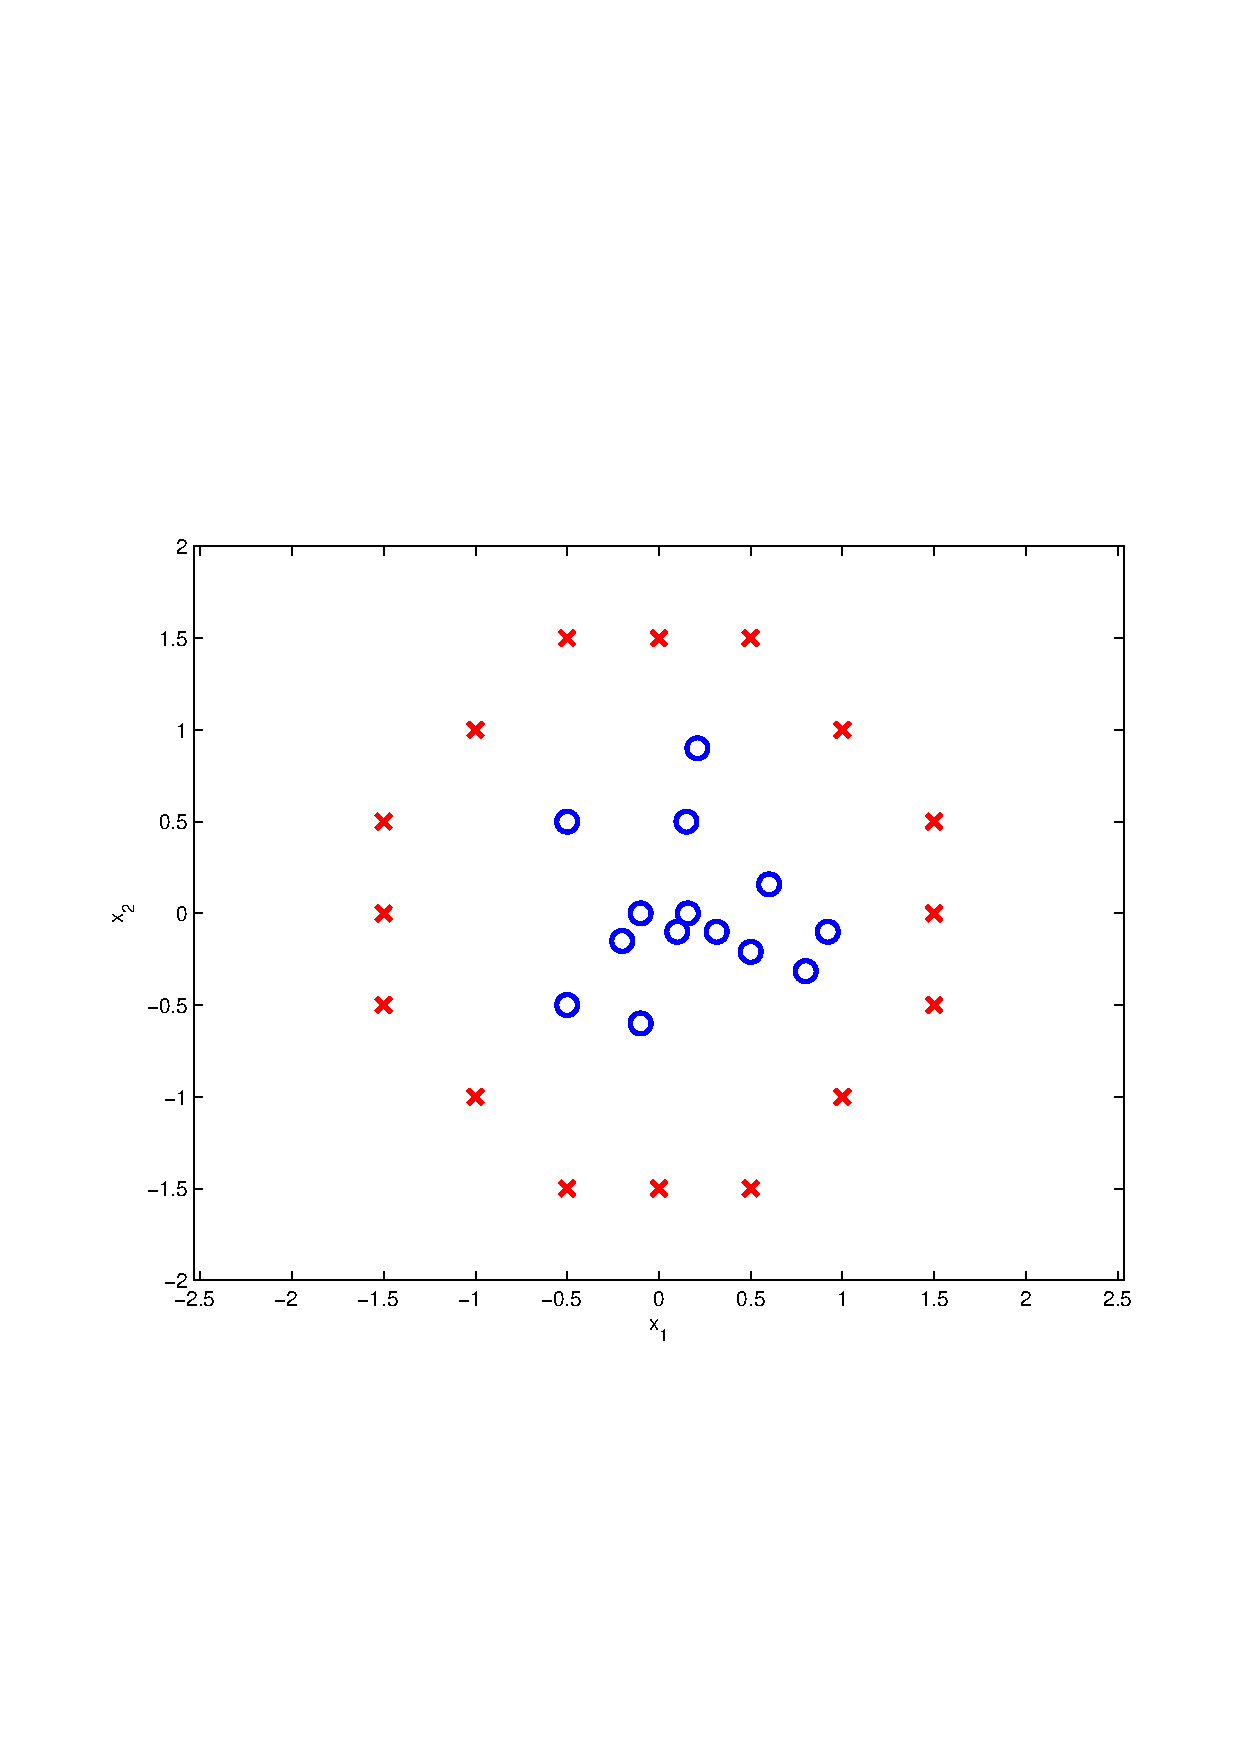
\includegraphics[width = \textwidth, trim = 2.5cm 7cm 2cm 9cm]{./Img/BinarniRegrese/decisionBoundary/decisionBoundary3.pdf}
		\caption{Vizualizace lineárně neseparabilních tříd.}
		\label{fig:decisionBoundary3}
	\end{minipage}%
	\hfill
	\begin{minipage}[t]{0.48\textwidth}
		%trim option's parameter order: left bottom right top
		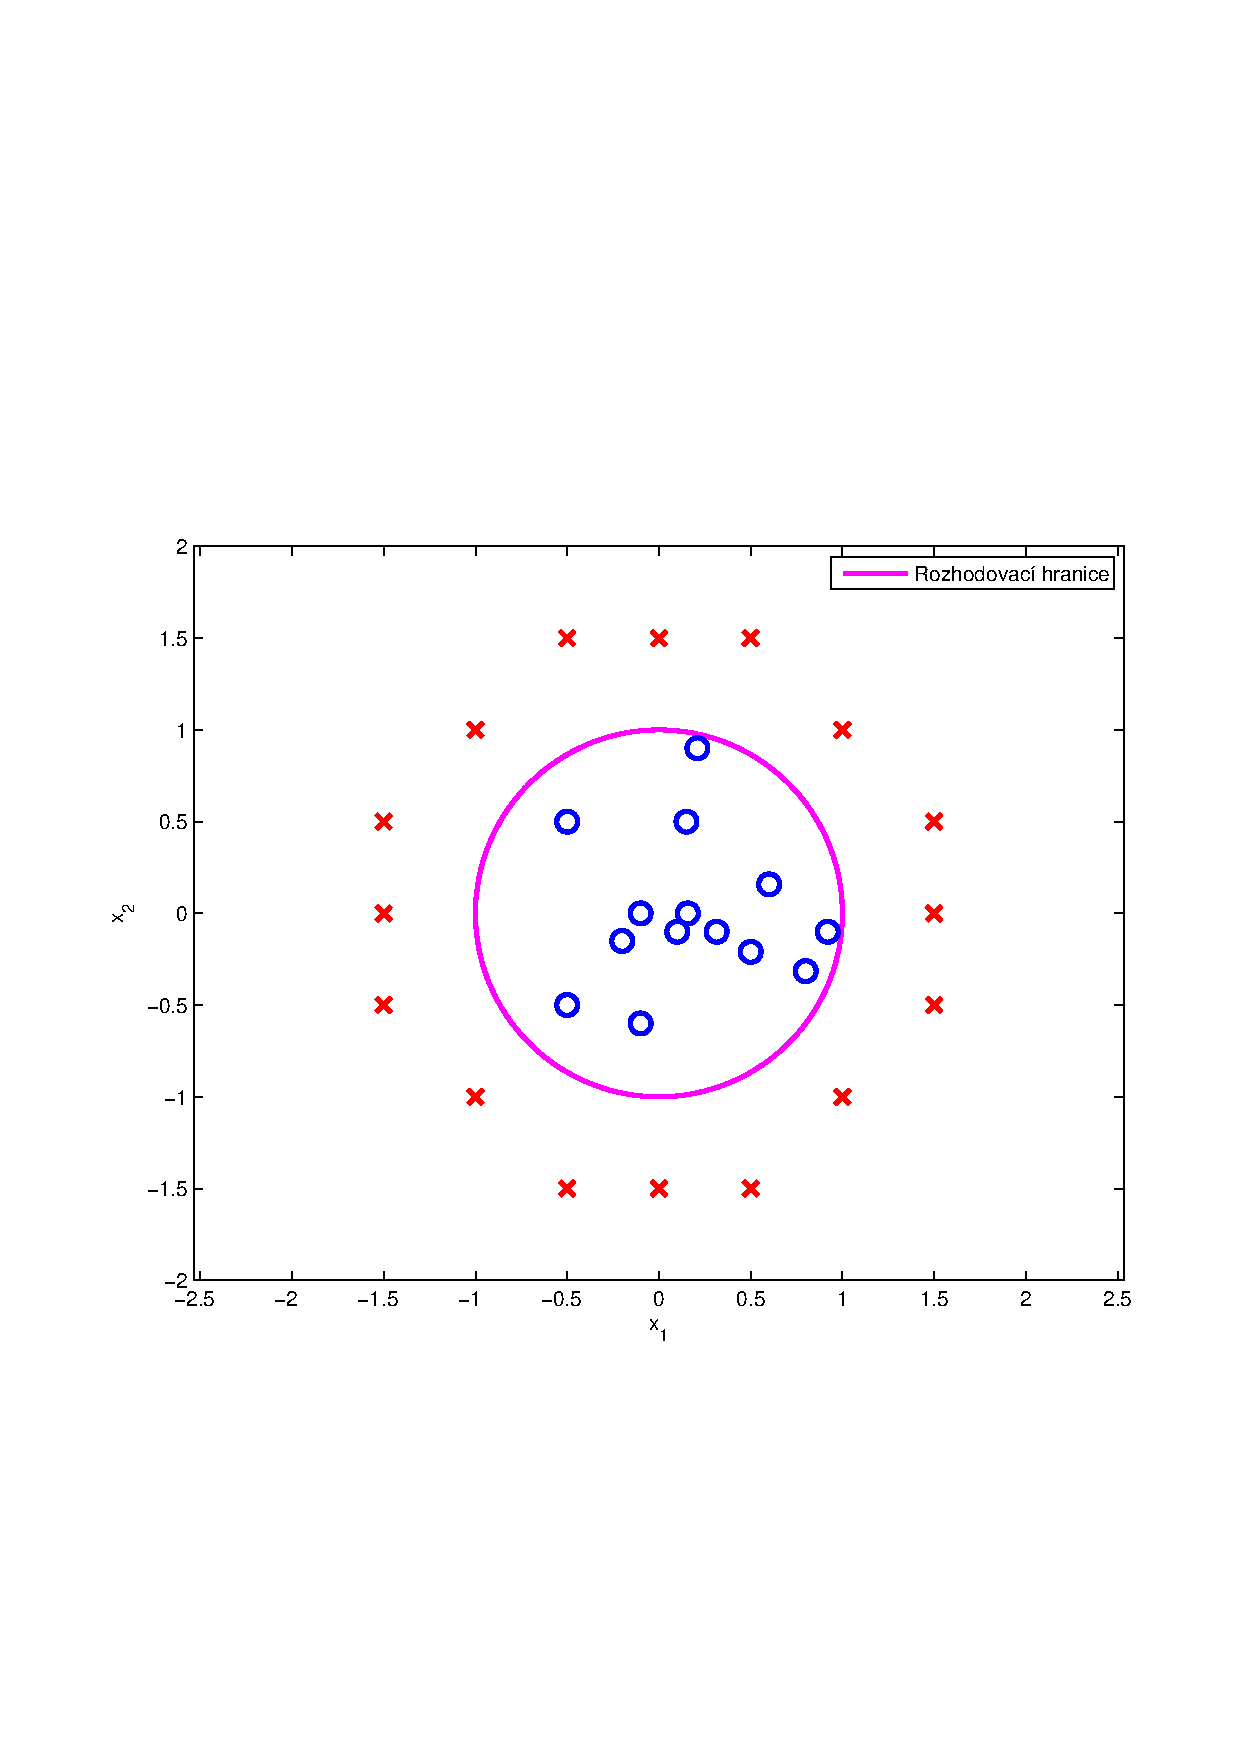
\includegraphics[width = \textwidth, trim = 2.5cm 7cm 2cm 9cm]{./Img/BinarniRegrese/decisionBoundary/decisionBoundary4.pdf}
		\caption{Vizualizace lineárně neseparabilních tříd společně s~rozhodovací hranicí.}
		\label{fig:decisionBoundary4}
	\end{minipage}%
\end{figure}

\par{Naše hypotéza má tvar $h_{\bm{\Theta}} \left( \bm{x} \right) = g \left( \vartheta_0 + \vartheta_1 x_1 + \vartheta_2 x_2 + \vartheta_3 x_1^2 + \vartheta_4 x_2^2 \right)$, kde jsme oproti předcházejícímu příkladu (rovnice \ref{eq:linearniHypotezaRovnice}) přidali dva příznaky $x_1^2$ a $x_2^2$ a~máme 5~parametrů $\vartheta_{0,\ldots,4}$. Nebudeme zabývat tím, jak vypočítat parametry $\bm{\Theta}$ (bude popsáno v~následujících sekcích), řekněme, že $\bm{\Theta} = \left[ \vartheta_0,~\vartheta_1,~\vartheta_2,~\vartheta_3,~\vartheta_4 \right]^{\top} = \left[ -1,~0,~0,~1,~1 \right]^{\top}$. Což znamená, že naše hypotéza bude predikovat výstup $y = 1$ pokud $-1 + x_1^2 + x_2^2 \geq 0$ (pro směr ven od rozhodovací hranice), tato rovnice odpovídá rovnici kružnice $x_1^2 + x_2^2 = 1$ o~poloměru $r = 1$. Rozhodovací hranice je vidět na Obr.~\ref{fig:decisionBoundary4}.}

\subsubsection*{Poznámka}
\par{Rozhodovací hranice je vlastnost hypotézy, konkrétně parametrů $\bm{\Theta}$, není to vlastnost trénovací sady. Trénovací sada je pouze využita k nalezení parametrů hypotézy~$\bm{\Theta}$.}





\newpage















%----------------------------------------------------------------------------------------
\subsection{Ztrátová funkce}
\label{sec:BinarniRegreseZtratovaFunkce}

\par{V této sekci si povíme jak vypočítat parametry $\bm{\Theta}$ pro binární regresi / klasifikaci.}

\par{Definujme problém učení s učitelem pro binární regresní model. Mějme trénovací množinu
\begin{equation}
	\{ \left( \bm{x}^{\left( 1 \right)}, y^{\left( 1 \right)} \right), \left( \bm{x}^{\left( 2 \right)}, y^{\left( 2 \right)} \right), \ldots , \left( \bm{x}^{\left( m \right)}, y^{\left( m \right)} \right) \}
\end{equation}
o velikosti $m$ vzorků, kde
\begin{equation}
	\bm{x}^{\left( i \right)} = \left[ x_0,~x_1,~\ldots,~x_n \right]^{\top},
\end{equation}
$\bm{x}^{\left( i \right)} \in \mathrm{R}^{n+1}$ a $x_0 = 1$, $y \in \{ 0,1 \}$. Naše hypotéza má tvar
\begin{equation}
	h_{\bm{\Theta}} \left( \bm{x} \right) = \frac{1}{1 + e^{-\bm{\Theta}^{\top} \bm{x}}}.
\end{equation}}

\par{Nyní si položme zásadní otázku, jak zvolit parametry $\bm{\Theta}$ v závislosti na naší trénovací množině?}

\par{Připomeňme si ztrátovou funkci $J \left( \bm{\Theta} \right)$ pro lineární regresi (viz sekce \ref{sec:LinearniRegreseZtratovaFunkce}), kterou zapíšeme v následujícím tvaru
\begin{equation}
	J \left( \bm{\Theta} \right) = \frac{1}{m} \sum_{i=1}^{m} \frac{1}{2} \left( h_{\Theta} \left( \bm{x}^{\left( i \right)} \right) - y^{\left( i \right)} \right)^2,
\end{equation}
dále můžeme ztrátovou funkci přepsat do tvaru
\begin{equation}
	J \left( \bm{\Theta} \right) = \frac{1}{m} \sum_{i=1}^{m} Cena \left( h_{\bm{\Theta}} \left( \bm{x}^{\left( i \right)} \right), y^{\left( i \right)} \right),
	\label{eq:JcenaX}
\end{equation}
kde
\begin{equation}
	Cena \left( h_{\bm{\Theta}} \left( \bm{x}^{\left( i \right)} \right), y^{\left( i \right)} \right) = \frac{1}{2} \left( h_{\bm{\Theta}} \left( \bm{x}^{\left( i \right)} \right) - y^{\left( i \right)} \right)^2.
	\label{eq:cenaX}	
\end{equation}
Nyní lze z rovnice \ref{eq:JcenaX} lépe vidět, že ztrátová funkce je $\frac{1}{m}$ krát součet $Cen$ přes trénovací sadu. Rovnici \ref{eq:cenaX} lze dále zjednodušit vynecháním horních indexů
\begin{equation}
	Cena \left( h_{\bm{\Theta}} \left( \bm{x} \right), y \right) = \frac{1}{2} \left( h_{\Theta} \left( \bm{x} \right) - y \right)^2
\end{equation}
a říká nám jakou $Cenu$ zaplatíme pokud výstupní hodnota hypotézy bude $h_{\bm{\Theta}} \left( \bm{x} \right)$ a výstupní informace od učitele bude hodnota $y$.}

\par{Tento předpis \ref{eq:cenaX} pro výpočet $Ceny$ platí pro lineární regresi. Avšak v této sekci se zajímáme o binární regresi. Pokud bychom chtěli minimalizovat tuto ztrátovou funkci v rovnici \ref{eq:JcenaX}, tak tato funkce může být nekonvexní vzhledem k parametrům $\bm{\Theta}$ (není zaručeno, že dosáhneme globálního minima, jako v případě konvexní ztrátové funkce).}

\par{Uveďme si ztrátovou funkci, která se využívá při binární regresi
\begin{equation}
	\label{eq:ztratovaFunkceBinarniRegrese}
	Cena \left( h_{\bm{\Theta}} \left( \bm{x} \right), y \right) = \left\{
	\begin{array}{r}
		{- \log \left( h_{\bm{\Theta}} \left( \bm{x} \right) \right), \quad \textrm{pro}~y = 1} \\
		{- \log \left( 1 - h_{\bm{\Theta}} \left( \bm{x} \right) \right), \quad \textrm{pro}~y = 0}
	\end{array}
	\right.
\end{equation}
jinými slovy lze říci, že se jedná jakou ztrátu (kolik nás stojí) utrpíme pokud $y = 0$ nebo $y = 1$.}


\newpage

\par{Nyní si ztrátovou funkci pro binární regresi, z rovnice \ref{eq:ztratovaFunkceBinarniRegrese}, rozebereme podrobněji. Na Obr. \ref{fig:ztratovaFunkce3} lze vidět průběh ztrátové funkce.
\begin{figure}[!ht]
	\centering
	%trim option's parameter order: left bottom right top
	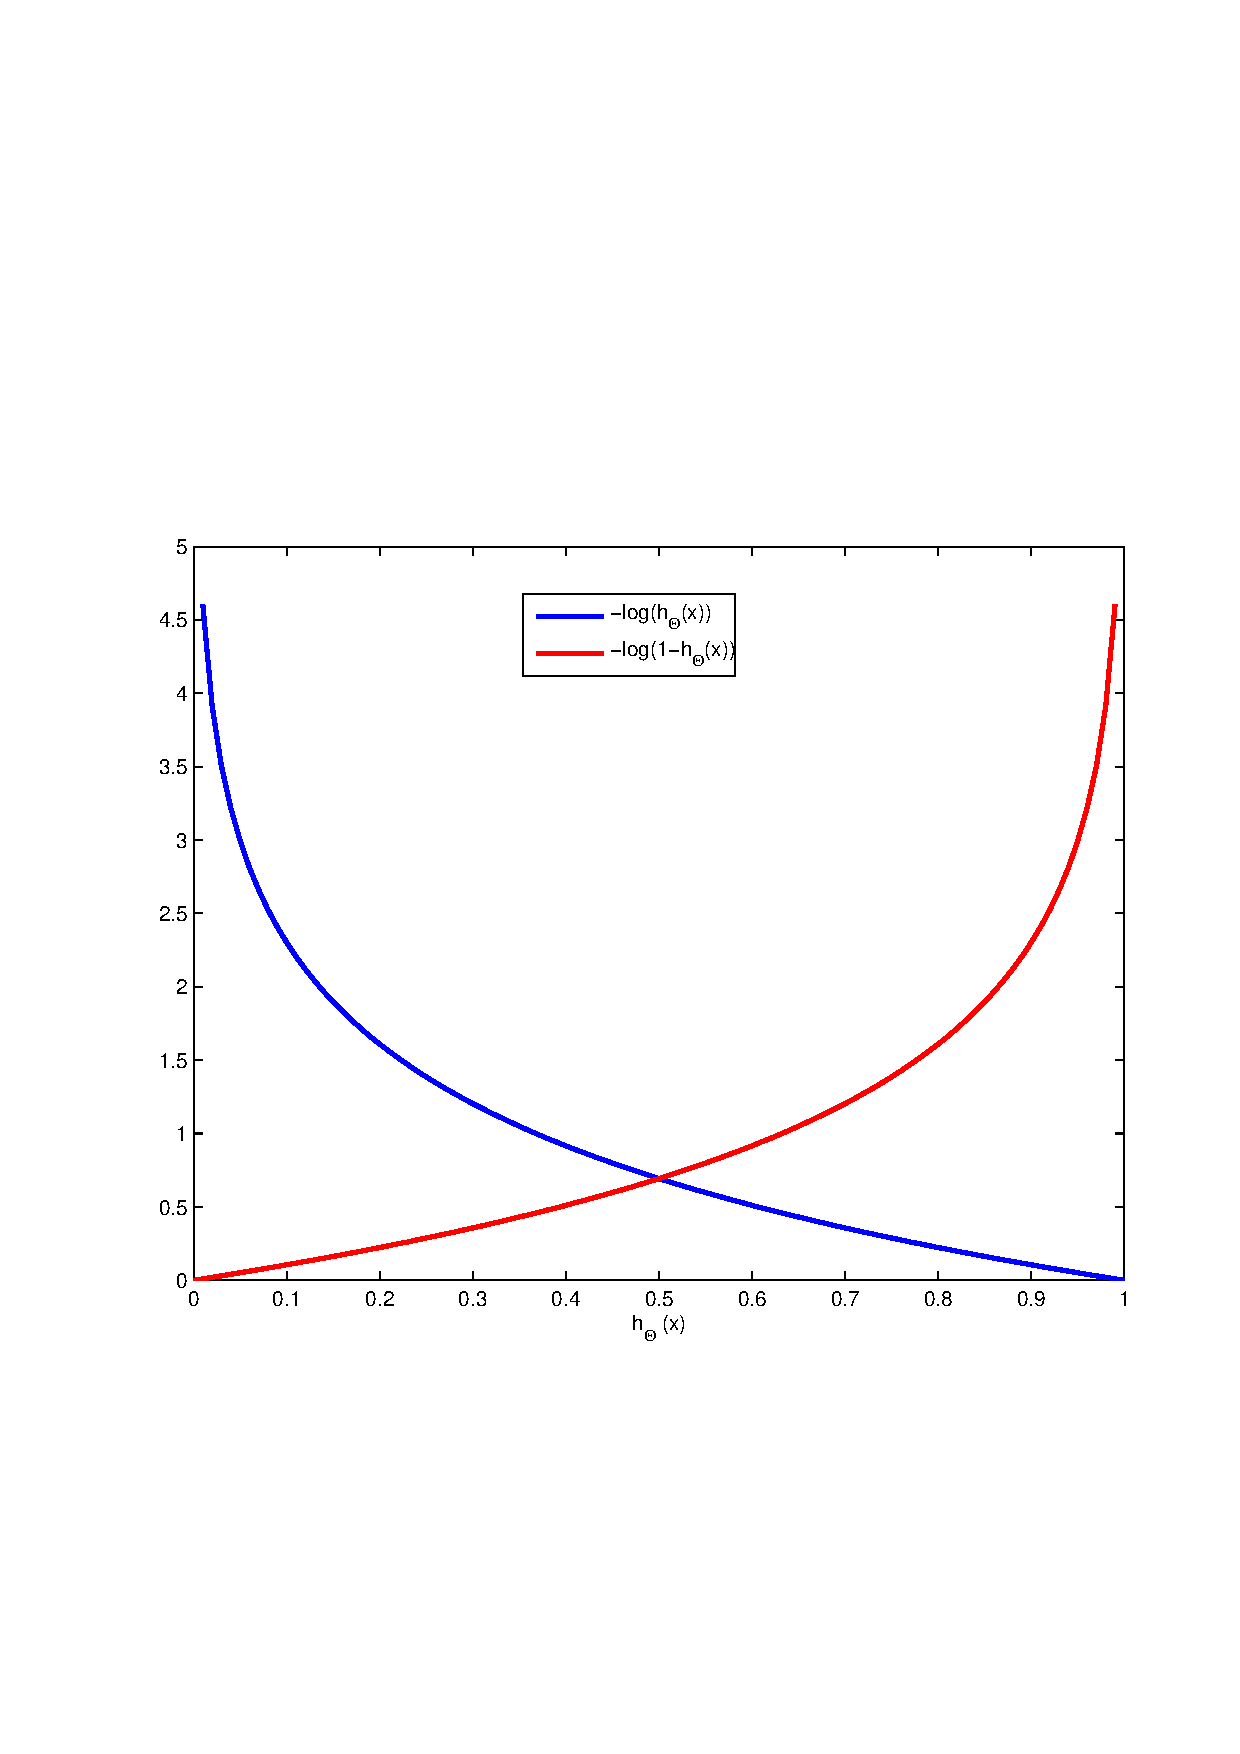
\includegraphics[width = 0.48\textwidth, trim = 2.5cm 7cm 2cm 9cm]{./Img/BinarniRegrese/ztratovaFunkce/ztratovaFunkce3.pdf}
	\caption{Průběh ztrátové funkce.}
	\label{fig:ztratovaFunkce3}
\end{figure}}

\par{Pokud bude $y = 1$ a naše hypotéza $h_{\bm{\Theta}} \left( \bm{x} \right) = 1$, tak utrpíme ztrátu rovnu $Cena = 0$. Ale pokud se bude hodnota hypotézy zmenšovat $h_{\bm{\Theta}} \left( \bm{x} \right) \rightarrow 0$, tak se utrpěná ztráta bude zvětšovat $Cena \rightarrow \infty$. V druhém případě pokud $h_{\bm{\Theta}} \left( \bm{x} \right) = 0$ (predikce $P \left( y = 1 | \bm{x}; \bm{\Theta} \right) = 0$), ale $y = 1$, tak utrpěná ztráta bude velmi velká.}

\par{Pro $y = 0$ platí obdobně druhá část rovnice \ref{eq:ztratovaFunkceBinarniRegrese}.}





















%----------------------------------------------------------------------------------------
\subsection{Zjednodušená ztrátová funkce a gradientní metoda}

\par{Naše ztrátová funkce $J \left( \bm{\Theta} \right)$ ve tvaru
\begin{equation}
	J \left( \bm{\Theta} \right) = \frac{1}{m} \sum_{i=1}^{m} Cena \left( h_{\bm{\Theta}} \left( \bm{x}^{\left( i \right)} \right), y^{\left( i \right)} \right),
	\label{eq:JcenaXpodruhe}
\end{equation}
kde
\begin{equation}
	\label{eq:ztratovaFunkceBinarniRegrese2}
	Cena \left( h_{\bm{\Theta}} \left( \bm{x} \right), y \right) = \left\{
	\begin{array}{r}
		{- \log \left( h_{\bm{\Theta}} \left( \bm{x} \right) \right), \quad \textrm{pro}~y = 1} \\
		{- \log \left( 1 - h_{\bm{\Theta}} \left( \bm{x} \right) \right), \quad \textrm{pro}~y = 0}
	\end{array}
	\right.
\end{equation}
poznamenejme že $y = 0$ nebo $y = 1$ (pokaždé, žádná jiná možnost není).}

\par{Naší $Cenu$ z rovnice \ref{eq:ztratovaFunkceBinarniRegrese2} můžeme zapsat v jedné rovnici, která má tvar
\begin{equation}
	Cena \left( h_{\bm{\Theta}} \left( \bm{x} \right), y \right) = - y \log \left( h_{\bm{\Theta}} \left( \bm{x} \right) \right) - \left( 1 - y \right) \log \left( 1 - h_{\bm{\Theta}} \left( \bm{x} \right) \right),
	\label{eq:cena1rovnice}
\end{equation}
pokud $y = 1$, tak rovnice \ref{eq:cena1rovnice} přechází na první část rovnice \ref{eq:ztratovaFunkceBinarniRegrese2} a pokud $y = 0$, tak rovnice \ref{eq:cena1rovnice} přechází na druhou část rovnice \ref{eq:ztratovaFunkceBinarniRegrese2}.}

\par{Po spojení a úpravě rovnic \ref{eq:cena1rovnice} a \ref{eq:JcenaXpodruhe} získáme výsledný tvar
\begin{equation}
		J \left( \bm{\Theta} \right) = - \frac{1}{m} \left[ \sum_{i=1}^{m} y^{\left( i \right)} \log \left( h_{\bm{\Theta}} \left( \bm{x}^{\left( i \right)} \right) \right) + \left( 1 - y^{\left( i \right)} \right) \log \left( 1 - h_{\bm{\Theta}} \left( \bm{x}^{\left( i \right)} \right) \right) \right].
		\label{eq:ztratovaFunkceJbinarniRegrese}
\end{equation}}

\par{Cílem je nalézt takové parametry $\bm{\Theta}$, které minimalizují ztrátovou funkci $J$
\begin{equation}
	\min_{\bm{\Theta}} J \left( \bm{\Theta} \right),
\end{equation}
a následně pro vypočítáme predikci naší hypotézy (na základě nového vstupu $x$) 
\begin{equation}
	h_{\bm{\Theta}} \left( \bm{x} \right) = \frac{1}{1 + e^{ - \bm{\Theta}^{\top} \bm{x}}}.
\end{equation}}

\par{Nyní můžeme konečně zapsat celý gradientní algoritmus, opakuj
\begin{equation}
	\vartheta_j = \vartheta_j - \alpha \frac{\partial}{\partial \vartheta_j} J \left( \bm{\Theta} \right),
	\label{eq:gradientDescentBinaryRegresionAlgorithm}
\end{equation}
po každé iteraci aktualizuj všechny parametry $\vartheta_j$ najednou dokud algoritmus nedokonverguje.}

\subsubsection*{Poznámka}
\par{V rovnici \ref{eq:gradientDescentBinaryRegresionAlgorithm} bude využit tvar
\begin{equation}
	\frac{\partial}{\partial \vartheta_j} J \left( \bm{\Theta} \right) = \frac{1}{m} \sum_{i = 1}^{m} \left( h_{\bm{\Theta}} \left( \bm{x}^{\left( i \right)} \right) - y^{\left( i \right)} \right) \bm{x}_j^{\left( i \right)}.
\end{equation} a proto je výhodnější psát rovnici \ref{eq:gradientDescentBinaryRegresionAlgorithm} ve tvaru
\begin{equation}
		\vartheta_j = \vartheta_j - \alpha \sum_{i = 1}^{m} \left( h_{\bm{\Theta}} \left( \bm{x}^{\left( i \right)} \right) - y^{\left( i \right)} \right) \bm{x}_j^{\left( i \right)}.
\end{equation}}

\par{Algoritmus vypadá totožně jako v případě lineární regrese (viz \ref{eq:NDgradientDescentVysledna}) s rozdílnou hypotézou $h_{\bm{\Theta}} \left( \bm{x} \right)$, v případě lineární regrese
\begin{equation}
	h_{\bm{\Theta}} \left( \bm{x} \right) = \bm{\Theta}^{\top} \bm{x}
\end{equation}
a v případě binární regrese se jedná o
\begin{equation}
	h_{\bm{\Theta}} \left( \bm{x} \right) = \frac{1}{1 + e^{- \bm{\Theta}^{\top} \bm{x}}}.
\end{equation}}

\subsubsection*{Poznámka}
\par{Při výpočtu parametrů $\bm{\Theta}$ pomocí gradientního algoritmu v případě binární regrese je také vhodné využít Features scaling, jako v případě lineární regrese (viz sekce \ref{sec:featuresScaling}).}



\newpage



















%----------------------------------------------------------------------------------------
\subsection{Pokročilé algoritmy optimalizace}

\par{V této sekci si uvedeme příklady několika pokročilejších algoritmů optimalizace, které jsou lépe využitelné pro velké problémy strojového učení, kde je například velký počet příznaků.}

\par{Připomeňme náš optimalizační problém, máme ztrátovou funkci $J \left( \bm{\Theta} \right)$ a chceme jí minimalizovat
\begin{equation}
	\min_{\bm{\Theta}} J \left( \bm{\Theta} \right).
\end{equation}
Musíme tedy znát rovnice pro výpočet $J \left( \bm{\Theta} \right)$ a $\frac{\partial}{\partial \vartheta_j} J \left( \bm{\Theta} \right)$ následně můžeme využít zmíněný gradientní algoritmus, nebo nějakou z pokročilejších optimalizačních metod jako jsou například
\begin{table}[!ht]
\begin{center}
\begin{tabular}{r|c|c}
	{Název algoritmu} & {Výhody} & {Nevýhody}\\
	\hline
	{Conjugate gradient} & {Nemusí se volit} & {Více složité}\\
	{BFGS} & {konstanta učení $\alpha$.} & {}\\
	{L-BFGS} & {Rychlejší než gradientní metoda.} & {}
\end{tabular}
	\caption{Příklady pokročilejších optimalizačních algoritmů.}
\end{center}
\end{table}}

\subsubsection*{Příklad}
\par{Nyní si uvedeme příklad společně s jeho implementací v~MATLABu. Mějme vektor parametrů $\bm{\Theta} = \left[ \vartheta_1,~\vartheta_2 \right]^{\top}$ a ztrátovou funkci $J \left( \bm{\Theta} \right) = \left( \vartheta_1 - 5 \right)^2 + \left( \vartheta_2 - 5 \right)^2,$ dále vypočteme parciální derivace ztrátové funkce
\begin{eqnarray}
	\label{eq:prGrad1}
	\frac{\partial}{\partial \vartheta_1} &J \left( \bm{\Theta} \right) &= 2 \cdot \left( \vartheta_1 - 5 \right),\\
	\label{eq:prGrad2}
	\frac{\partial}{\partial \vartheta_2} &J \left( \bm{\Theta} \right) &= 2 \cdot \left( \vartheta_2 - 5 \right).
\end{eqnarray}}

\par{Program v~prostředí MATLAB by mohl vypadat následovně, nejprve je nutné si vytvořit funkci pro výpočet ztrátové funkce, která bude vracet hodnotu ztrátové funkce a~jednotlivé gradienty.
\lstinputlisting[language = Matlab]{./Img/BinarniRegrese/pokrocileOptimalizace/costFunction.m}}
\newpage


\par{Optimalizaci ztrátové funkce (hledání minima) můžeme spustit následovně.
\lstinputlisting[language = Matlab]{./Img/BinarniRegrese/pokrocileOptimalizace/run.m}
Výsledné hodnoty pro $\vartheta_{1,2} = 5$, což lze pro tento jednoduchý případ vidět z~rovnic \ref{eq:prGrad1}~a~\ref{eq:prGrad2}. Jak lze vidět z příkladu, nebylo nutné nastavovat parametr $\alpha$, funkce \textit{fminunc} v MATLABu si jej nastavila sama.}




\newpage














%----------------------------------------------------------------------------------------
\subsection{Klasifikace do více tříd}
\label{sec:BinarniRegreseKlasifikaceDoViceTrid}

\par{V této sekci si povíme o~klasifikaci do více tříd. Tento problém lze uchopit tak, že budeme klasifikovat jednu třídu proti všem ostatním, náš klasifikační algoritmus by se dal nazvat jeden proti všem.}

\par{Nejdříve si popišme náš klasifikační problém, lze ho demonstrovat na příkladu klasifikace emailů. Představme si, že bychom rádi příchozí emaily rozdělovali do složek, nebo označovali podle skupiny lidí, od kterých nám email přišel, například pracovní emaily, emaily od kamarádů, emaily od rodiny a emaily od známých, s~kterými sdílíme koníčky. Neboli chceme klasifikovat do tříd $y = \{ 1,~ 2,~ 3,~ 4 \}$. Na Obr. \ref{fig:oneVSall_one} a \ref{fig:oneVSall_all} je vidět rozdíl v~klasifikaci do dvou a více tříd.
\begin{figure}[!ht]
	\centering
	\begin{minipage}[b]{0.48\textwidth}
  		%trim option's parameter order: left bottom right top
		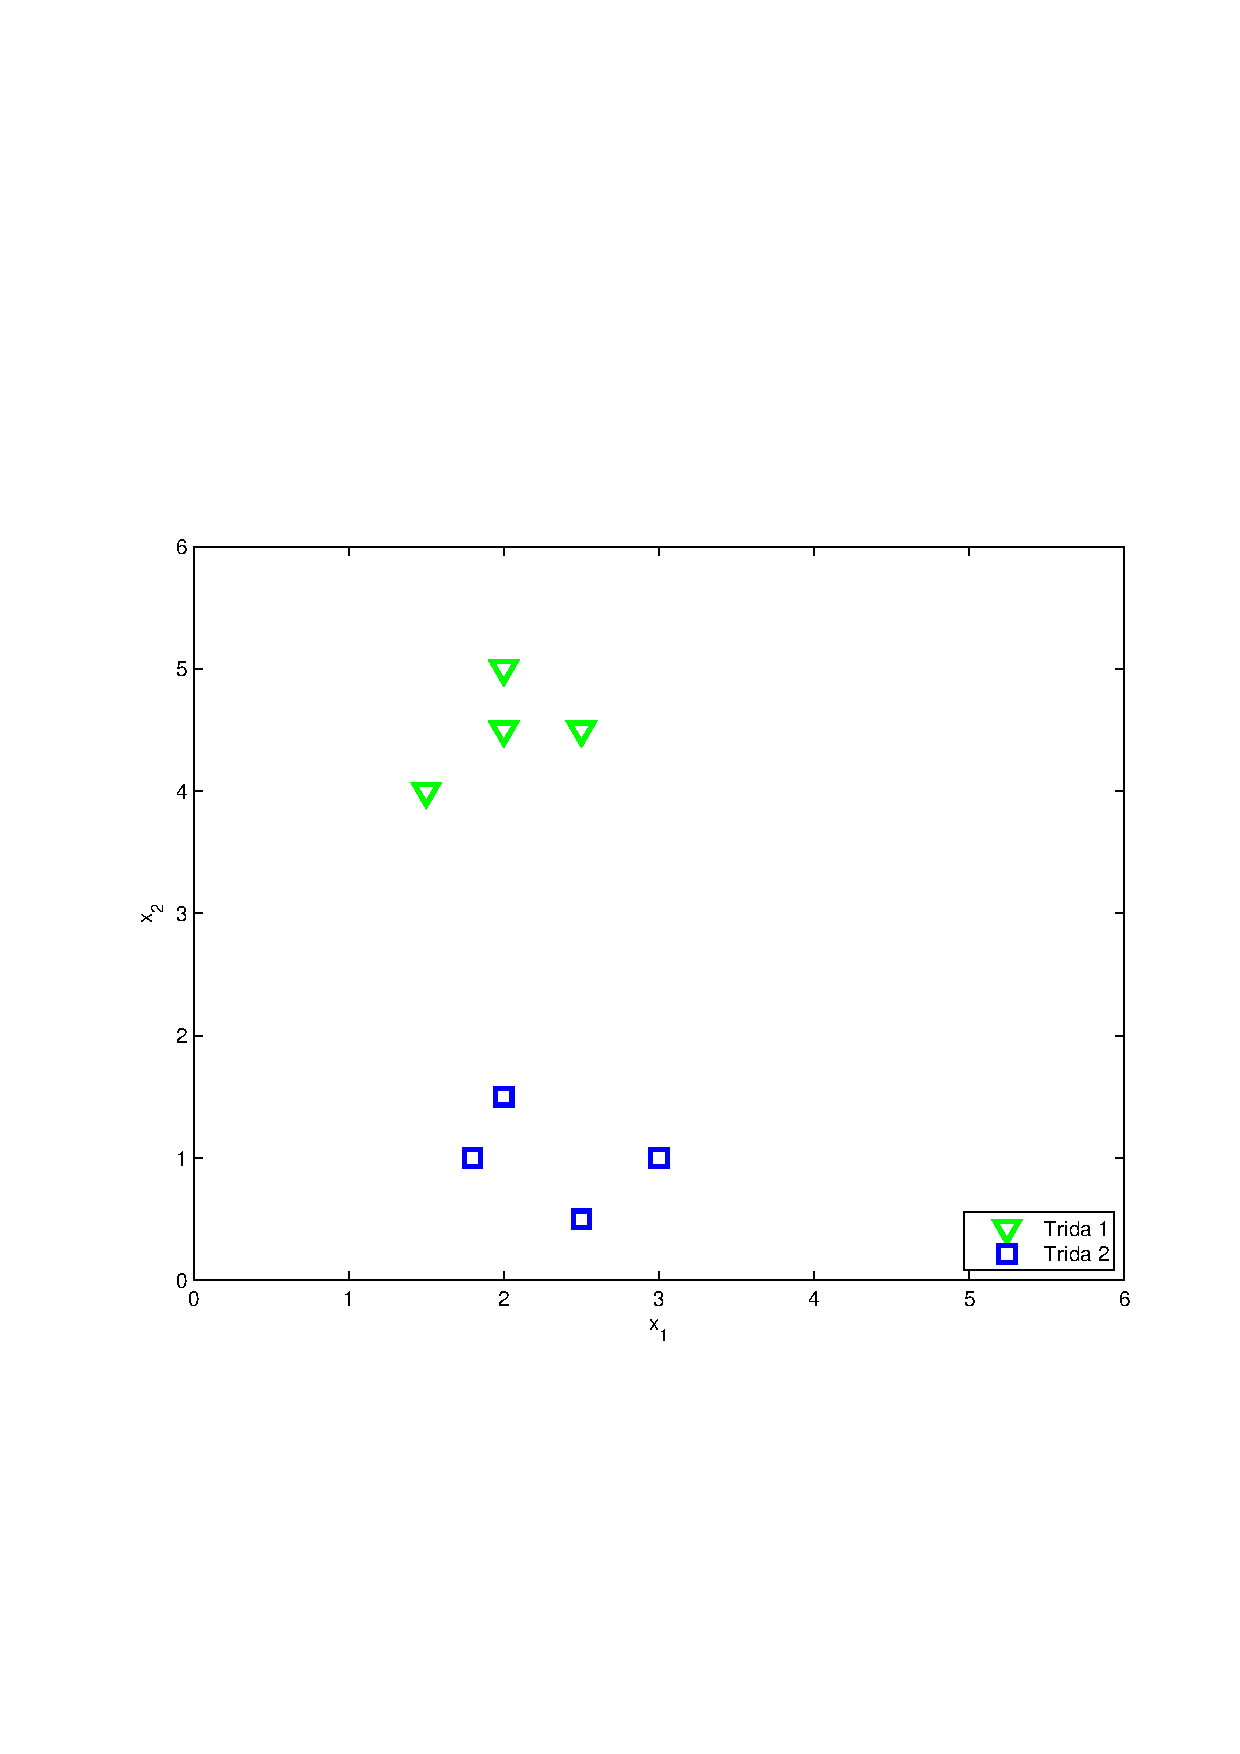
\includegraphics[width = \textwidth, trim = 2.5cm 7cm 2cm 9cm]{./Img/BinarniRegrese/oneVSallClassification/oneVSall_one.pdf}
  		\caption{Klasifikace do dvou tříd.}
		\label{fig:oneVSall_one}
	\end{minipage}%
	\hfill
	\begin{minipage}[b]{0.48\textwidth}
		%trim option's parameter order: left bottom right top
		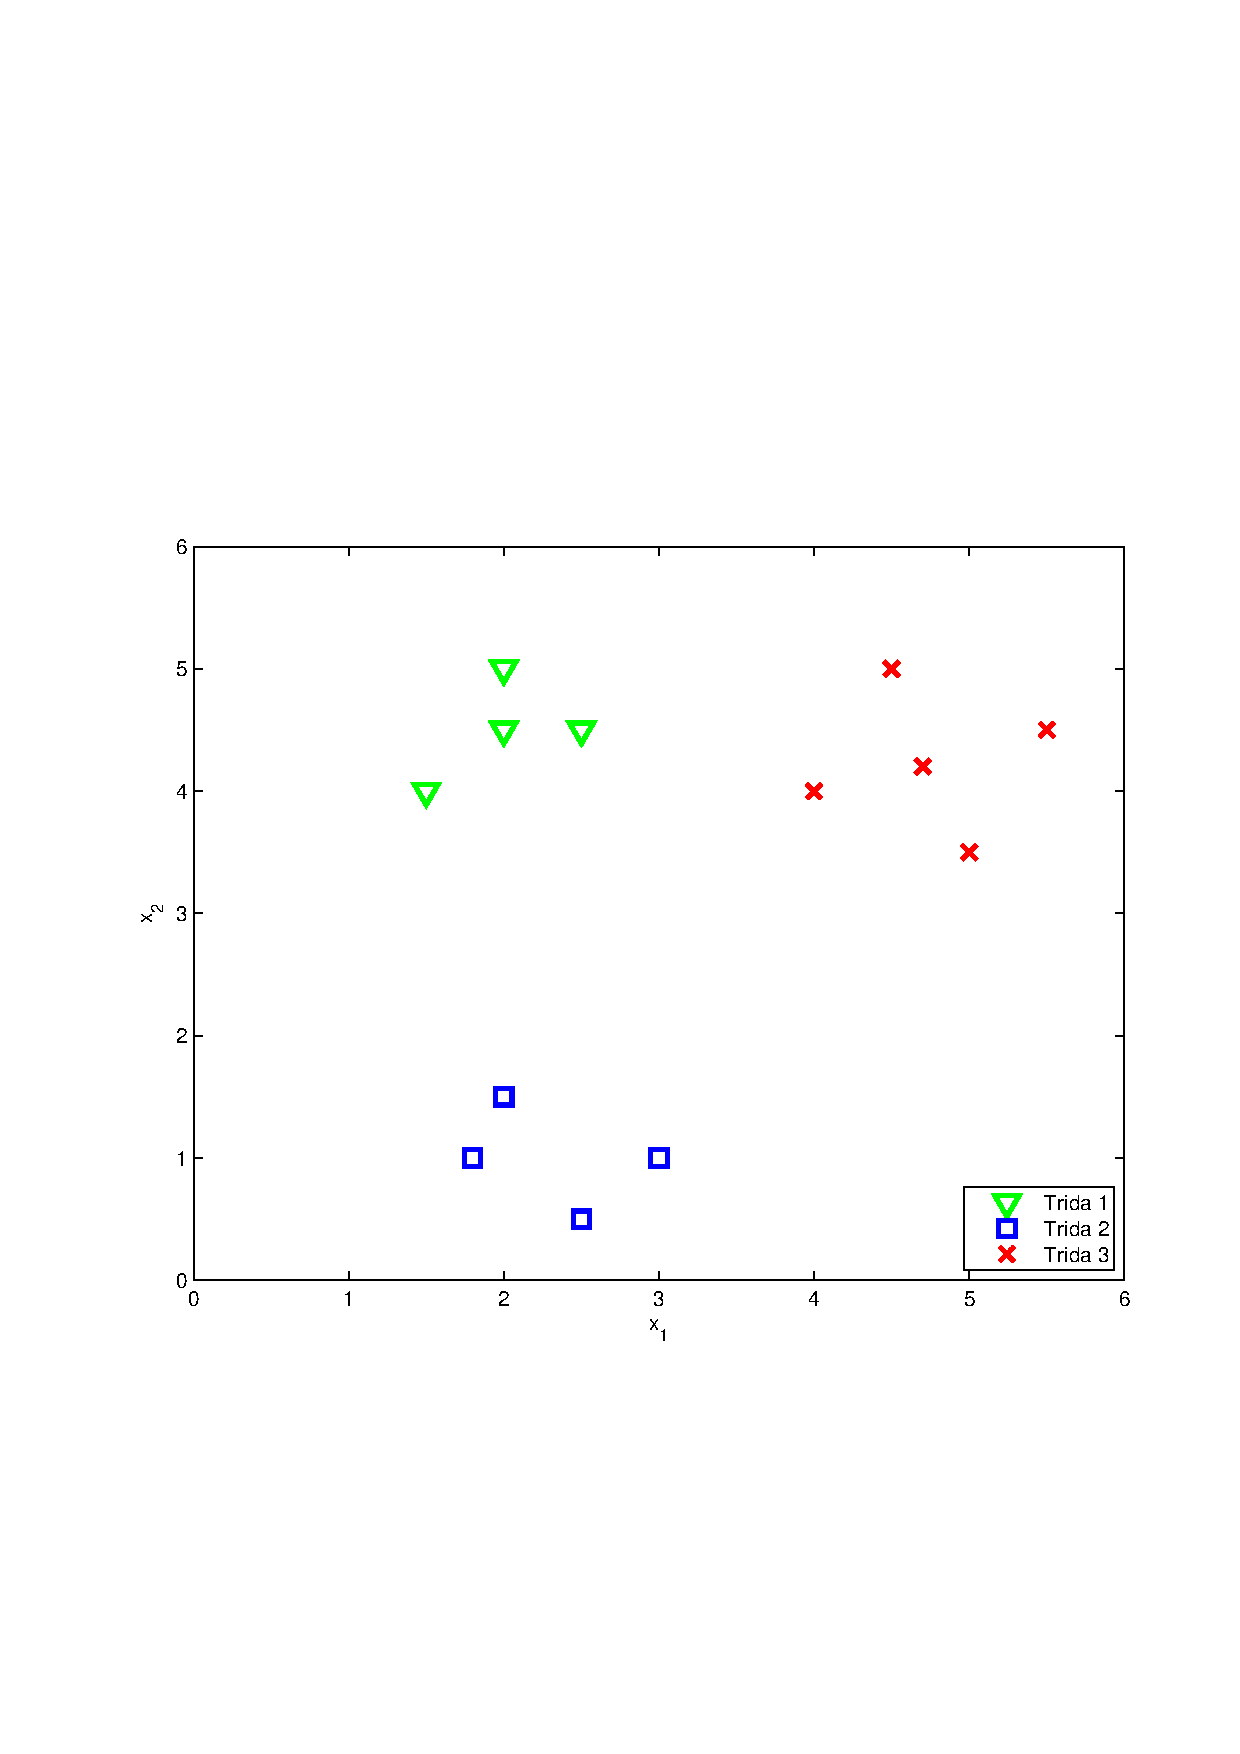
\includegraphics[width = \textwidth, trim = 2.5cm 7cm 2cm 9cm]{./Img/BinarniRegrese/oneVSallClassification/oneVSall_all.pdf}
  		\caption{Klasifikace do více tříd.}
		\label{fig:oneVSall_all}
	\end{minipage}%
\end{figure}}

\par{Z předešlých sekcí víme jak klasifikovat do dvou tříd. Nyní tento přístup použijeme při řešení problému klasifikace do více tříd. Na Obr. \ref{fig:oneVSall_all2} je znázorněno rozložení tříd a~následně na Obr.~\ref{fig:oneVSall_1} je ukázána klasifikace třídy~1 proti třídě, která je zkonstruována spojením všech ostatních tříd (v~našem případě tříd 2~a~3). Na dalších Obr.~\ref{fig:oneVSall_2} a~\ref{fig:oneVSall_3} jsou naznačeny zbylé kombinace.}Pro jednotlivé klasifikace je nutné vytvořit hypotézu
\begin{equation}
	h_{\bm{\Theta}}^{\left( i \right)} \left( \bm{x} \right), \quad i \in \{ 1,~2,~3\},
\end{equation}
která odpovídá pravděpodobnostem
\begin{equation}
	h_{\bm{\Theta}}^{\left( i \right)} \left( \bm{x} \right) = P \left( y = i| \bm{x} ; \bm{\Theta} \right).
\end{equation}}
\pagebreak

\begin{figure}[!ht]
	\centering
	\begin{minipage}[b]{0.48\textwidth}
  		%trim option's parameter order: left bottom right top
		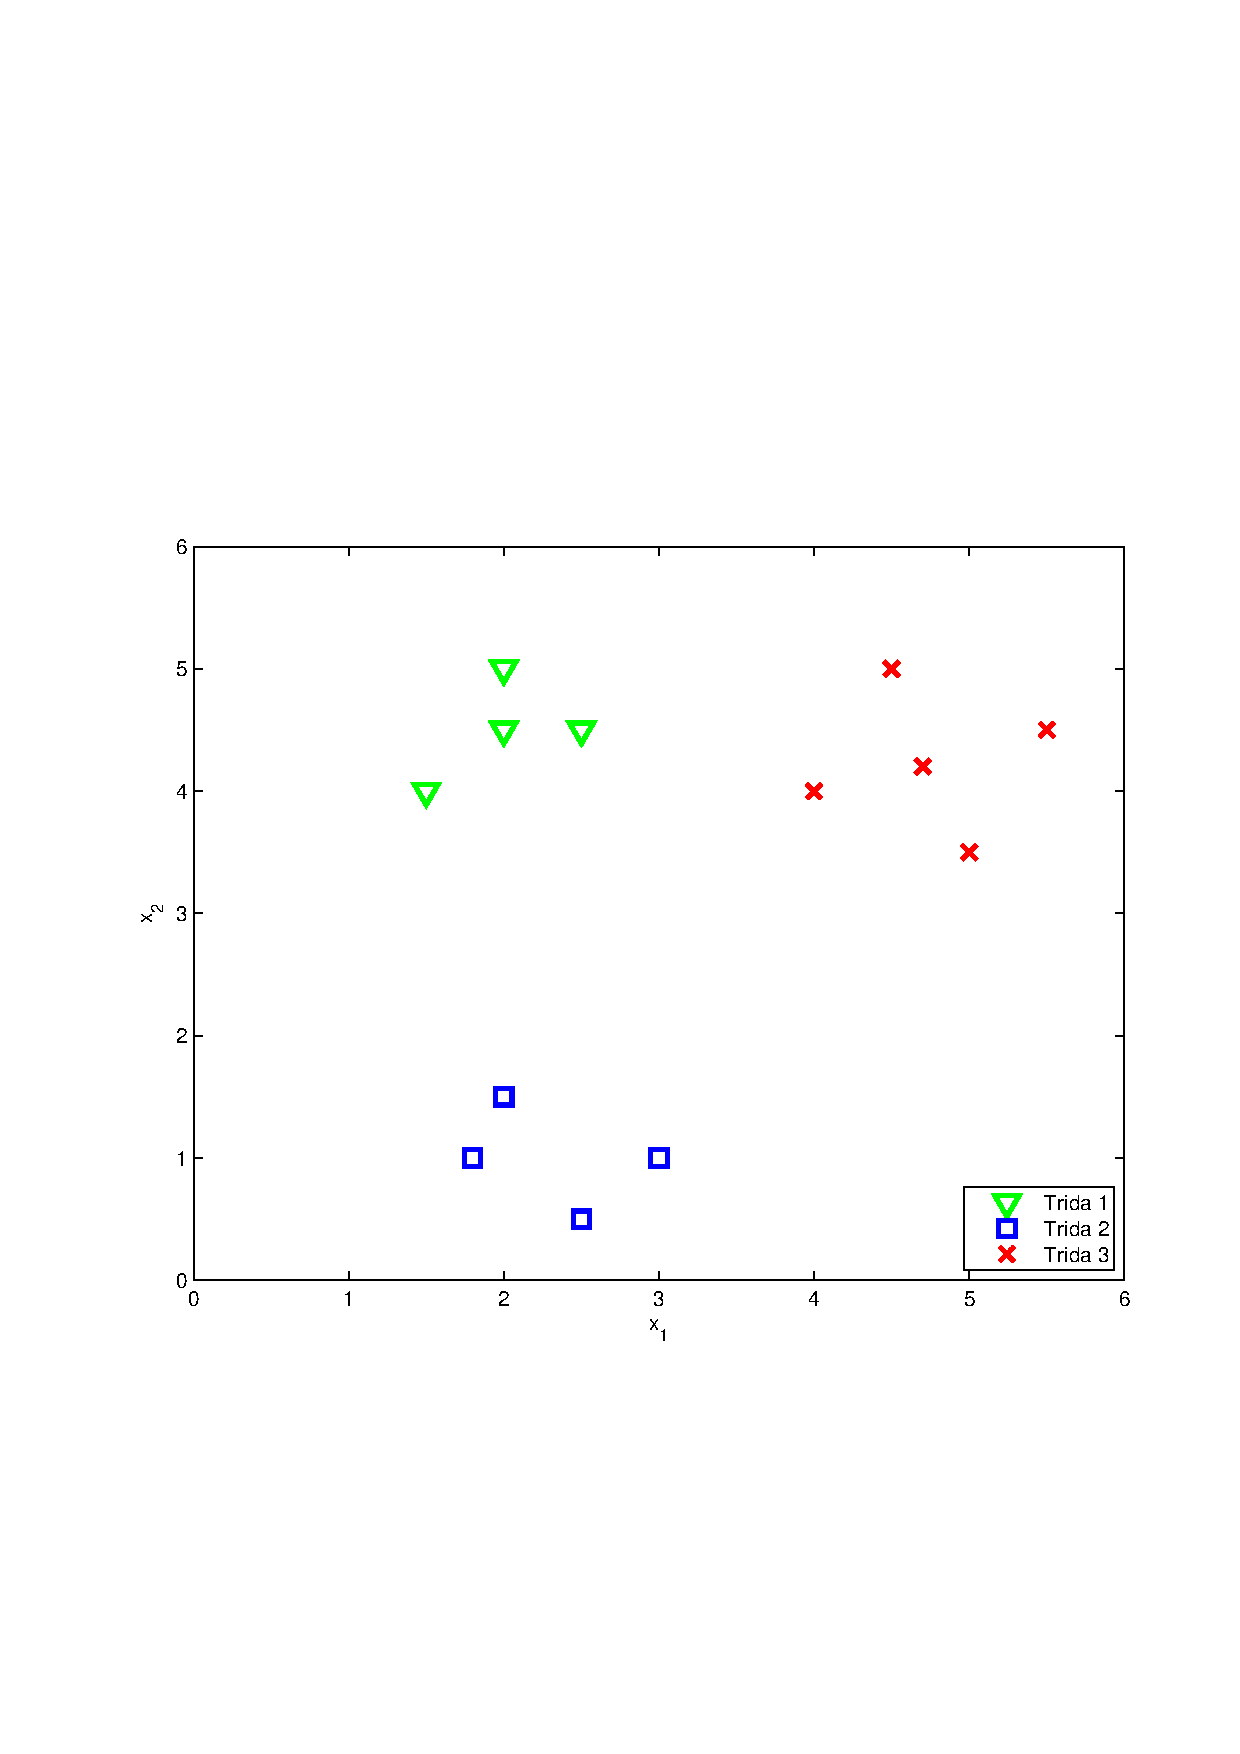
\includegraphics[width = \textwidth, trim = 2.5cm 7cm 2cm 9cm]{./Img/BinarniRegrese/oneVSallClassification/oneVSall_all.pdf}
  		\caption{Rozložení tříd $y = \{1,~2,~3\}$.}
		\label{fig:oneVSall_all2}
	\end{minipage}%
	\hfill
	\begin{minipage}[b]{0.48\textwidth}
		%trim option's parameter order: left bottom right top
		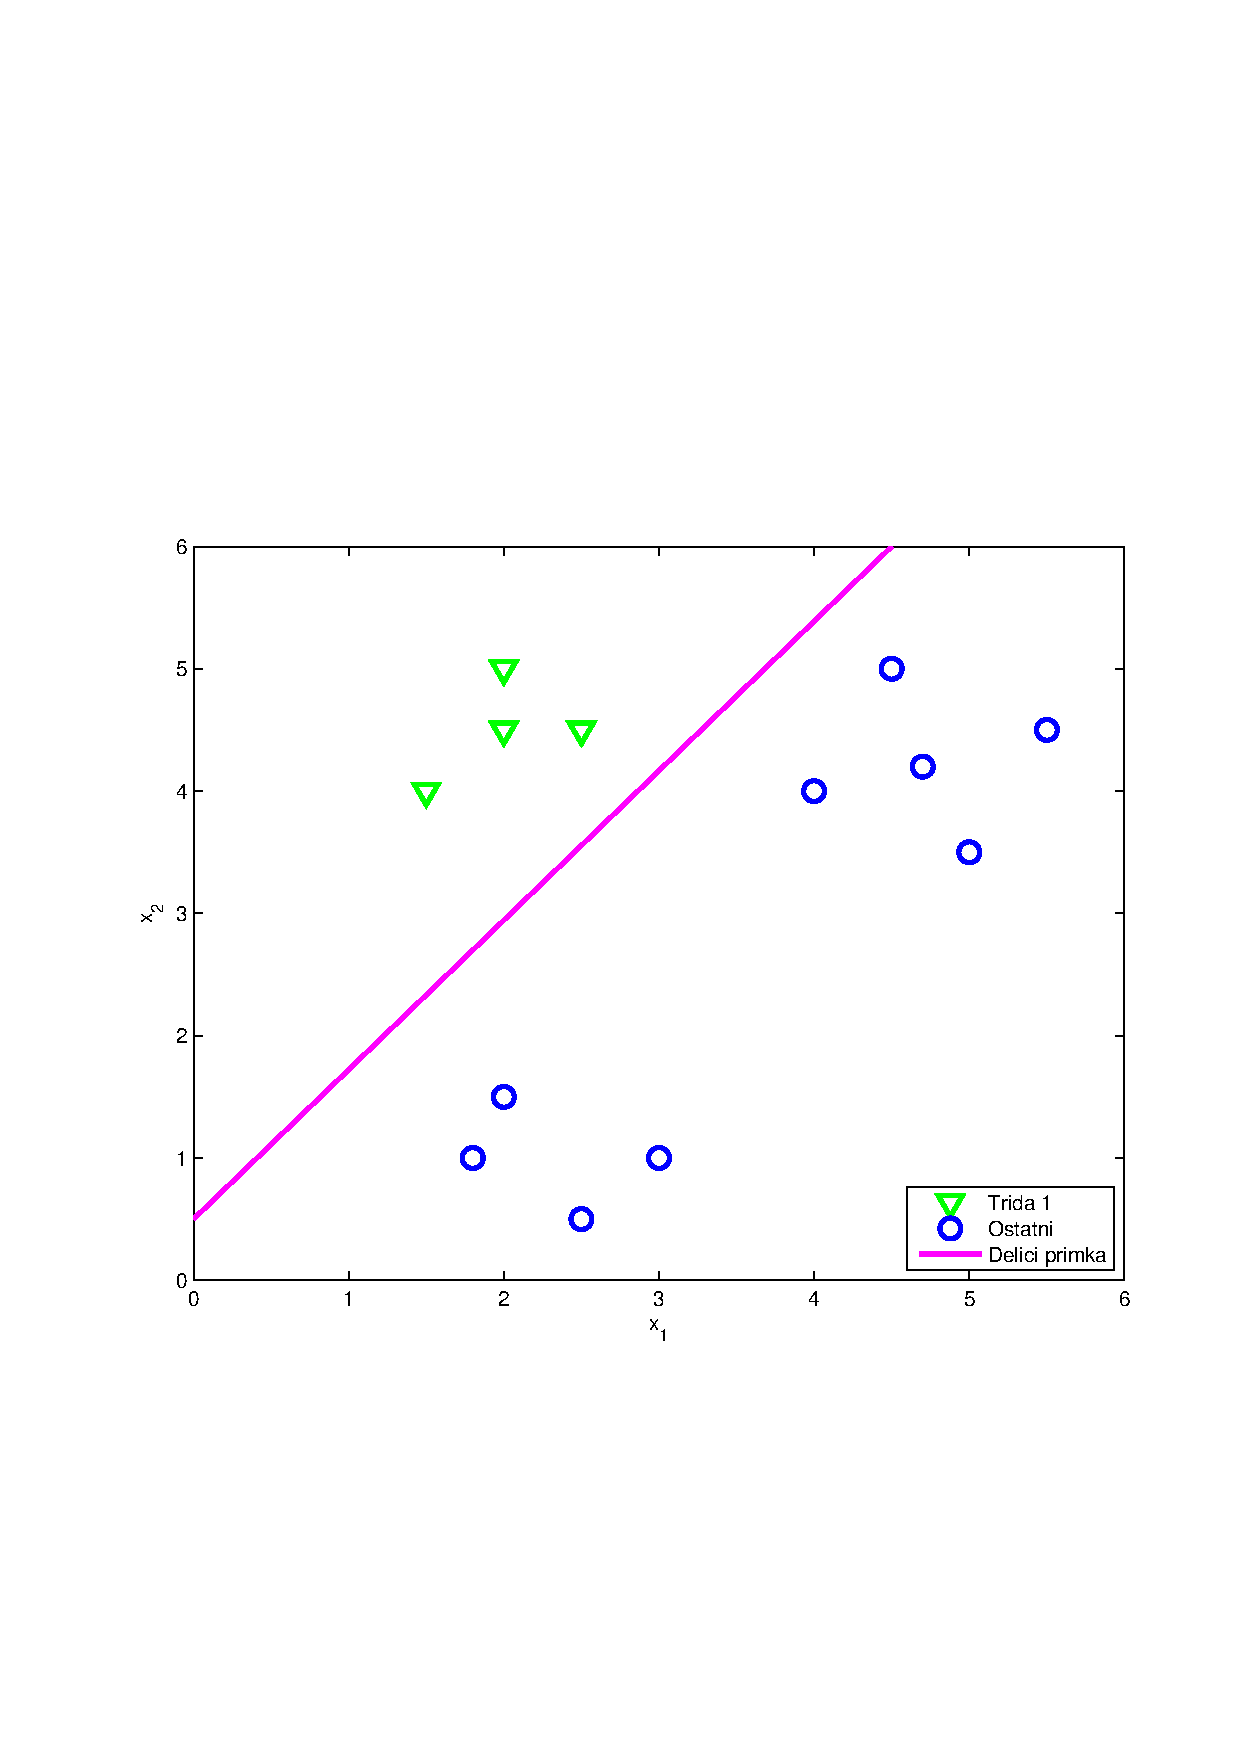
\includegraphics[width = \textwidth, trim = 2.5cm 7cm 2cm 9cm]{./Img/BinarniRegrese/oneVSallClassification/oneVSall_1.pdf}
  		\caption{Klasifikace třídy 1.}
		\label{fig:oneVSall_1}
	\end{minipage}%
\end{figure}
\begin{figure}[!ht]
	\centering
	\begin{minipage}[b]{0.48\textwidth}
  		%trim option's parameter order: left bottom right top
		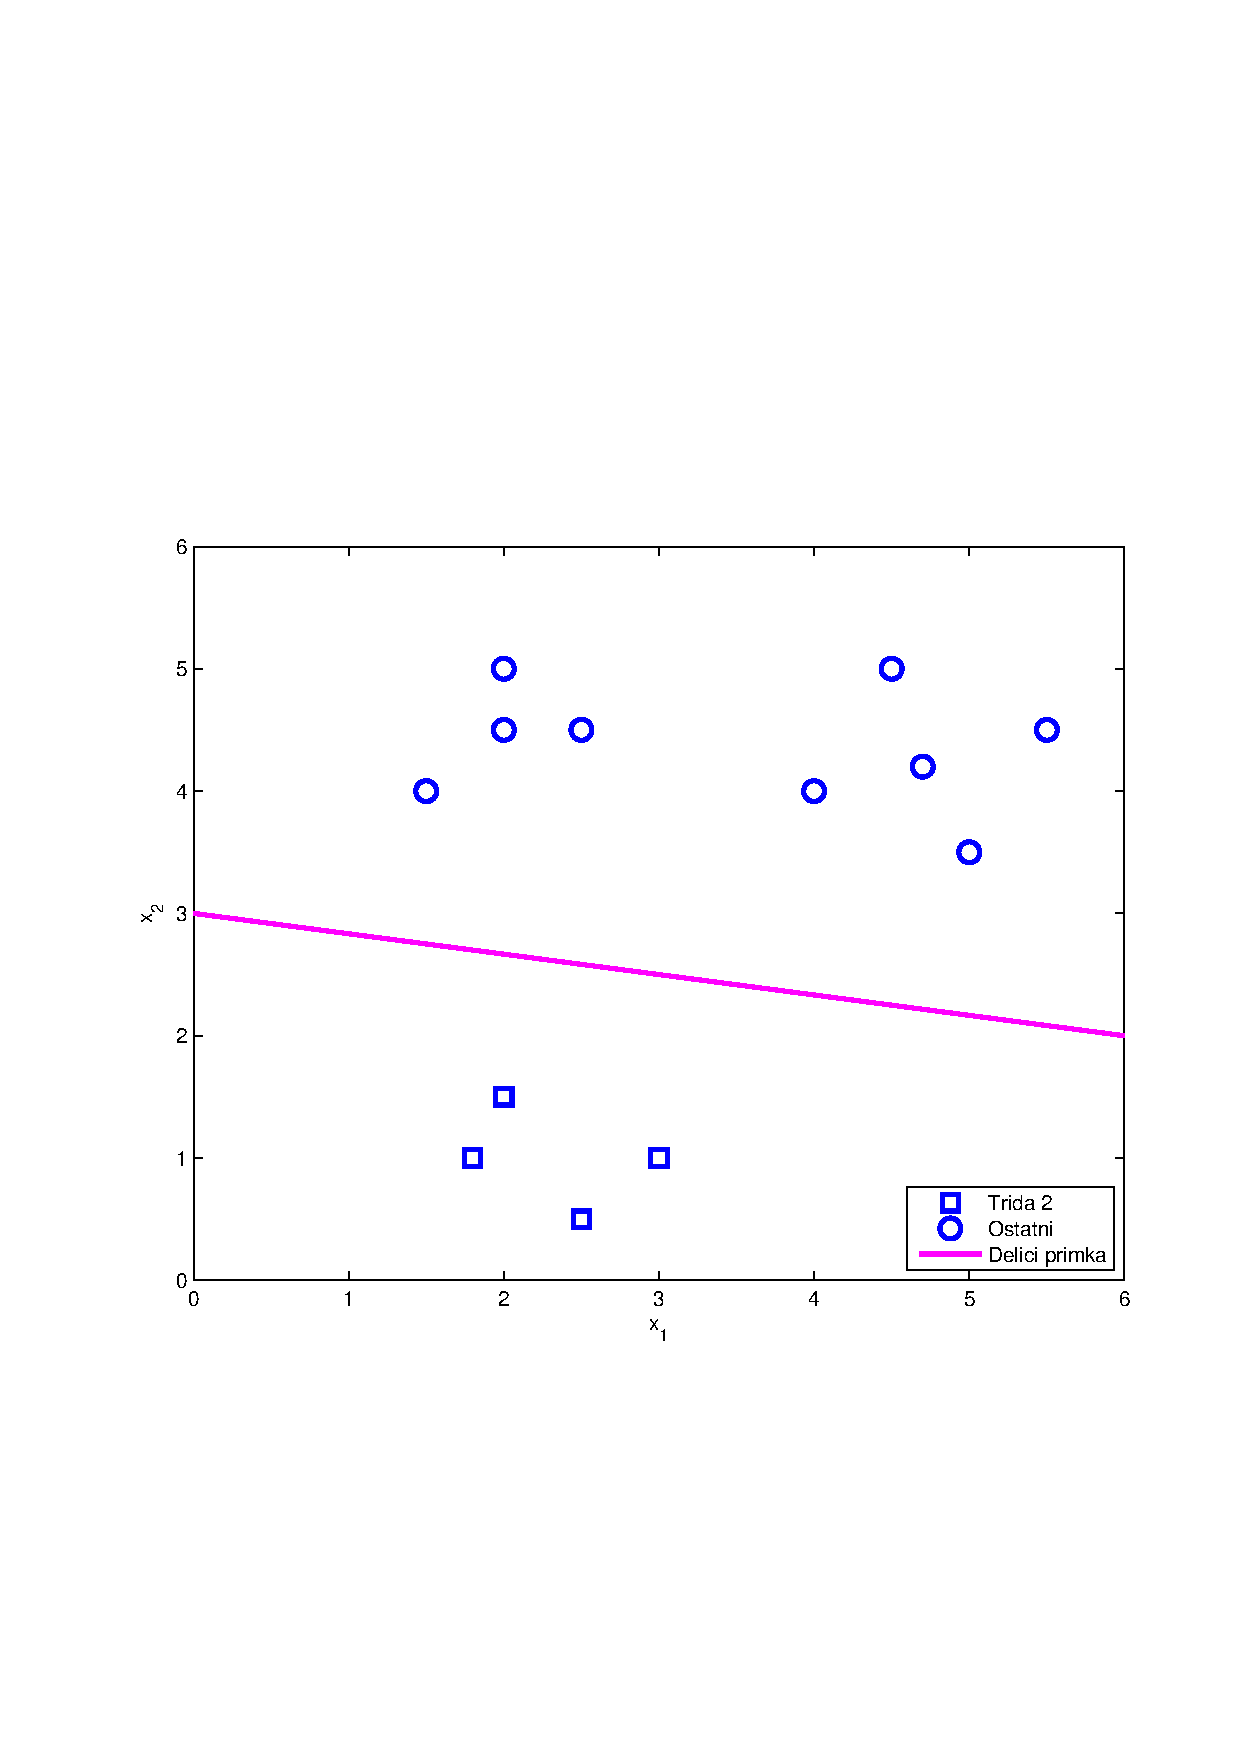
\includegraphics[width = \textwidth, trim = 2.5cm 7cm 2cm 9cm]{./Img/BinarniRegrese/oneVSallClassification/oneVSall_2.pdf}
  		\caption{Klasifikace třídy 2.}
		\label{fig:oneVSall_2}
	\end{minipage}%
	\hfill
	\begin{minipage}[b]{0.48\textwidth}
		%trim option's parameter order: left bottom right top
		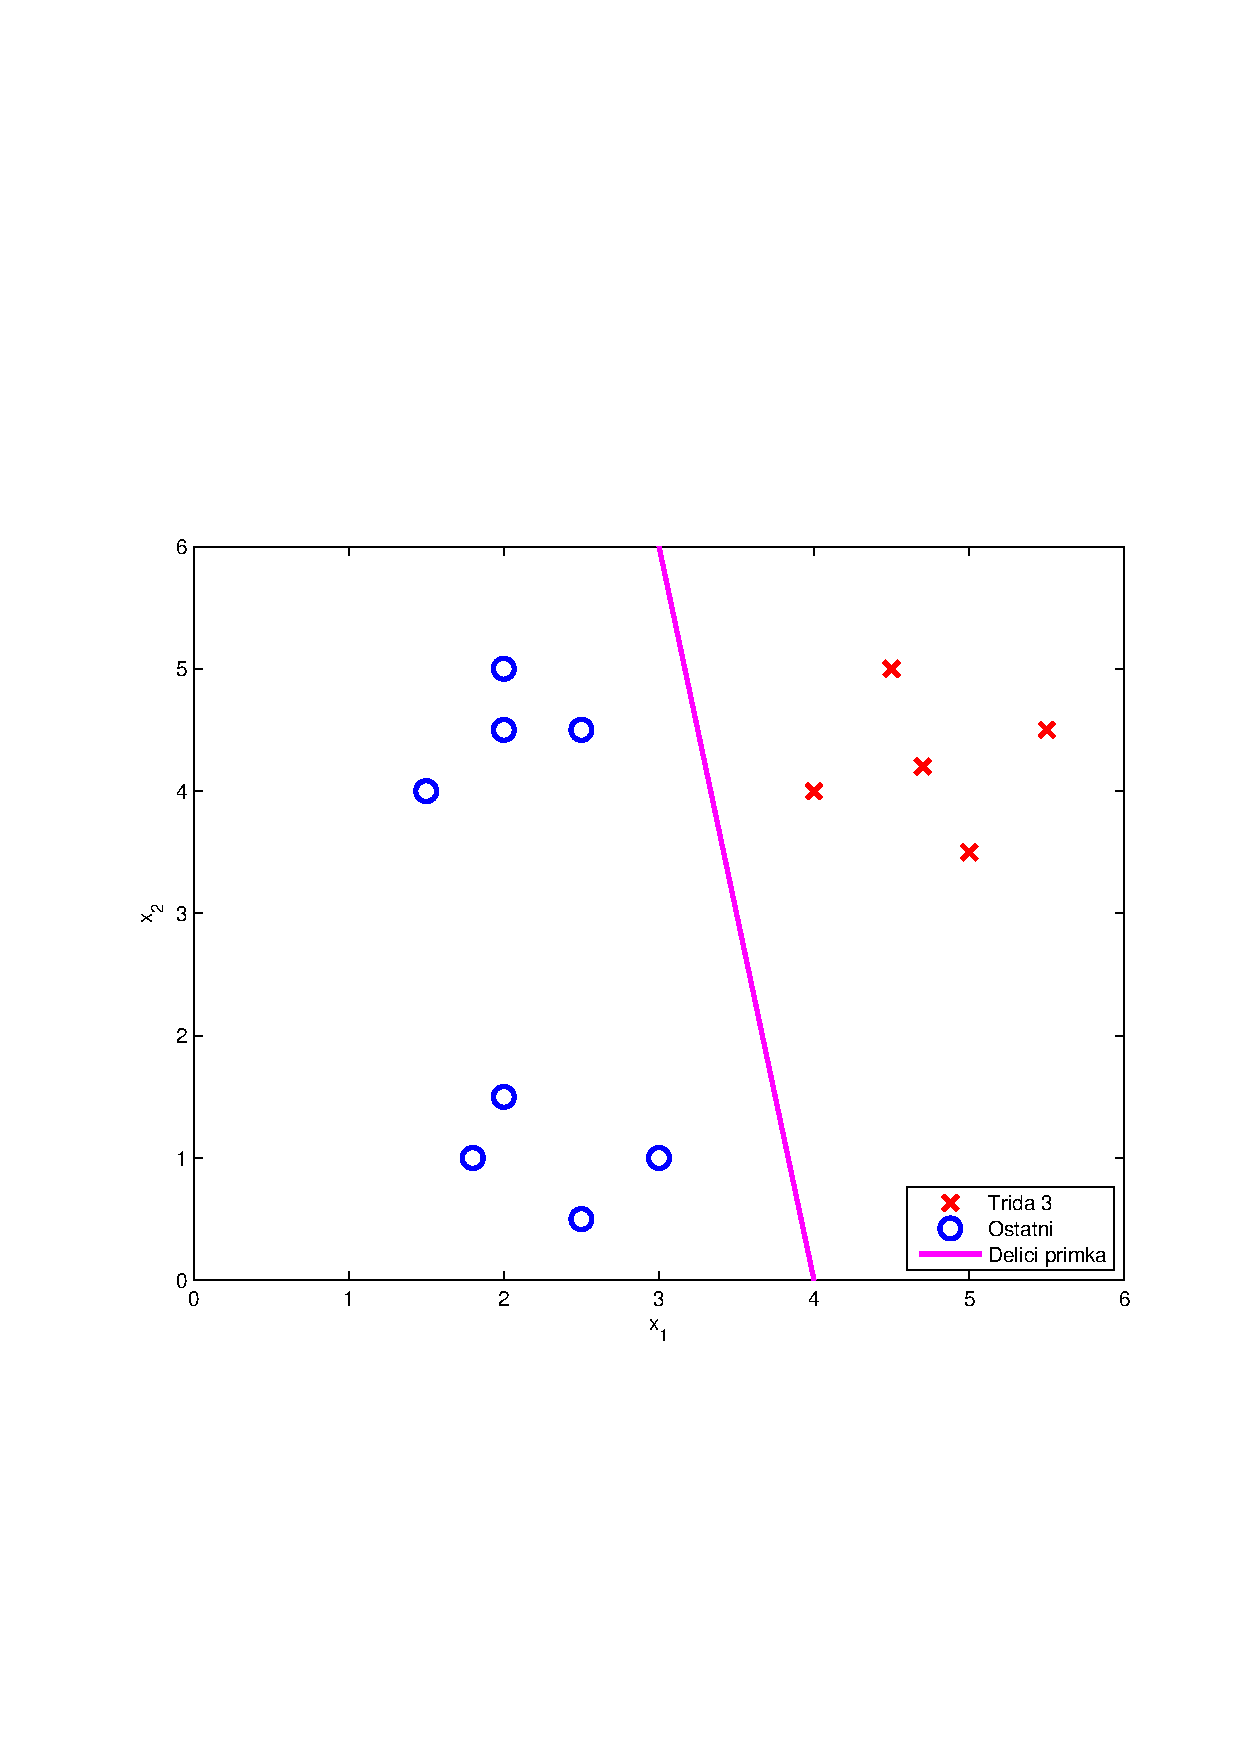
\includegraphics[width = \textwidth, trim = 2.5cm 7cm 2cm 9cm]{./Img/BinarniRegrese/oneVSallClassification/oneVSall_3.pdf}
  		\caption{Klasifikace třídy 3.}
		\label{fig:oneVSall_3}
	\end{minipage}%
\end{figure}

\subsubsection*{Shrnutí}
\par{Nejdříve je nutné natrénovat binární klasifikátory $h_{\bm{\Theta}}^{\left( i \right)} \left( \bm{x} \right)$ pro všechny třídy $i$ pro predikci pravděpodobnosti, že vzorek bude patřit do třídy $y = i$. Následně pro nový vstup $x$ klasifikovat podle všech hypotéz a vybrat takovou třídu $i$, která maximalizuje pravděpodobnost hypotézy
\begin{equation}
	 \max_{i} h_{\bm{\Theta}}^{\left( i \right)} \left( \bm{x} \right).
\end{equation}}


\newpage
































%----REGULARIZACE------------------------------------------------------------------------------------
\section{Regularizace}
\label{sec:Regularizace}
















%----PROBLEM-PRETRENOVANI---------------------------------------------------------------------------
\subsection{Problém přetrénování}
\label{sec:RegularizaceProblemPretrenovani}

\par{Nyní když známe algoritmy lineární a binární regrese, které se hodí pro řešení mnoha úloh strojového učení, musíme si říci něco o problému zvaném přetrénování. Tento problém způsobuje, že dané algoritmy ve výsledku fungují velmi špatně.}

\par{V této sekci si vysvětlíme v čem problém přetrénování spočívá a v následujících sekcích bude popsán postup jak se s daným problémem vypořádat.}

\par{Vraťme se k našemu problému predikce ceny velikosti bytu, ve kterém jsme využili algoritmu lineární regrese.}

\par{Na Obr.~\ref{fig:regrese_0} jsou znázorněná trénovací data. Pokud využijeme lineární regresi společně s hypotézou $h_{\bm{\Theta}} \left( \bm{x} \right) = \vartheta_0 + \vartheta_1 x$, tak získáme predikci ve tvaru, který lze vidět na Obr. \ref{fig:regrese_1}. V tomto případě naše zvolená hypotéza $h_{\bm{\Theta}} \left( \bm{x} \right)$ nerespektuje dostatečně tvar našich trénovacích dat. Přesnější anglický termín pro takto nastalou situaci zní \textit{underfit} nebo \textit{high bias}, což se dá vysvětlit jako problém, kdy se snažíme použít regresi na trénovací data s~málo komplexní hypotézou. Tedy hypotéza nemůže dostatečně přesně vystihovat tvar dat (nezobecňuje).}
\begin{figure}[!ht]
	\centering
	\begin{minipage}[t]{0.48\textwidth}
  		%trim option's parameter order: left bottom right top
		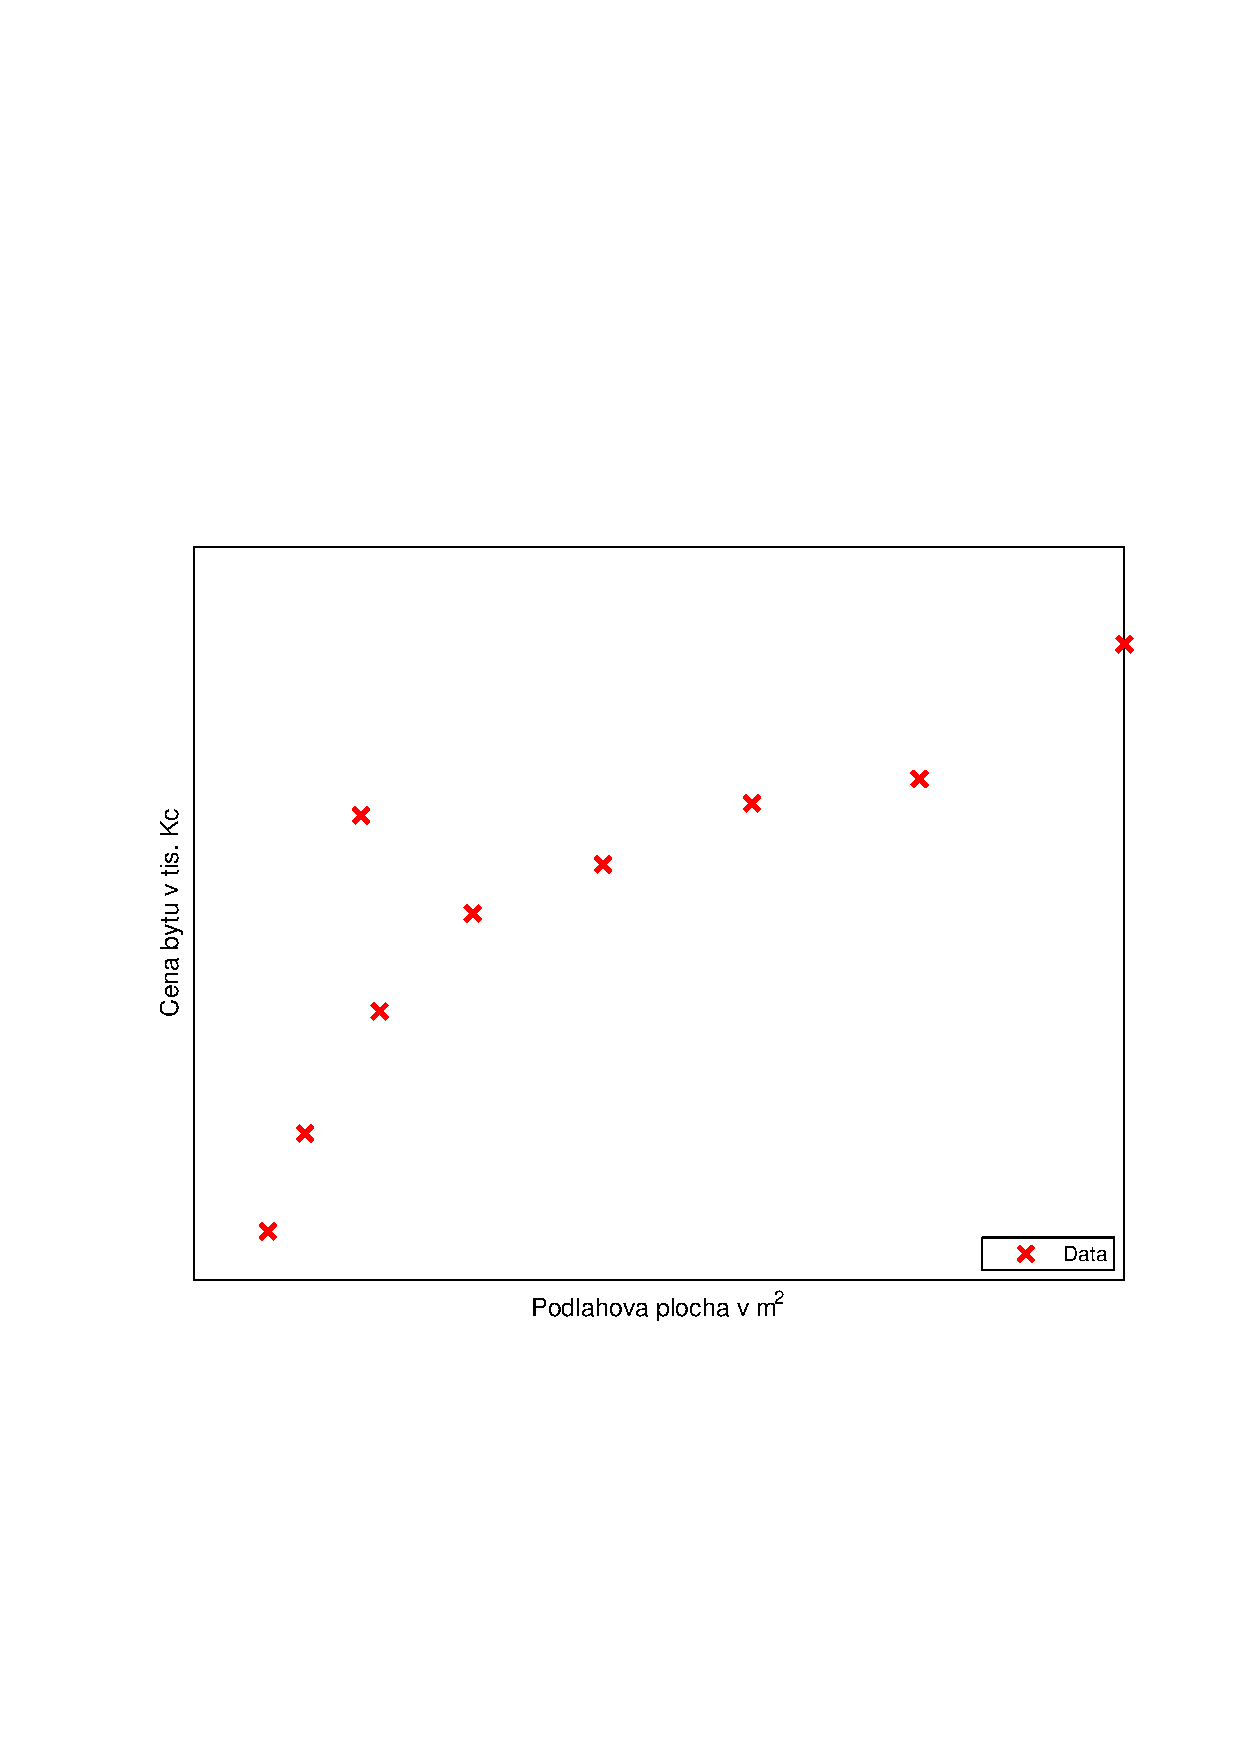
\includegraphics[width = \textwidth, trim = 2.5cm 7cm 2cm 9cm]{./Img/Regularizace/Pretrenovani1D/regrese_0.pdf}
  		\caption{Trénovací data.}
		\label{fig:regrese_0}
	\end{minipage}%
	\hfill
	\begin{minipage}[t]{0.48\textwidth}
		%trim option's parameter order: left bottom right top
		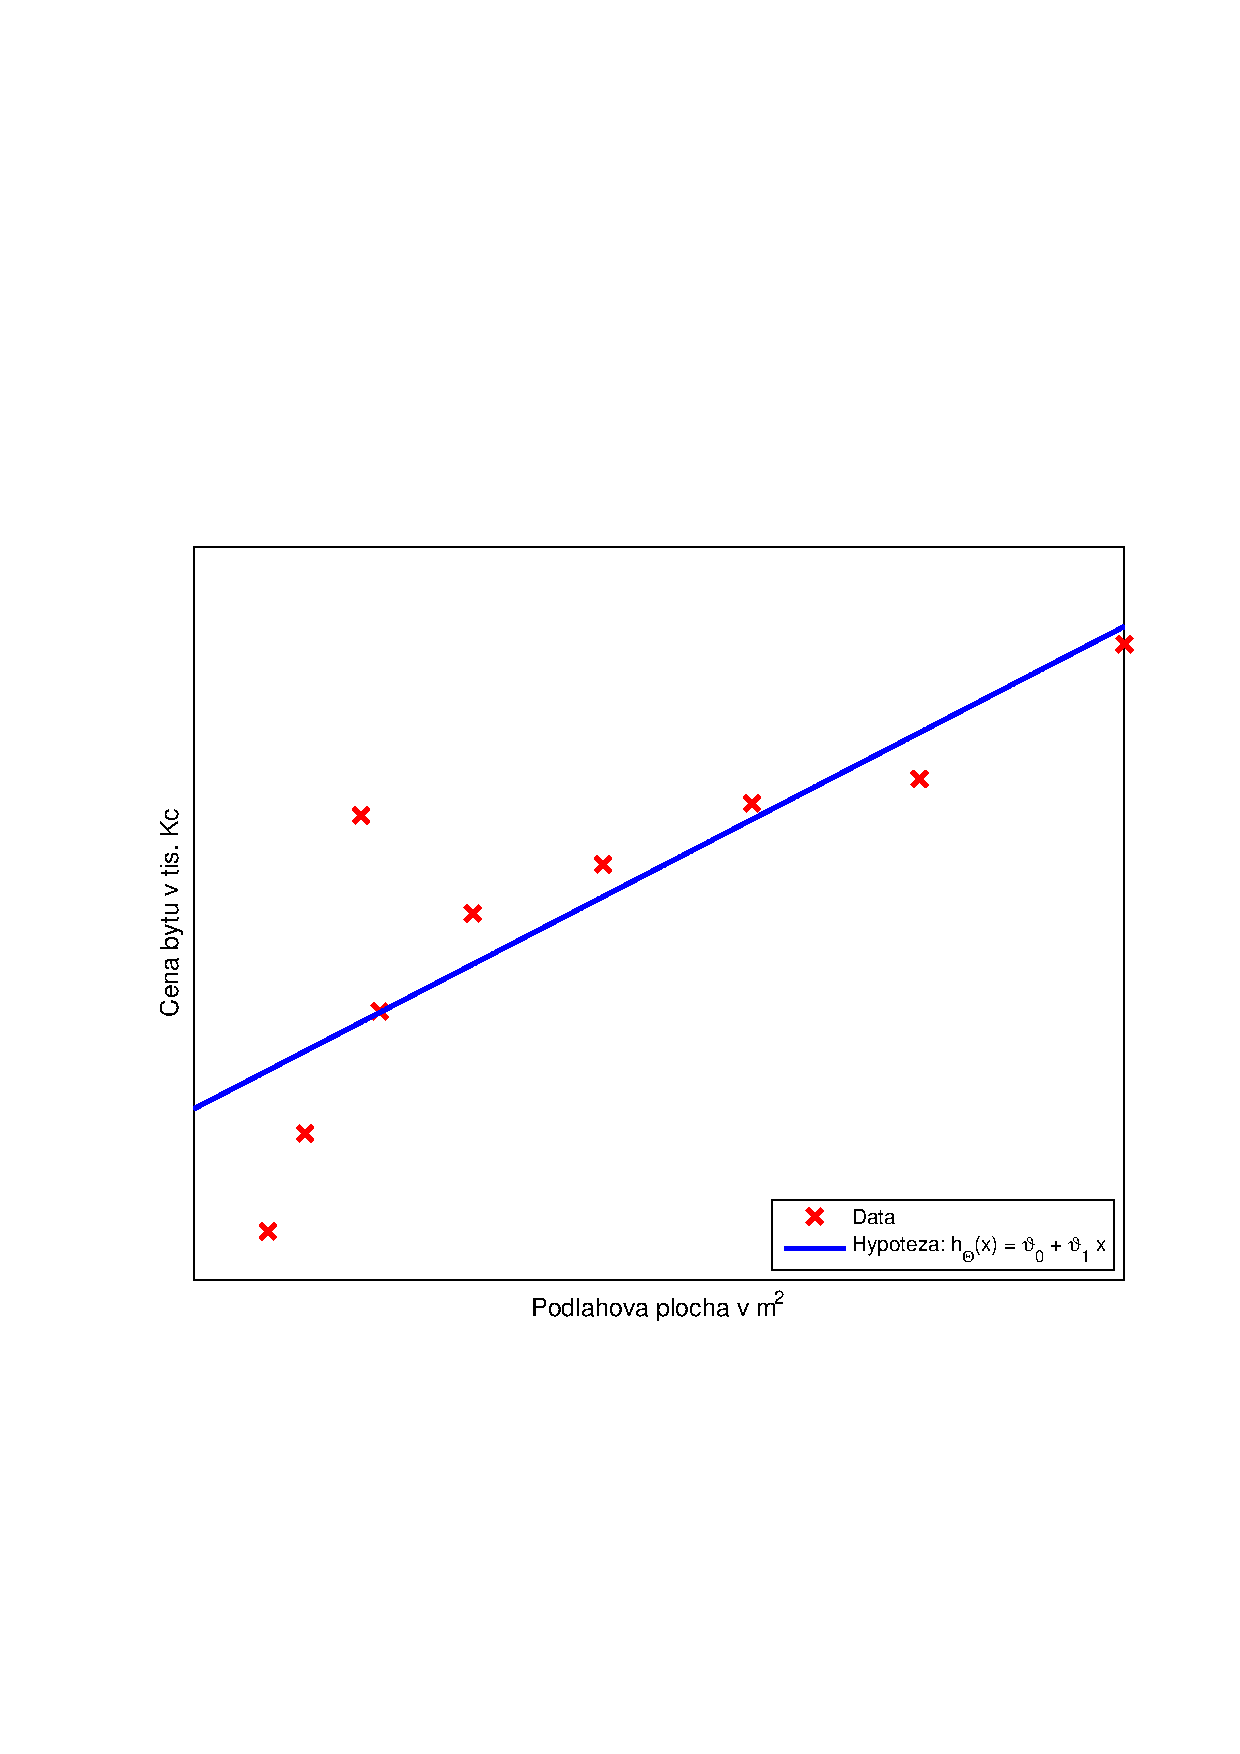
\includegraphics[width = \textwidth, trim = 2.5cm 7cm 2cm 9cm]{./Img/Regularizace/Pretrenovani1D/regrese_1.pdf}
  		\caption{Lineární regrese (\textit{underfit}, \textit{high bias}).}	
		\label{fig:regrese_1}
	\end{minipage}%
\end{figure}
\pagebreak

\par{Na Obr. \ref{fig:regrese_2} lze vidět regresi s hypotézou ve tvaru $h_{\bm{\Theta}} \left( \bm{x} \right) = \vartheta_0 + \vartheta_1 x + \vartheta_2 x^2$, která velmi dobře zobecňuje trénovací data a proto by byla v tomto případě nejlepší volbou.}

\par{Dále na Obr. \ref{fig:regrese_4} lze vidět regresi s hypotézou $h_{\bm{\Theta}} \left( \bm{x} \right) = \vartheta_0 + \vartheta_1 x + \vartheta_2 x^2 + \vartheta_2 x^3 + \vartheta_2 x^4$, jejíž chování je velmi \uv{divoké} a nezobecňuje trénovací data. V tomto případě se snaží hypotéza co nejvíce respektovat trénovací data za cenu ztráty obecnosti. Tento problém se nazývá přetrénování, anglicky \textit{overfitting} nebo \textit{high variance}.}

\begin{figure}[!ht]
	\centering
	\begin{minipage}[t]{0.48\textwidth}
  		%trim option's parameter order: left bottom right top
		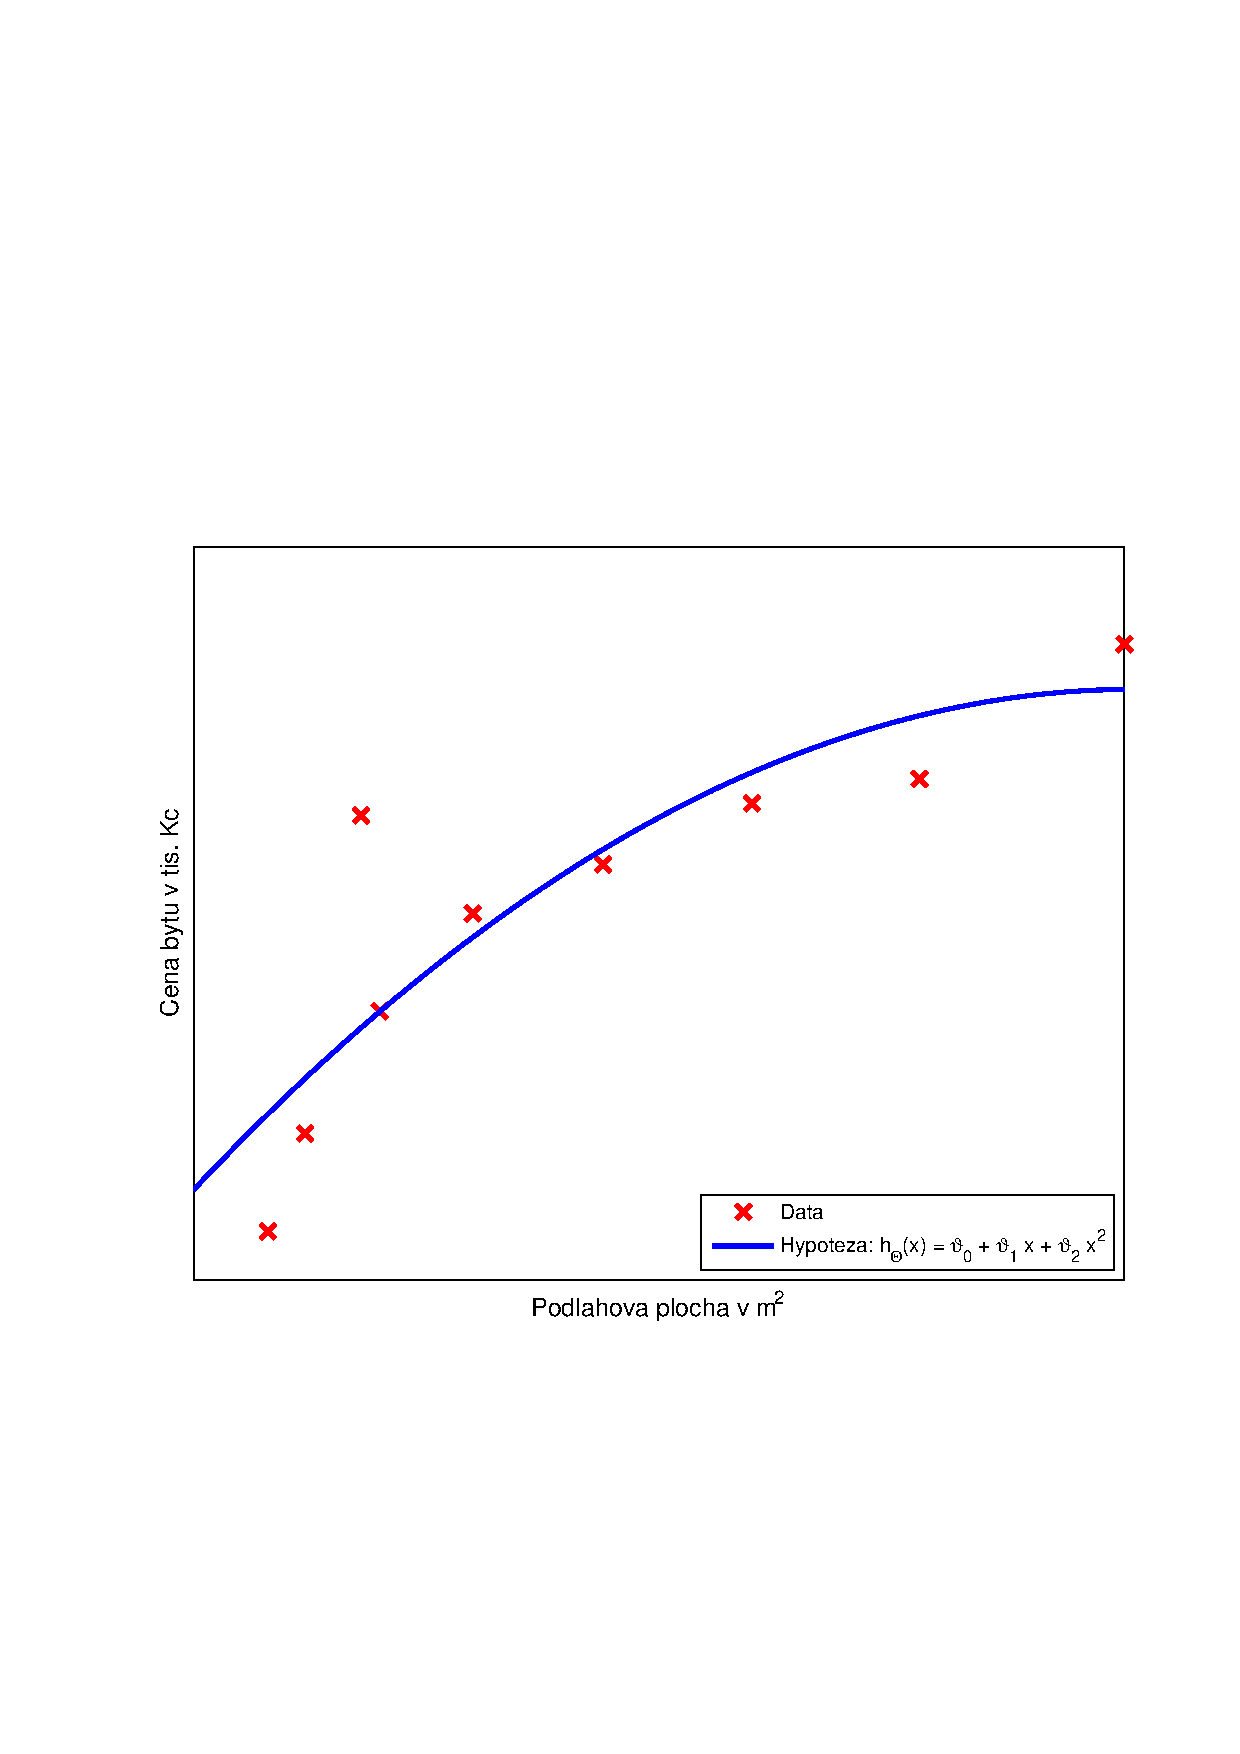
\includegraphics[width = \textwidth, trim = 2.5cm 7cm 2cm 9cm]{./Img/Regularizace/Pretrenovani1D/regrese_2.pdf}
  		\caption{Regrese pomocí hypotézy ve tvaru polynomu druhého stupně (\textit{just right}).}
		\label{fig:regrese_2}
	\end{minipage}%
	\hfill
	\begin{minipage}[t]{0.48\textwidth}
		%trim option's parameter order: left bottom right top
		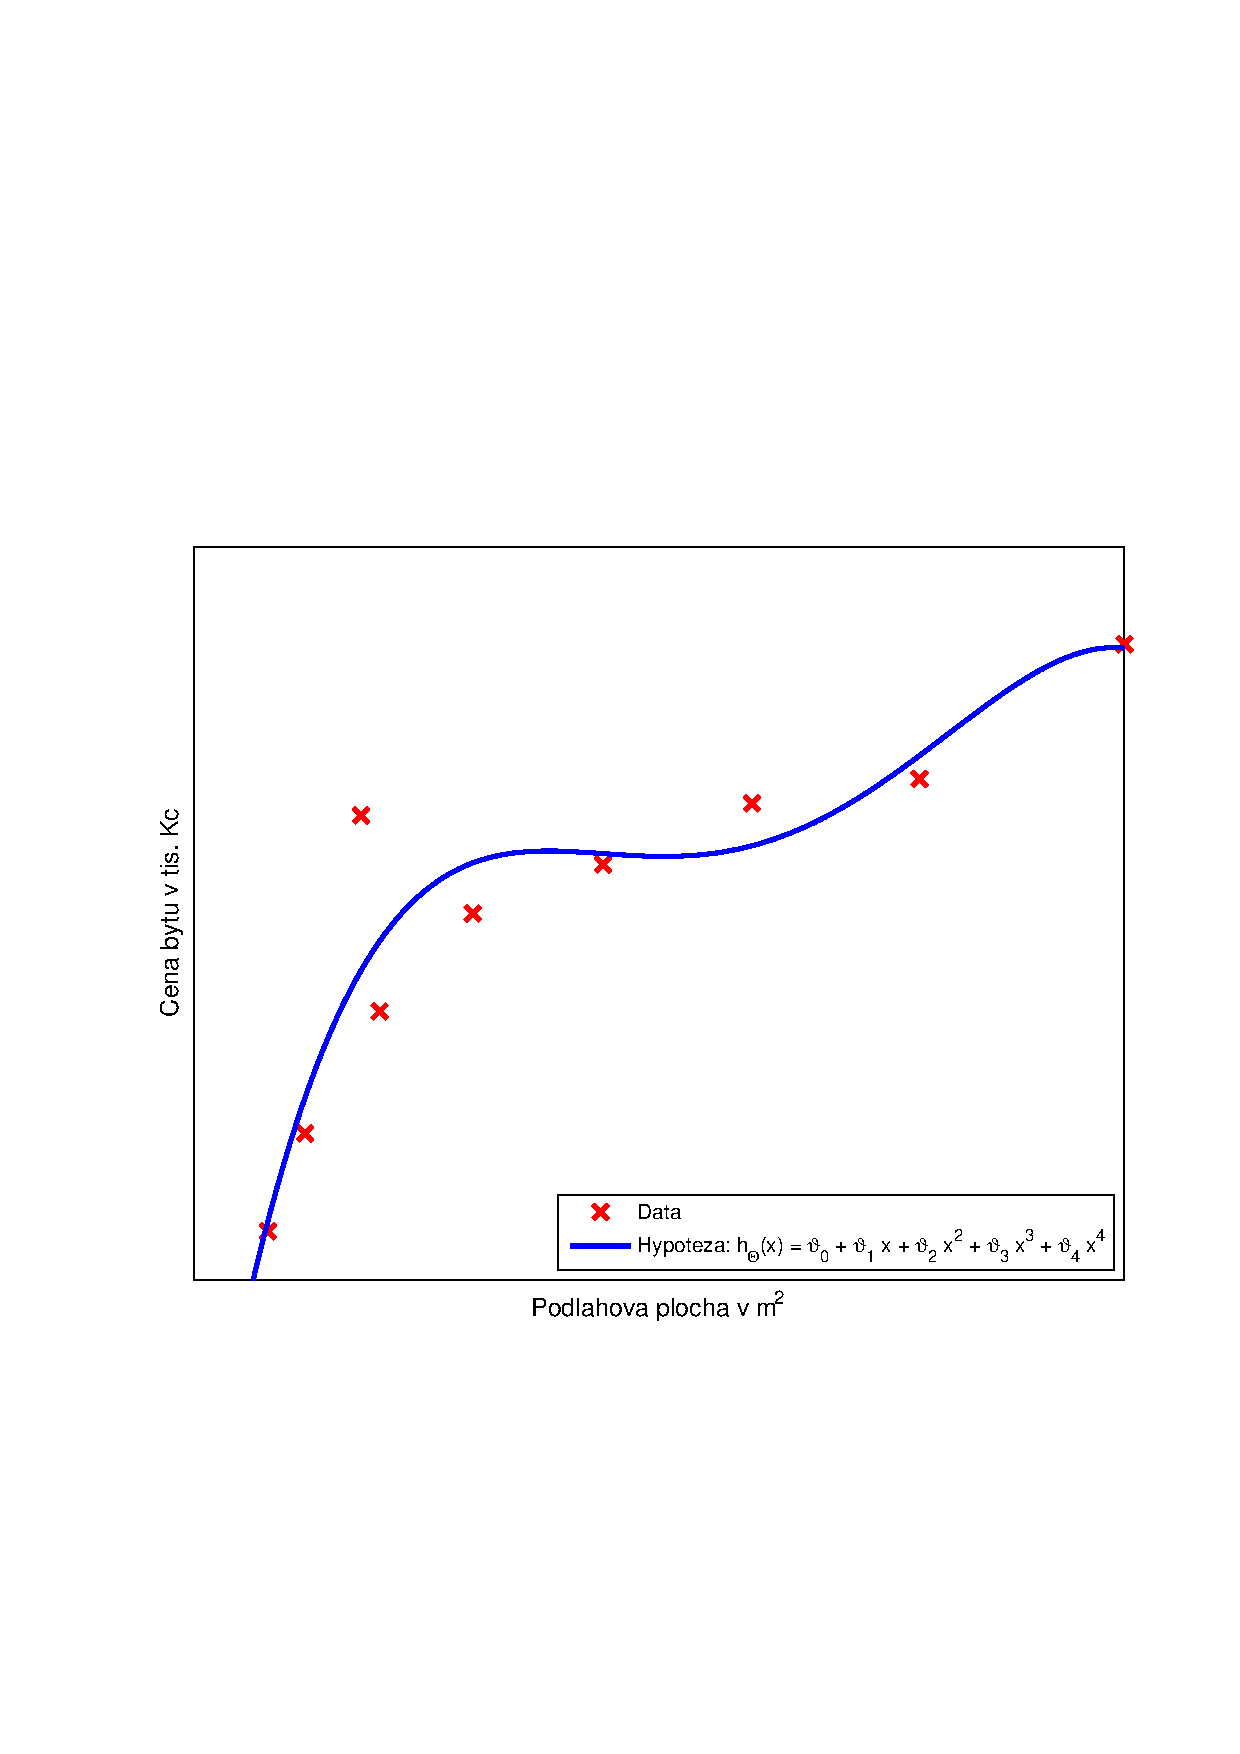
\includegraphics[width = \textwidth, trim = 2.5cm 7cm 2cm 9cm]{./Img/Regularizace/Pretrenovani1D/regrese_4.pdf}
  		\caption{Regrese pomocí hypotézy ve tvaru polynomu čtvrtého stupně (\textit{overfitting}, \textit{high variance}).}
		\label{fig:regrese_4}
	\end{minipage}%
\end{figure}

\subsubsection*{Přetrénování (\textit{overfitting}):}
\par{V případě, že máme příliš mnoho příznaků, hypotéza může velmi dobře respektovat trénovací data $\left( J \left( \bm{\Theta} \right) = \frac{1}{2m} \sum_{i=1}^{m} \left( h_{\bm{\Theta}} \left( \bm{x}^{\left( i \right)} \right) - y^{\left( i \right)} \right)^2 \approx 0 \right)$, ale nebude schopna správně klasifikovat nově příchozí vzorky. Nebude schopna generalizovat, tedy predikce na nově příchozích vzorcích selže.}

\subsubsection*{Možnosti odstranění přetrénování:}
\begin{enumerate}
	\item Redukovat počet příznaků.
		\begin{itemize}
			\item Manuálně zvolit příznaky, které budou zachovány.
			\item Automatická redukce příznaků například PCA.
		\end{itemize}
	\item Regularizace.
		\begin{itemize}
			\item Zachovat všechny příznaky, ale redukovat velikost / váhu parametrů $\vartheta_j$.
			\item Funguje správně pokud máme velké množství příznaků, kde každý malou měrou přispívá k predikci $y$.
		\end{itemize}				
\end{enumerate}



\newpage

















%----ZTRATOVA-FUNKCE-------------------------------------------------------------------------
\subsection{Ztrátová funkce}
\par{V sekci \ref{sec:RegularizaceProblemPretrenovani} jsme si ukázali jak lze pomocí kvadratické hypotézy $h_{\bm{\Theta}} \left( \bm{x} \right) = \vartheta_0 + \vartheta_1 x + \vartheta_2 x^2$ dobře zobecnit naše trénovací data. Dále již víme, že hypotéza ve tvaru $h_{\bm{\Theta}} \left( \bm{x} \right) = \vartheta_0 + \vartheta_1 x + \vartheta_2 x^2 + \vartheta_2 x^3 + \vartheta_2 x^4$ nezobecňuje naší trénovací množinu dat dobře.}
\begin{figure}[!ht]
	\centering
	\begin{minipage}[t]{0.48\textwidth}
  		%trim option's parameter order: left bottom right top
		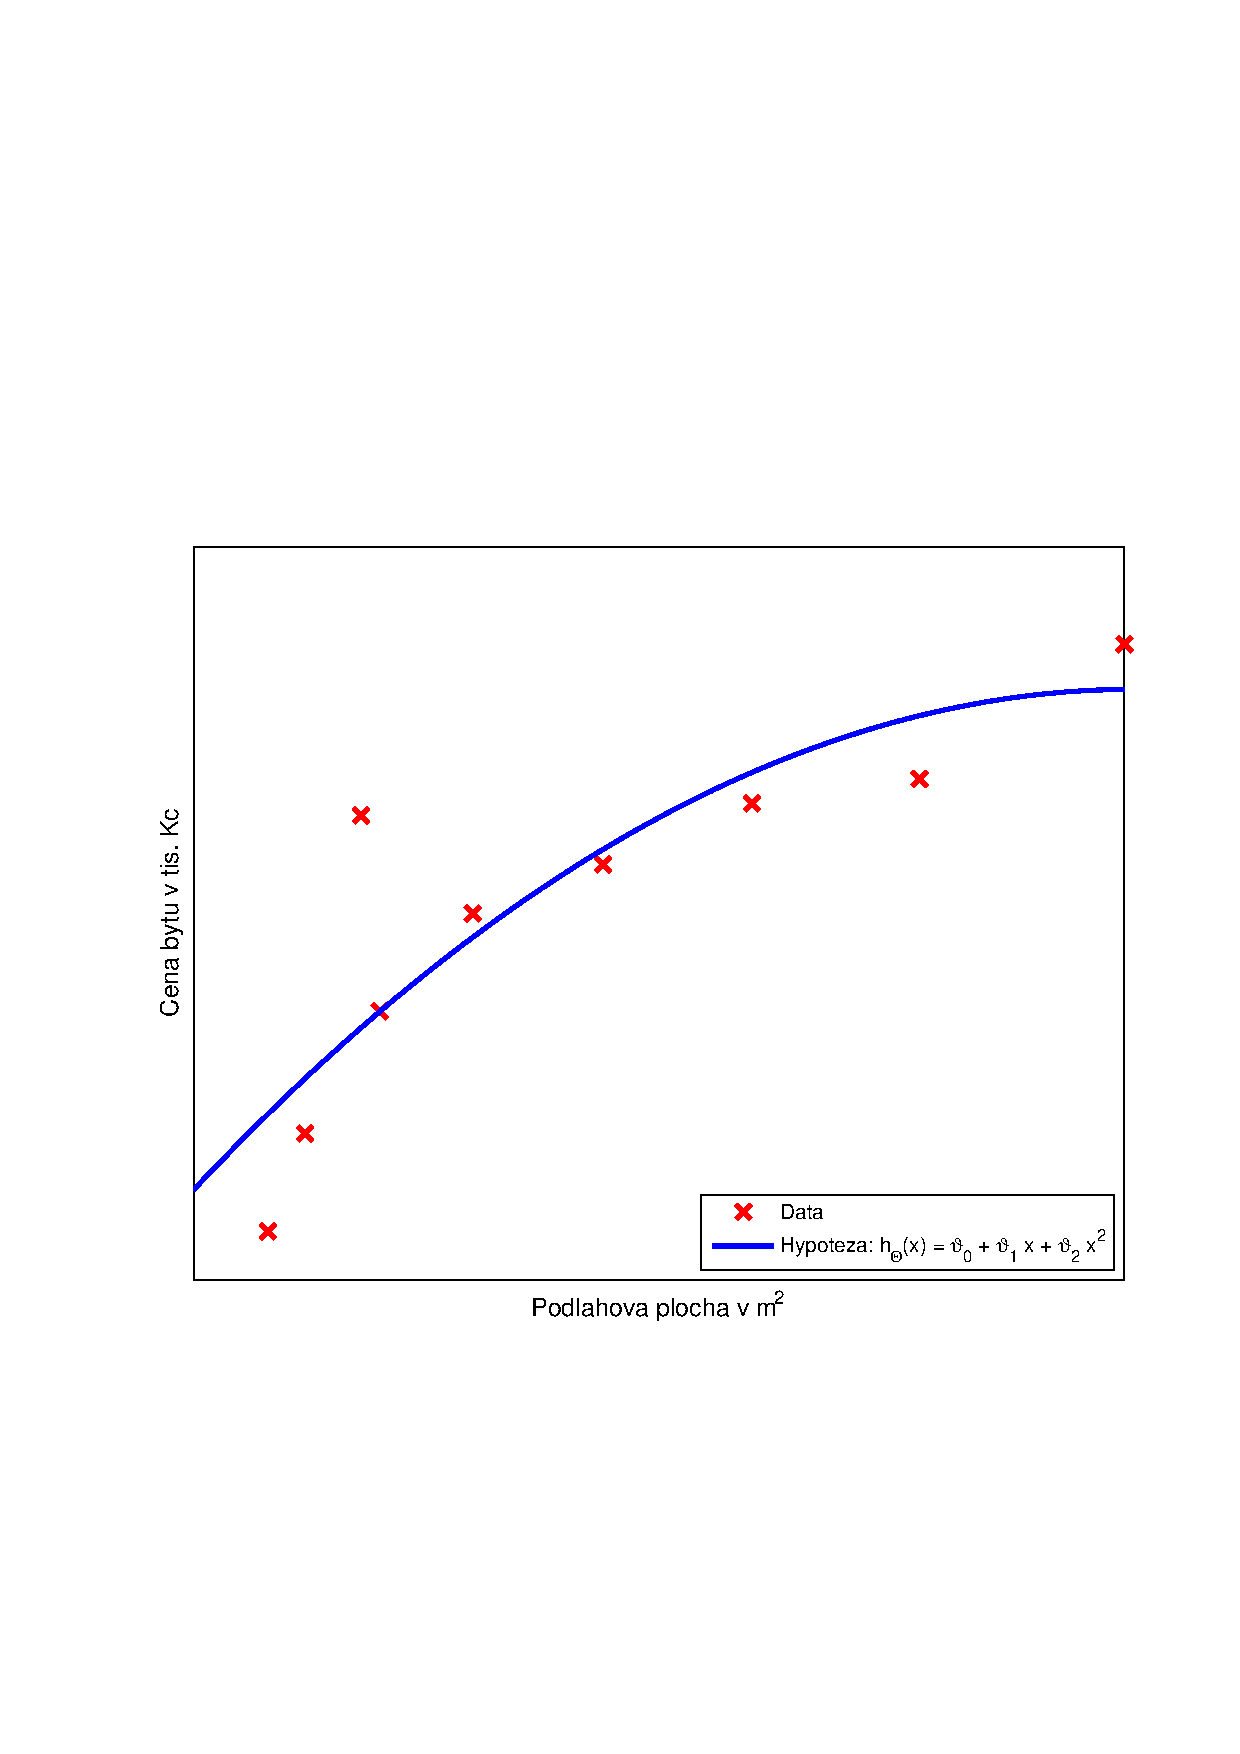
\includegraphics[width = \textwidth, trim = 2.5cm 7cm 2cm 9cm]{./Img/Regularizace/Pretrenovani1D/regrese_2.pdf}
  		\caption{Regrese pomocí hypotézy ve tvaru polynomu druhého stupně (\textit{just right}).}
	\end{minipage}%
	\hfill
	\begin{minipage}[t]{0.48\textwidth}
		%trim option's parameter order: left bottom right top
		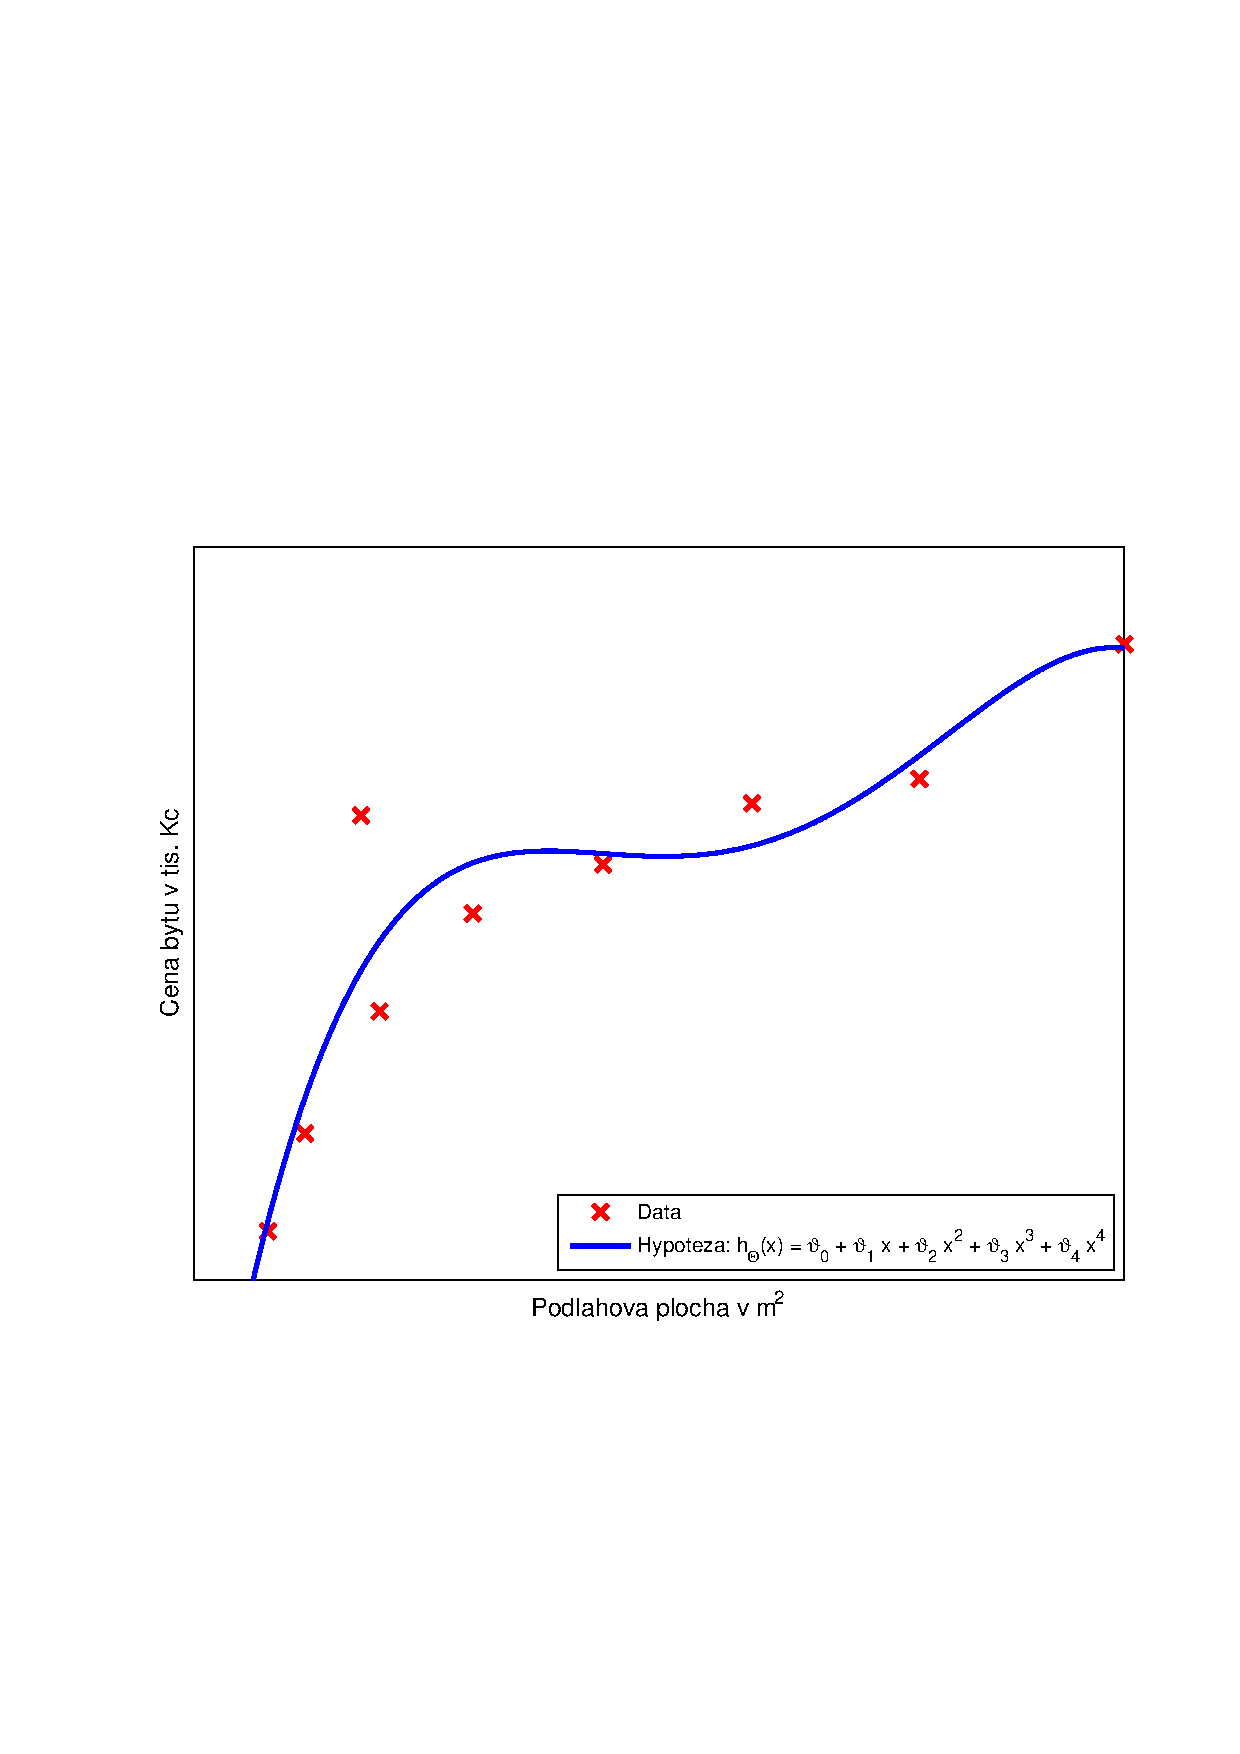
\includegraphics[width = \textwidth, trim = 2.5cm 7cm 2cm 9cm]{./Img/Regularizace/Pretrenovani1D/regrese_4.pdf}
  		\caption{Regrese pomocí hypotézy ve tvaru polynomu čtvrtého stupně (\textit{overfitting}, \textit{high variance}).}
	\end{minipage}%
\end{figure}

\par{Předpokládejme, že budeme penalizovat parametry $\vartheta_3$ a $\vartheta_4$ (jejich hodnoty budou malé). V rovnici \ref{eq:minZtratovaFunkce} je ukázána naše známá optimalizace
\begin{equation}
	\min_{\bm{\Theta}} \frac{1}{2m} \sum_{i=1}^{m} \left( h_{\bm{\Theta}} \left( \bm{x}^{\left( i \right)} \right) - y^{\left( i \right)} \right)^2,
	\label{eq:minZtratovaFunkce}
\end{equation}
kterou můžeme upravit na tvar
\begin{equation}
	\min_{\bm{\Theta}} \frac{1}{2m} \sum_{i=1}^{m} \left( h_{\bm{\Theta}} \left( \bm{x}^{\left( i \right)} \right) - y^{\left( i \right)} \right)^2 + 1000 \vartheta_3^2 + 1000 \vartheta_4^2,
	\label{eq:minZtratovaFunkce1000}
\end{equation}
kde hodnoty 1000 jsou pouze ilustrativní a~reprezentují velká čísla (velké váhy). Tedy pokud bychom chtěli minimalizovat rovnici \ref{eq:minZtratovaFunkce1000}, tak to lze za předpokladu, že $\vartheta_3$ a~$\vartheta_4$ budou malá čísla. V případě, že $\vartheta_3 \approx 0$ a $\vartheta_4 \approx 0$, tak získáme opět náš minimalizační problém jako v~rovnici \ref{eq:minZtratovaFunkce}. Ještě větší dopad to má na tvar hypotézy $h_{\bm{\Theta}} \left( \bm{x} \right) = \vartheta_0 + \vartheta_1 x + \vartheta_2 x^2 + \vartheta_2 x^3 + \vartheta_2 x^4$, která dříve vedla k přetrénování. Ta v~případě, že  $\vartheta_3 \approx 0$ a $\vartheta_4 \approx 0$ přejde na tvar $h_{\bm{\Theta}} \left( \bm{x} \right) = \vartheta_0 + \vartheta_1 x + \vartheta_2 x^2$. Tímto se zbavíme problému přetrénování a~získáme tvar hypotézy, který dobře zobecňuje trénovací data.}

\subsubsection*{Regularizace}
\par{Čím jsou menší hodnoty parametrů $\vartheta_0,\vartheta_1, \ldots , \vartheta_n$, tím \uv{jednodušší} tvar hypotézy získáme a tím méně je tvar hypotézy náchylný k přetrénování. Zapsáno rovnicí
\begin{equation}
	J \left( \bm{\Theta} \right) = \frac{1}{2m} \left( \sum_{i = 1}^{m} \left( h_{\bm{\Theta}} \left( \bm{x}^{\left( i \right)} \right) - y^{\left( i \right)} \right)^2 + \lambda \sum_{j = 1}^{n} \vartheta_j^2 \right),
\end{equation}
kde je nejdříve podotknout, že nová suma s indexem $j$ má jinou mez $n$ než první suma. To je způsobeno tím, že se regularizace vztahuje pouze na parametry $\vartheta_1, \vartheta_2, \ldots , \vartheta_m$, tedy parametr $\vartheta_0$ není regularizován, protože je vždy násoben jedničkou, nepřijde do kontaktu s~příznaky vzorků. Dále parametr $\lambda$ je takzvaný regularizační parametr, který kontroluje vyvážení mezi tím, jak hodně bude regularizace ovlivňovat původní ztrátovou funkci $J \left( \bm{\Theta} \right)$. Regularizace je dána vztahem 
\begin{equation}
	\lambda \sum_{j = 1}^{n} \vartheta_j^2.
\end{equation}
Našim cílem je jako dříve minimalizovat ztrátovou funkci
\begin{equation}
	\min_{\bm{\Theta}} J \left( \bm{\Theta} \right)
\end{equation}}

\par{Co se stane, pokud bude regularizační parametr $\lambda$ příliš velký? Řekněme, že $\lambda = 10^{10}$. Poté hypotéza ve tvaru $h_{\bm{\Theta}} \left( \bm{x} \right) = \vartheta_0 + \vartheta_1 x + \vartheta_2 x^2 + \vartheta_2 x^3 + \vartheta_2 x^4$ přejde na tvar $h_{\bm{\Theta}} \left( \bm{x} \right) = \vartheta_0$ a~výsledný průběh lze vidět na Obr.~\ref{fig:regularizaceUnderfit}}
\begin{figure}[!ht]
	\centering
	%trim option's parameter order: left bottom right top
	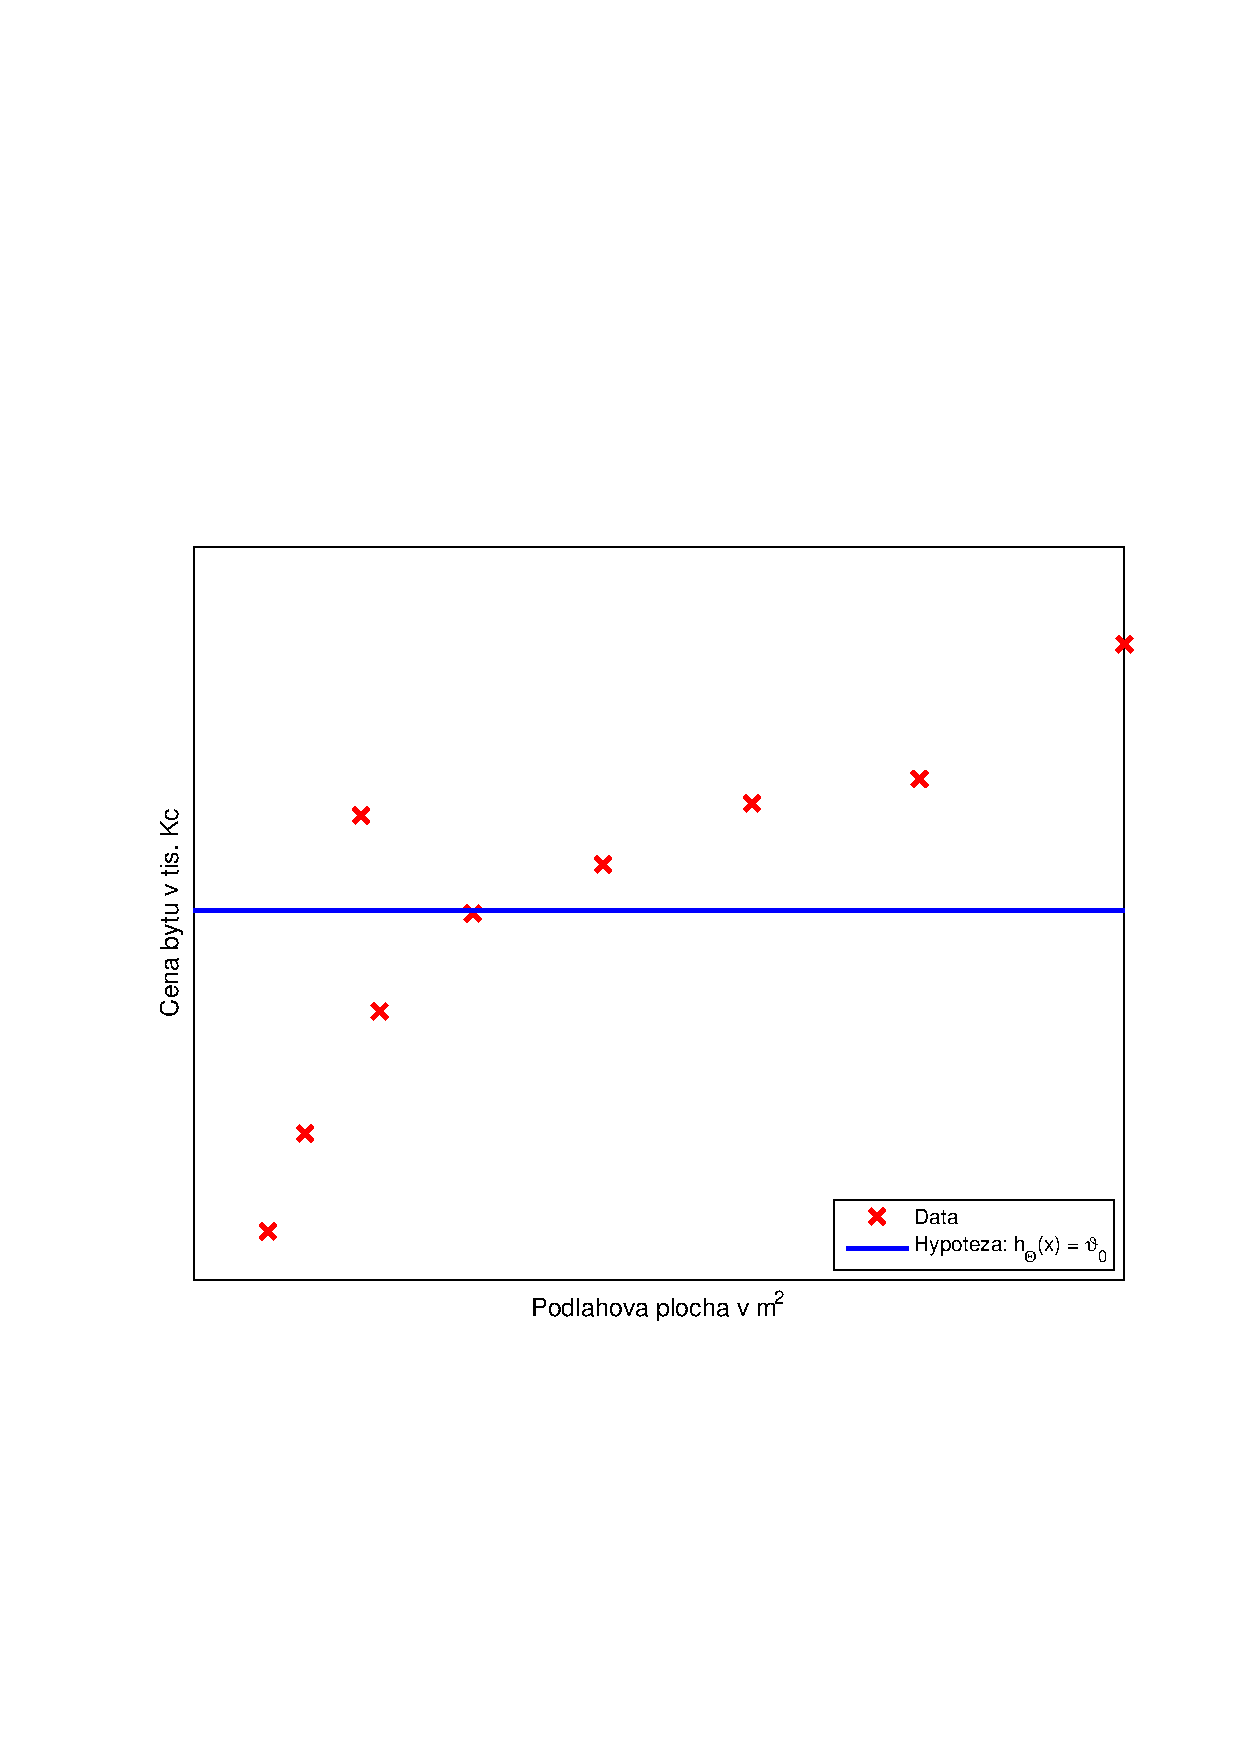
\includegraphics[width = 0.48\textwidth, trim = 2.5cm 7cm 2cm 9cm]{./Img/Regularizace/ZtratovaFunkce/regrese_underfit.pdf}
	\caption{Použití regularizace k získání \textit{underfit} hypotézy.}
	\label{fig:regularizaceUnderfit}
\end{figure}

\par{Z~uvedeného vyplývá, že je nutné volit regularizační parametr~$\lambda$ velmi opatrně. S~velkým~$\lambda$ dosáhneme \textit{underfit} problému a~s~malým~$\lambda$ neodstraníme \textit{overfit} problém.}

\newpage

















%----REGULARIZACE-LINEARNI-REGRESE--------------------------------------------------------------
\subsection{Regularizace lineární regrese}
\label{sec:RegularizaceLinearniRegrese}

\par{Pro lineární regresi máme odvozen gradientní algoritmus a analytické řešení. V této sekci oba algoritmy zobecníme s využitím regularizace.}


\subsubsection*{Regularizace gradientního algoritmu lineární regrese}
\par{Máme naší optimalizační úlohu lineární regrese společně s regularizací
\begin{equation}
	J \left( \bm{\Theta} \right) = \frac{1}{2m} \left( \sum_{i = 1}^{m} \left( h_{\bm{\Theta}} \left( \bm{x}^{\left( i \right)} \right) - y^{\left( i \right)} \right)^2 + \lambda \sum_{j = 1}^{n} \vartheta_j^2 \right),
\end{equation}
snažíme se minimalizovat ztrátovou funkci 
\begin{equation}
	\min_{\bm{\Theta}} J \left( \bm{\Theta} \right)
\end{equation}}

\par{Připomeňme si dříve představený gradientní algoritmus lineární regrese. Opakuj
\begin{equation}
	\vartheta_j = \vartheta_j - \alpha \frac{1}{m} \sum_{i = 1}^{m} \left( h_{\bm{\Theta}} \left( \bm{x}^{\left( i \right)} \right) - y^{\left( i \right)} \right) x_j^{\left( i \right)}, \quad j = 0,1,\ldots ,n .
\end{equation}
Tento algoritmus je možno rozdělit do dvou kroků. Rozdělit výpočet pro $\vartheta_0$ a $\vartheta_{1,\ldots, n}$. Opakuj
\begin{eqnarray}
	&\vartheta_0 &= \vartheta_0 - \alpha \frac{1}{m} \sum_{i = 1}^{m} \left( h_{\bm{\Theta}} \left( \bm{x}^{\left( i \right)} \right) - y^{\left( i \right)} \right) x_0^{\left( i \right)},\\
	%
	&\vartheta_j &= \vartheta_j - \alpha \frac{1}{m} \sum_{i = 1}^{m} \left( h_{\bm{\Theta}} \left( \bm{x}^{\left( i \right)} \right) - y^{\left( i \right)} \right) x_j^{\left( i \right)}, \quad j = 1,2,\ldots ,n .
\end{eqnarray}
Doposud na algoritmu nebylo nic změněno, pouze byl rozepsán do dvou kroků. Protože víme, že na parametr $\vartheta_0$ se regularizace nevztahuje, proto můžeme algoritmus pozměnit a přidat regularizační člen. Následně bude mít gradientní algoritmus tvar. Opakuj
\begin{eqnarray}
	&\vartheta_0 &= \vartheta_0 - \alpha \frac{1}{m} \sum_{i = 1}^{m} \left( h_{\bm{\Theta}} \left( \bm{x}^{\left( i \right)} \right) - y^{\left( i \right)} \right) x_0^{\left( i \right)},\\
		%
	&\vartheta_j &= \vartheta_j - \alpha \left( \frac{1}{m} \sum_{i = 1}^{m} \left( h_{\bm{\Theta}} \left( \bm{x}^{\left( i \right)} \right) - y^{\left( i \right)} \right) x_j^{\left( i \right)} + \frac{\lambda}{m} \vartheta_j \right), \quad j = 1,2,\ldots ,n,	
	\label{eq:LinearniRegreseGradientniAlgProJ1}
\end{eqnarray}
kde platí
\begin{eqnarray}
	\frac{\partial}{\partial \vartheta_0} &J \left( \bm{\Theta} \right)	&= \left( \frac{1}{m} \sum_{i = 1}^{m} \left( h_{\bm{\Theta}} \left( \bm{x}^{\left( i \right)} \right) - y^{\left( i \right)} \right) x_0^{\left( i \right)} \right),\\
	%
	\frac{\partial}{\partial \vartheta_j} &J \left( \bm{\Theta} \right) &= \left( \frac{1}{m} \sum_{i = 1}^{m} \left( h_{\bm{\Theta}} \left( \bm{x}^{\left( i \right)} \right) - y^{\left( i \right)} \right) x_j^{\left( i \right)} + \frac{\lambda}{m} \vartheta_j \right), \quad j = 1,2,\ldots ,n.
\end{eqnarray}}

\par{Rovnice \ref{eq:LinearniRegreseGradientniAlgProJ1} lze přepsat do tvaru 
\begin{equation}
	\vartheta_j = \vartheta_j \left( 1 - \alpha \frac{\lambda}{m} \right) - \alpha \frac{1}{m} \sum_{i = 1}^{m} \left( h_{\bm{\Theta}} \left( \bm{x}^{\left( i \right)} \right) - y^{\left( i \right)} \right) x_j^{\left( i \right)},
\end{equation}
kde platí
\begin{equation}
	1 - \alpha \frac{\lambda}{m} < 1.
\end{equation}}



\subsubsection*{Regularizace analytického řešení lineární regrese}

\par{Připomeňme si}
\begin{equation}
	\bm{X} = \left[ \left( \bm{x}^{\left( 1 \right)} \right)^{\top}, \ldots, \left( \bm{x}^{\left( m \right)} \right)^{\top}  \right]^{\top},\quad  \bm{X} \in  \mathcal{R}^{m \times \left( n + 1 \right)}
\end{equation}
a
\begin{equation}
	\bm{y} = \left[ y^{\left( 1 \right)}, \ldots, y^{\left( m \right)}   \right]^{\top}, \quad \bm{y} \in \mathcal{R}^{m}.
\end{equation}
Analytické řešení pro výpočet $\bm{\Theta}$ má tvar
\begin{equation}
	\bm{\Theta} = \left( \bm{X}^{\top} \bm{X} \right)^{-1} \bm{X}^{\top} y.
\end{equation}
Cílem je minimalizovat ztrátovou funkci
\begin{equation}
	\min_{\bm{\Theta}} J \left( \bm{\Theta} \right).
\end{equation}

\par{Pokud využijeme regularizaci, tak naše analytické řešení přejde na tvar
\begin{equation}
	\bm{\Theta} = \left( \bm{X}^{\top} \bm{X} + \lambda 
	\left[ \begin{array}{ccccc}
		0 & 0 & 0 & 0 & 0\\
		0 & 1 & 0 & 0 & 0 \\
		0 & 0 & 1 & 0 & 0\\
		0 & 0 & 0 & \ddots & \vdots\\
		0 & 0 & 0 & \cdots & 1
	\end{array} \right] \right)^{-1} \bm{X}^{\top} y
\end{equation}
kde nová matice má velikost $\mathcal{R}^{\left( n + 1 \right) \times \left( n+ 1 \right)}$}

\subsubsection*{Rozšíření}
\par{Předpokládejme, že $m \leq n$, kde $m$ je počet vzorků a $n$ je počet příznaků a 
\begin{equation}
	\bm{\Theta} = \left( \bm{X}^{\top} \bm{X} \right)^{-1} \bm{X}^{\top} y,
\end{equation}
pak je matice $\bm{X}^{\top} \bm{X} $ neinvertovatelná / singulární.}

\par{Pro výpočet lze v tomto případě využít pseudoinverze, konkrétně v~MATLABu k~tomuto účelu slouží funkce \textit{pinv()}.}
\lstinputlisting[language = Matlab]{./Img/Regularizace/noninvertibilityXX/XX.m}

\par{Pokud $\lambda > 0$}
\begin{equation}
	\bm{\Theta} = \left( \underbrace{ \bm{X}^{\top} \bm{X} + \lambda 
	\left[ \begin{array}{ccccc}
		0 & ~ & ~ & ~ & ~\\
		~ & 1 & ~ & ~ & ~ \\
		~ & ~ & 1 & ~ & ~\\
		~ & ~ & ~ & \ddots & ~\\
		~ & ~ & ~ & ~ & 1
	\end{array} \right]}_{\text{Matice musí být invertovatelná}}  \right)^{-1} \bm{X}^{\top} y
\end{equation}

\newpage






















%----REGULARIZACE-BINARNI REGRESE--------------------------------------------------------------
\subsection{Regularizace binární regrese}
\par{Pro binární regresi jsme dříve mluvili o dvou typech optimalizace. Mluvili jsme o tom, jak použít gradientní algoritmus a jak použít pokročilé metody optimalizace. V této sekci si ukážeme, jak tyto přístupy upravit, aby využily regularizace.}

\subsubsection*{Regularizace binární regrese}

\par{Dříve jsme si ukázali, že binární regrese je náchylná na přetrénování v případě, kdy zvolíme vysoký stupeň polynomu reprezentující naší hypotézu, například
\begin{equation}
	h_{\bm{\Theta}} \left( \bm{x} \right) = g \left( \vartheta_0  + \vartheta_1 x_1 + \vartheta_2 x^2_1 + \vartheta_3 x_1^2 x_2 + \vartheta_4 x_1^2 x_2^2 + \vartheta_5 x_1^2 x_2^3 + \ldots \right),
	\label{eq:BReg_hypo}
\end{equation}
pro takovouto složitou hypotézu můžeme dostat dělící křivku velmi variabilní a velmi respektující rozdělení trénovacích dat, tedy křivku, která nedostatečně zobecňuje.
\begin{figure}[!ht]
	\centering
	%trim option's parameter order: left bottom right top
	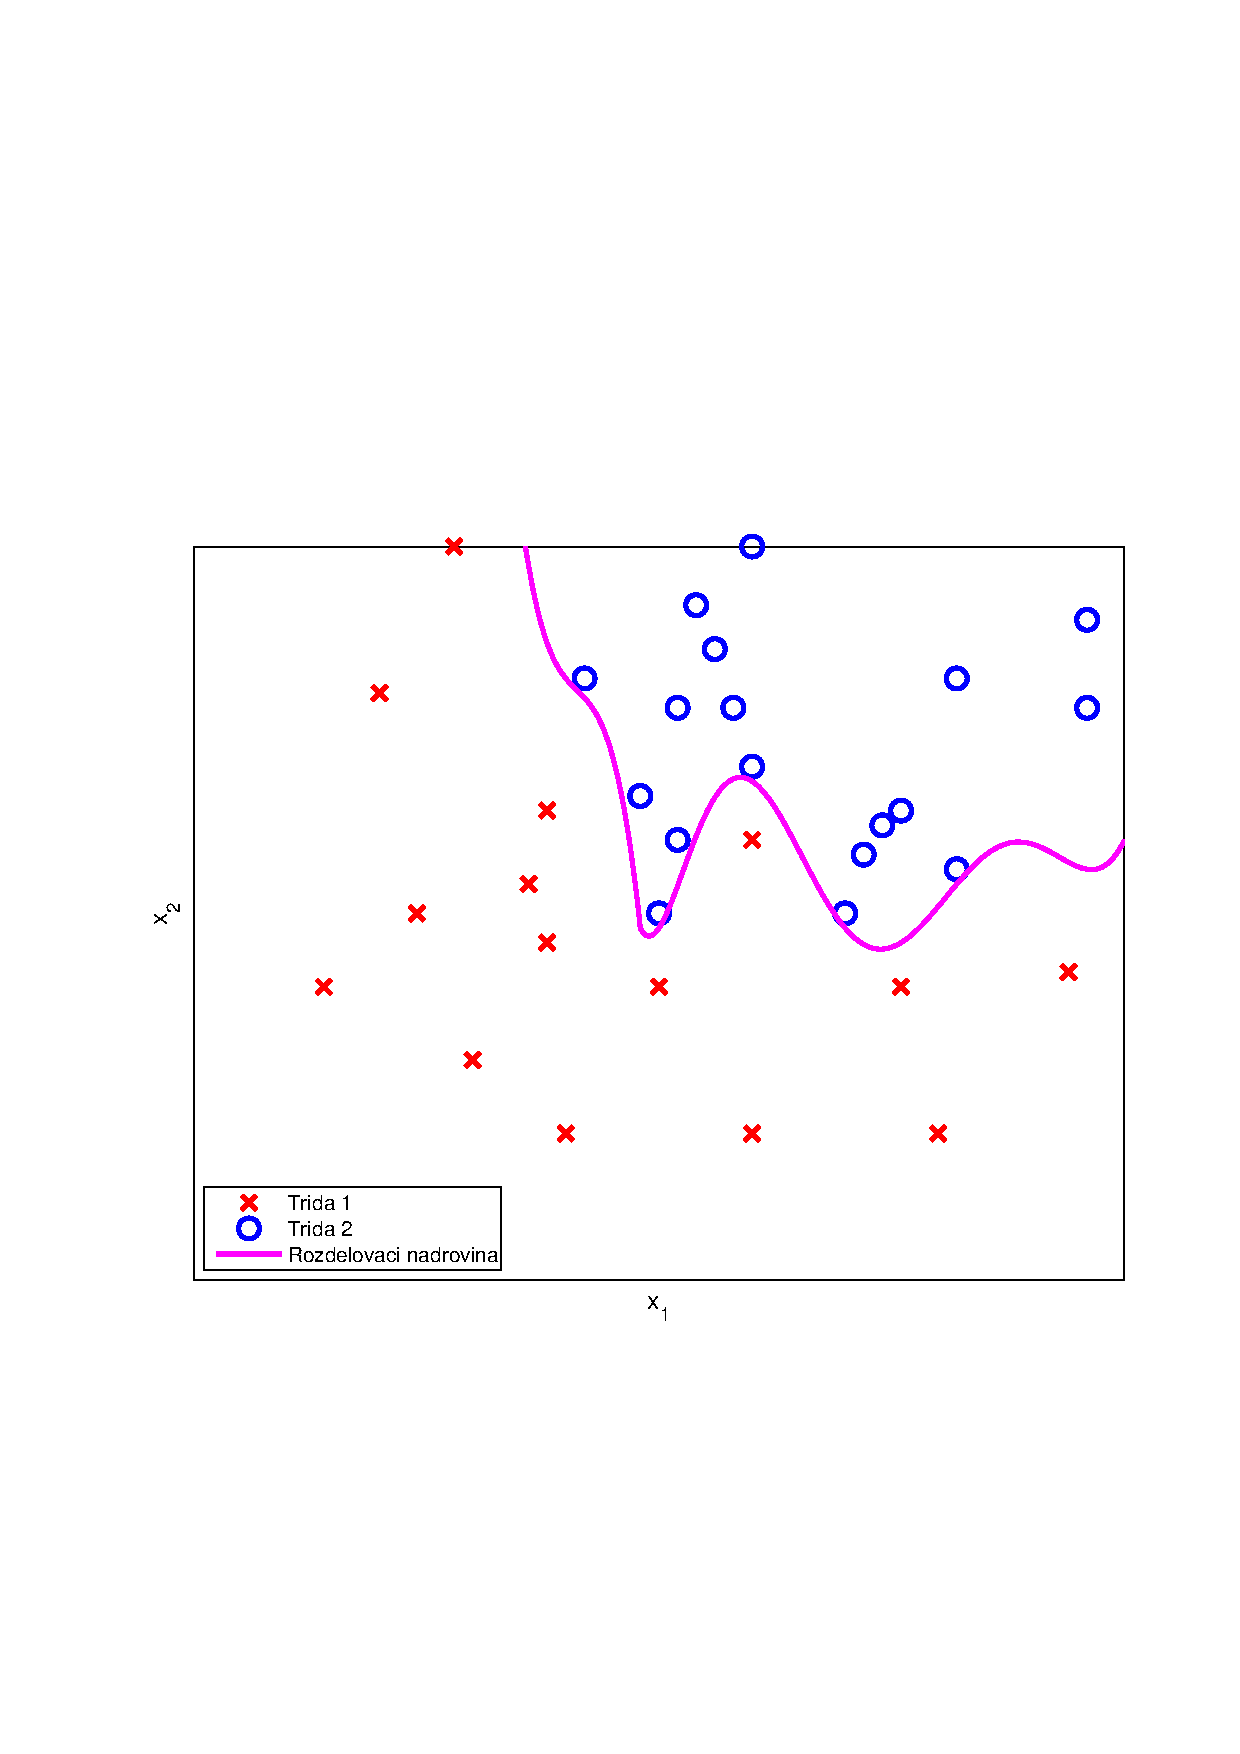
\includegraphics[width = 0.48\textwidth, trim = 2.5cm 7cm 2cm 9cm]{./Img/Regularizace/binarniRegrese/regularizace_binarni_regrese.pdf}
	\caption{Možný výsledek s použitím hypotézy z rovnice \ref{eq:BReg_hypo}.}
	\label{fig:binaryRegularizationExample}
\end{figure}
}

\par{Ztrátová funkce pro binární regresi má tvar
\begin{equation}
	J \left( \bm{\Theta} \right) =  - \left[ \frac{1}{m} \sum_{i = 1}^{m} y^{ \left( i \right)} \log \left( h_{\bm{\Theta}} \left( \bm{x}^{\left( i \right)} \right) \right) + \left( 1 - y^{\left( i \right)} \right) \log \left( 1 - h_{\bm{\Theta}} \left( \bm{x}^{\left( i \right)} \right) \right) \right]
\end{equation}
a její modifikací získáme regularizovaný tvar ztrátové funkce
\begin{equation}
	J \left( \bm{\Theta} \right) =  - \left[ \frac{1}{m} \sum_{i = 1}^{m} y^{ \left( i \right)} \log \left( h_{\bm{\Theta}} \left( \bm{x}^{\left( i \right)} \right) \right) + \left( 1 - y^{\left( i \right)} \right) \log \left( 1 - h_{\bm{\Theta}} \left( \bm{x}^{\left( i \right)} \right) \right) \right] + \frac{\lambda}{2m} \sum_{j = 1}^{n} \vartheta_j^2
\end{equation}
přidaná suma je jen do $n$, jelikož se neregularizuje složka $\vartheta_0$, která je vždy rovna jedné a~není v~součinu se žádnou proměnnou $x$, $y$. Tvar ztrátové funkce společně s~regularizací bude naší rozdělovací nadrovinu více zobecňovat a~pomůže nám řešit problém přetrénování.}

\par{Implementace bude provedena následovně: opakuj
\begin{eqnarray}
	&\vartheta_0 &= \vartheta_0 - \alpha \frac{1}{m} \sum_{i = 1}^{m} \left( h_{\bm{\Theta}} \left( \bm{x}^{\left( i \right)} \right) - y^{\left( i \right)} \right) x_0^{\left( i \right)}\\
	&\vartheta_j &= \vartheta_j - \alpha \left[ \frac{1}{m} \sum_{i = 1}^{m} \left( h_{\bm{\Theta}} \left( \bm{x}^{\left( i \right)} \right) - y^{\left( i \right)} \right) x_j^{\left( i \right)} + \frac{\lambda}{m} \vartheta_j \right], \qquad j = 1, 2, 3, \ldots , n,
	\label{eq:gradDescent_regularizace2rce}
\end{eqnarray}
kde 
\begin{equation}
	h_{\bm{\Theta}} \left( \bm{x} \right) = \frac{1}{1 + e^{- \bm{\Theta}^{\top} \bm{x} }}.
\end{equation}
Z~rovnice \ref{eq:gradDescent_regularizace2rce} lze vidět, že platí
\begin{equation}
	\frac{\partial}{\partial \vartheta_j} J \left( \bm{\Theta} \right) = \frac{1}{m} \sum_{i = 1}^{m} \left( h_{\bm{\Theta}} \left( \bm{x}^{\left( i \right)} \right) - y^{\left( i \right)} \right) x_j^{\left( i \right)} + \frac{\lambda}{m} \vartheta_j.
\end{equation}}





\subsubsection*{Regularizace pokročilé optimalizace}
\par{Nyní bude nastíněno jak využit pokročilé optimalizace v MATLABu. Nechť náš vektor parametrů $\bm{\Theta}$ odpovídá
\begin{equation}
	\bm{\Theta} = \left[ \vartheta_0 , \vartheta_1, \ldots , \vartheta_n \right]^{\top} = \left[ theta(1), theta(2), \ldots, theta(n + 1 ) \right]
\end{equation}
(z důvodu, že MATLAB indexuje od jedničky).
\lstinputlisting[language = Matlab]{./Img/Regularizace/AdvancedOptimalization/costFunction.m}
\begin{equation}
	J \left( \bm{\Theta} \right) = \left[ 
	- \frac{1}{m} \sum_{i = 1}^{m} y^{\left( i \right)} 
	\log \left( h_{\bm{\Theta}} \left( \bm{x}^{\left( i \right) } \right) \right)
	+ \left( 1 - y^{\left( i \right)} \right)
	\log \left( 1 - h_{\bm{\Theta}} \left( \bm{x}^{\left( i \right)} \right) \right) \right] + \frac{\lambda}{2m} \sum_{j = 1}^{n} \vartheta_j^2
\end{equation}
dále výpočet gradientu
\lstinputlisting[language = Matlab]{./Img/Regularizace/AdvancedOptimalization/grad1.m}
\begin{equation}
	\frac{\partial}{\partial \vartheta_0} J \left( \bm{\Theta} \right) = \frac{1}{m} \sum_{i = 1}^{m} \left( h_{\bm{\Theta}} \left( \bm{x}^{\left( i \right)} \right) - y^{\left( i \right)} \right) x_0^{\left( i \right)},
\end{equation}
\lstinputlisting[language = Matlab]{./Img/Regularizace/AdvancedOptimalization/grad2.m}
\begin{equation}
	\frac{\partial}{\partial \vartheta_1} J \left( \bm{\Theta} \right) = \left[ \frac{1}{m} \sum_{i = 1}^{m} \left( h_{\bm{\Theta}} \left( \bm{x}^{\left( i \right)} \right) - y^{\left( i \right)} \right) x_1^{\left( i \right)} \right] + \frac{\lambda}{m} \vartheta_1,
\end{equation}
\lstinputlisting[language = Matlab]{./Img/Regularizace/AdvancedOptimalization/grad3.m}
\begin{equation}
	\frac{\partial}{\partial \vartheta_2} J \left( \bm{\Theta} \right) = \left[ \frac{1}{m} \sum_{i = 1}^{m} \left( h_{\bm{\Theta}} \left( \bm{x}^{\left( i \right)} \right) - y^{\left( i \right)} \right) x_2^{\left( i \right)} \right] + \frac{\lambda}{m} \vartheta_2,
\end{equation}
\lstinputlisting[language = Matlab]{./Img/Regularizace/AdvancedOptimalization/gradN+1.m}
\begin{equation}
	\ldots
\end{equation}}






\newpage























\chapter{Neuronové sítě}

\section{Nelineární hypotézy}
\section{Neurony a lidský mozek}
\section{Reprezentace modelu}
\section{Příklady}
\section{Klasifikace do více tříd}


\chapter{Neuronové sítě učení}

\section{Ztrátová funkce}
\section{Algoritmus zpětného šíření chyby}
\section{Gradient Checking}
\section{Náhodná inicializace}
\section{Příklady}


\chapter{Suport Vector Machine (SVM)}
\label{sec:SVM}

\section{Cíl optimalizace}

\section{Large margin}

\section{Mathematic Behind Large Margin Classification}

\section{Kernels / Jádra}

\section{Kernel Trick}
Bowl $x^2 + y^2$

\section{Použití SVM}


\chapter{Shlukování}
\label{sec:shlukovani}

\par{V této kapitole bude popsáno učení bez učitele, algoritmus K-Means, cíl optimalizace, náhodná inicializace a volba počtu shluků.}









\section{Učení bez učitele}

\subsubsection*{Učení s učitelem}
\par{Typický problém učení s učitelem, kdy máme množinu vzorků $\bm{x}$ a k nim odpovídající informaci od učitele $y$. Trénovací množina má strukturu
\begin{equation}
	\left\lbrace \left( \bm{x}^{\left( 1 \right)} , y^{\left( 1 \right)} \right), \left( \bm{x}^{\left( 2 \right)} , y^{\left( 2 \right)} \right),  \left( \bm{x}^{\left( 3 \right)} , y^{\left( 3 \right)} \right), \ldots,  \left( \bm{x}^{\left( m \right)} , y^{\left( m \right)} \right) \right\rbrace .
\end{equation}
cílem je nalézt dělící nadrovinu, která bude nejlépe klasifikovat do dvou tříd.
\begin{figure}[!ht]
	\centering
	\begin{minipage}[t]{0.48\textwidth}
  		%trim option's parameter order: left bottom right top
		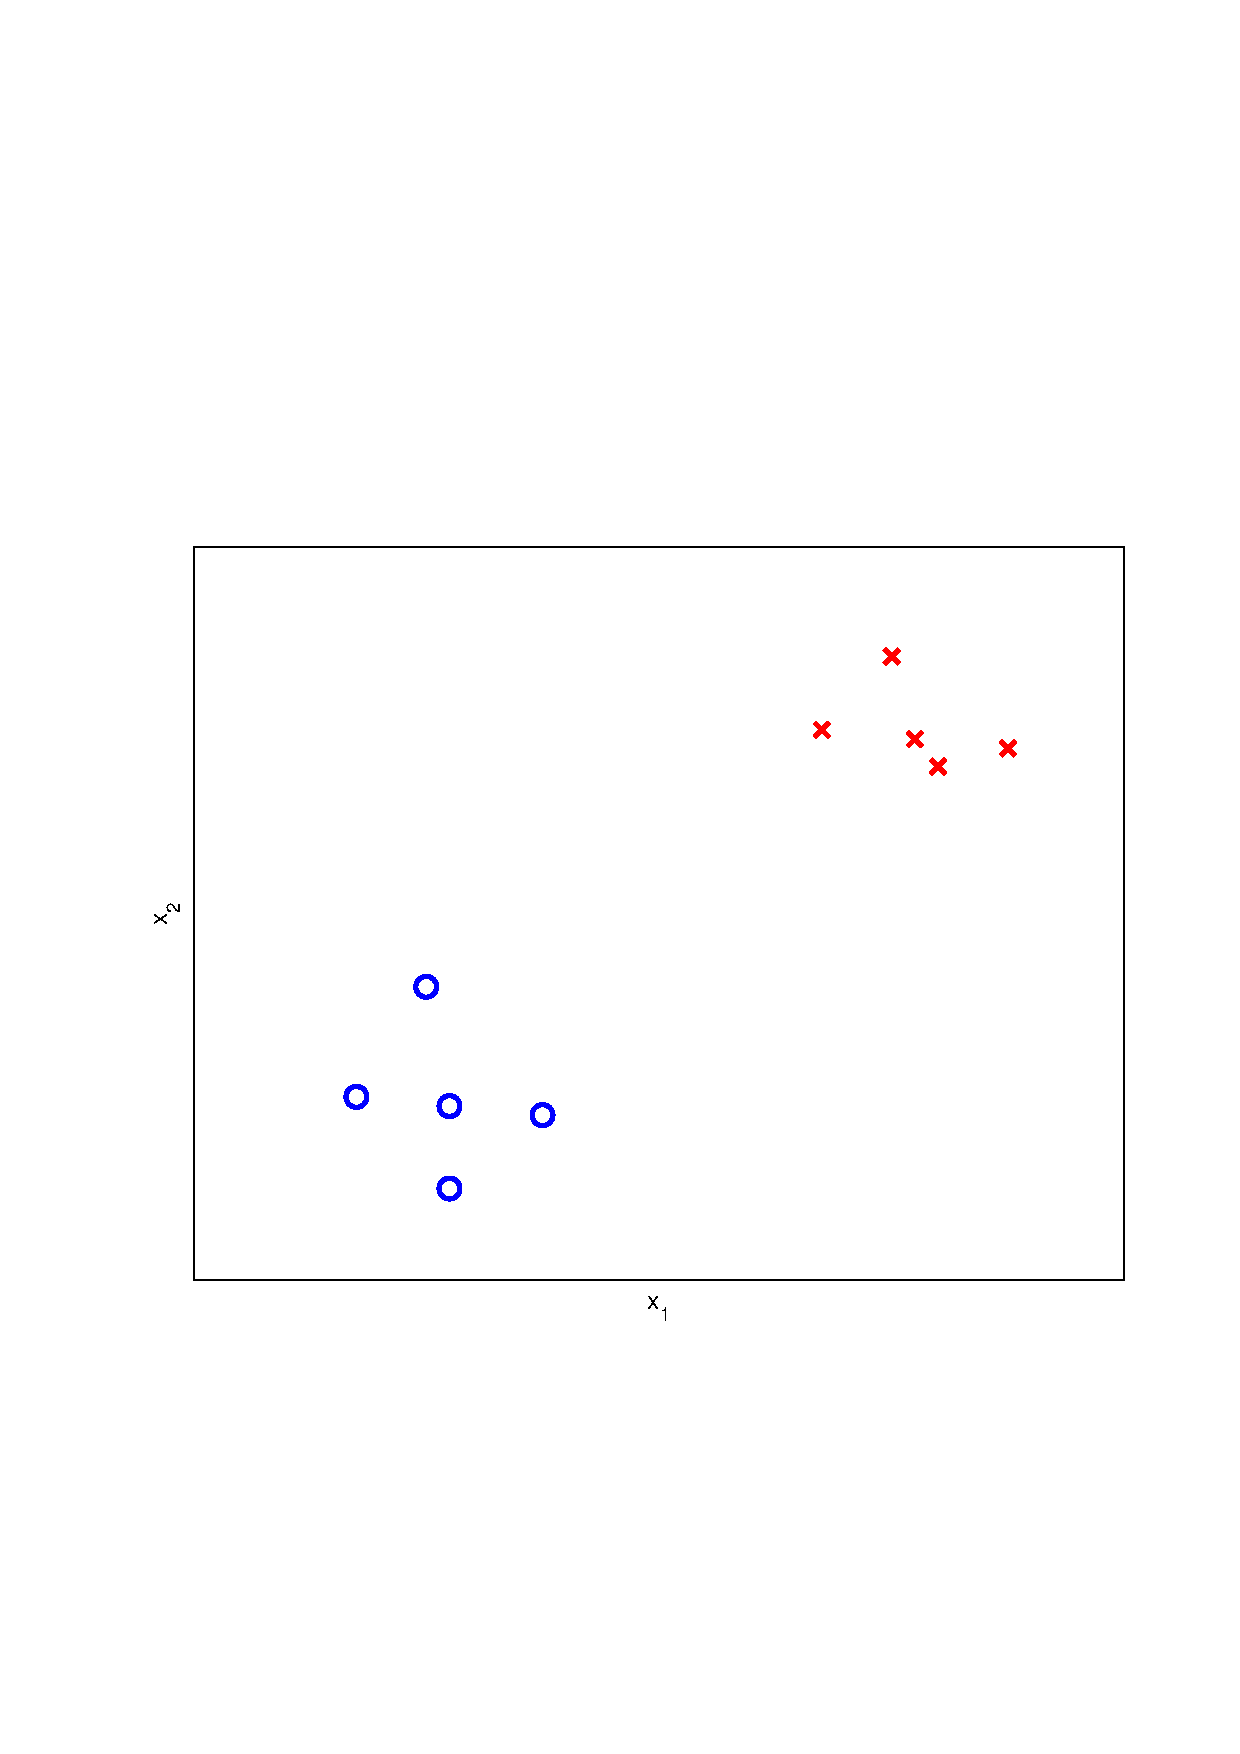
\includegraphics[width = \textwidth, trim = 2.5cm 7cm 2cm 9cm]{./Img/UnsupervizedLearning/Intro/supervized.pdf}
  		\caption{Klasifikace do dvou tříd - učení s učitelem.}
		\label{fig:supervized}
	\end{minipage}%
	\hfill
	\begin{minipage}[t]{0.48\textwidth}
		%trim option's parameter order: left bottom right top
		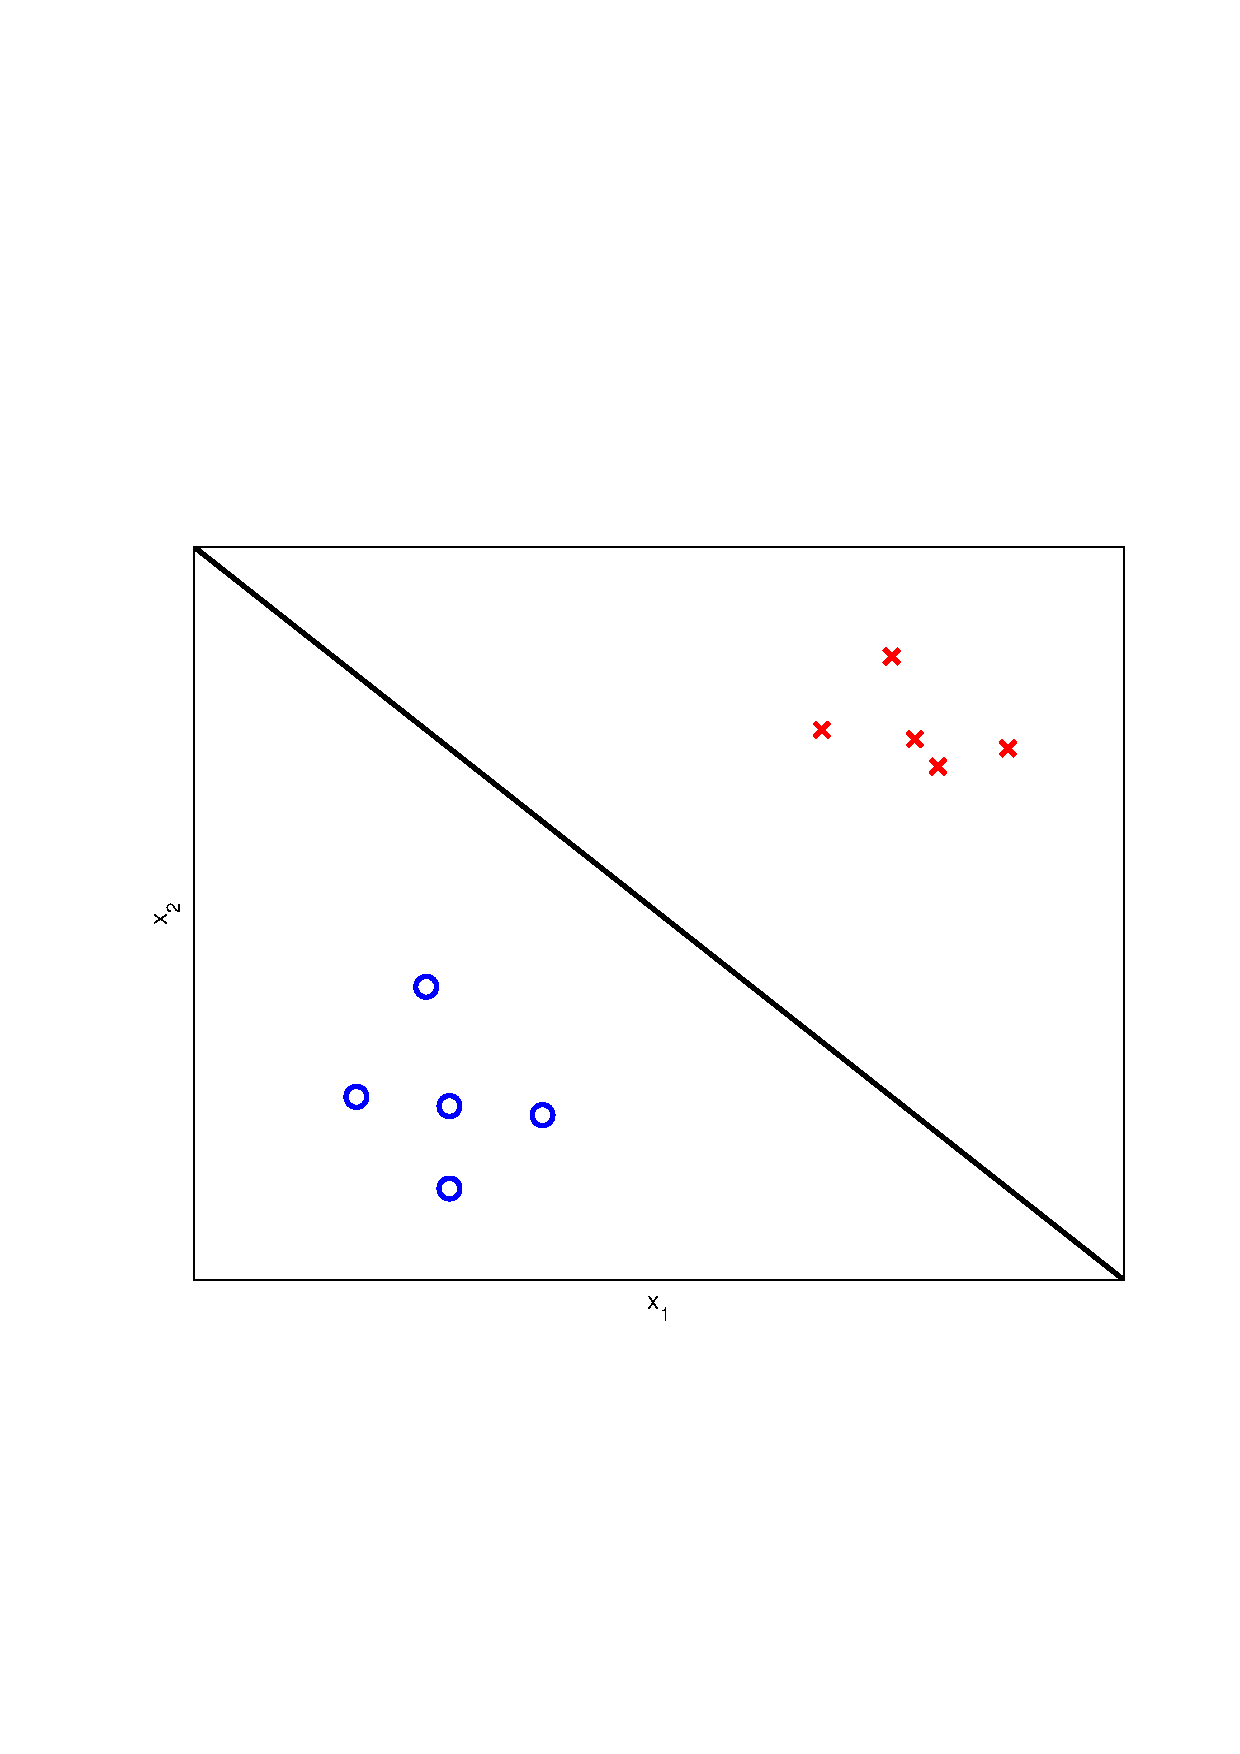
\includegraphics[width = \textwidth, trim = 2.5cm 7cm 2cm 9cm]{./Img/UnsupervizedLearning/Intro/supervized_line.pdf}
  		\caption{Klasifikace do dvou tříd s~dělící nadrovinou - učení s~učitelem.}
		\label{fig:supervized_line}
	\end{minipage}%
\end{figure}}

\par{Na Obr.~\ref{fig:supervized} a~\ref{fig:supervized_line} barva a~znak (kolečko nebo křížek) reprezentuje informaci od učitele.}

\newpage




\subsubsection*{Učení bez učitele}
\par{
V~případě učení bez učitele nemáme informaci od učitele do jaké třídy daný vzor patří. Trénovací množina má proto tvar
\begin{equation}
		\left\lbrace \bm{x}^{\left( 1 \right)} ,  \bm{x}^{\left( 2 \right)},   \bm{x}^{\left( 3 \right)} ,  \ldots,  \bm{x}^{\left( m \right)} \right\rbrace ,
\end{equation}
cílem učícího se algoritmu je nalézt strukturu mezi neznámými daty a~klasifikovat jednotlivé vzory do odpovídajících tříd. Je zřejmé, že v případě učení bez učitele postrádáme důležitou informaci o~počtu tříd. V~extrémních případech může být počet tříd roven jedné a~nebo počtu trénovacích vzorů. Na Obr.~\ref{fig:unsupervized}} a~\ref{fig:unsupervized_circle} lze vidět, že informace od učitele ve formě barvy a~znaku chybí.
\begin{figure}[!ht]
	\centering
	\begin{minipage}[t]{0.48\textwidth}
  		%trim option's parameter order: left bottom right top
		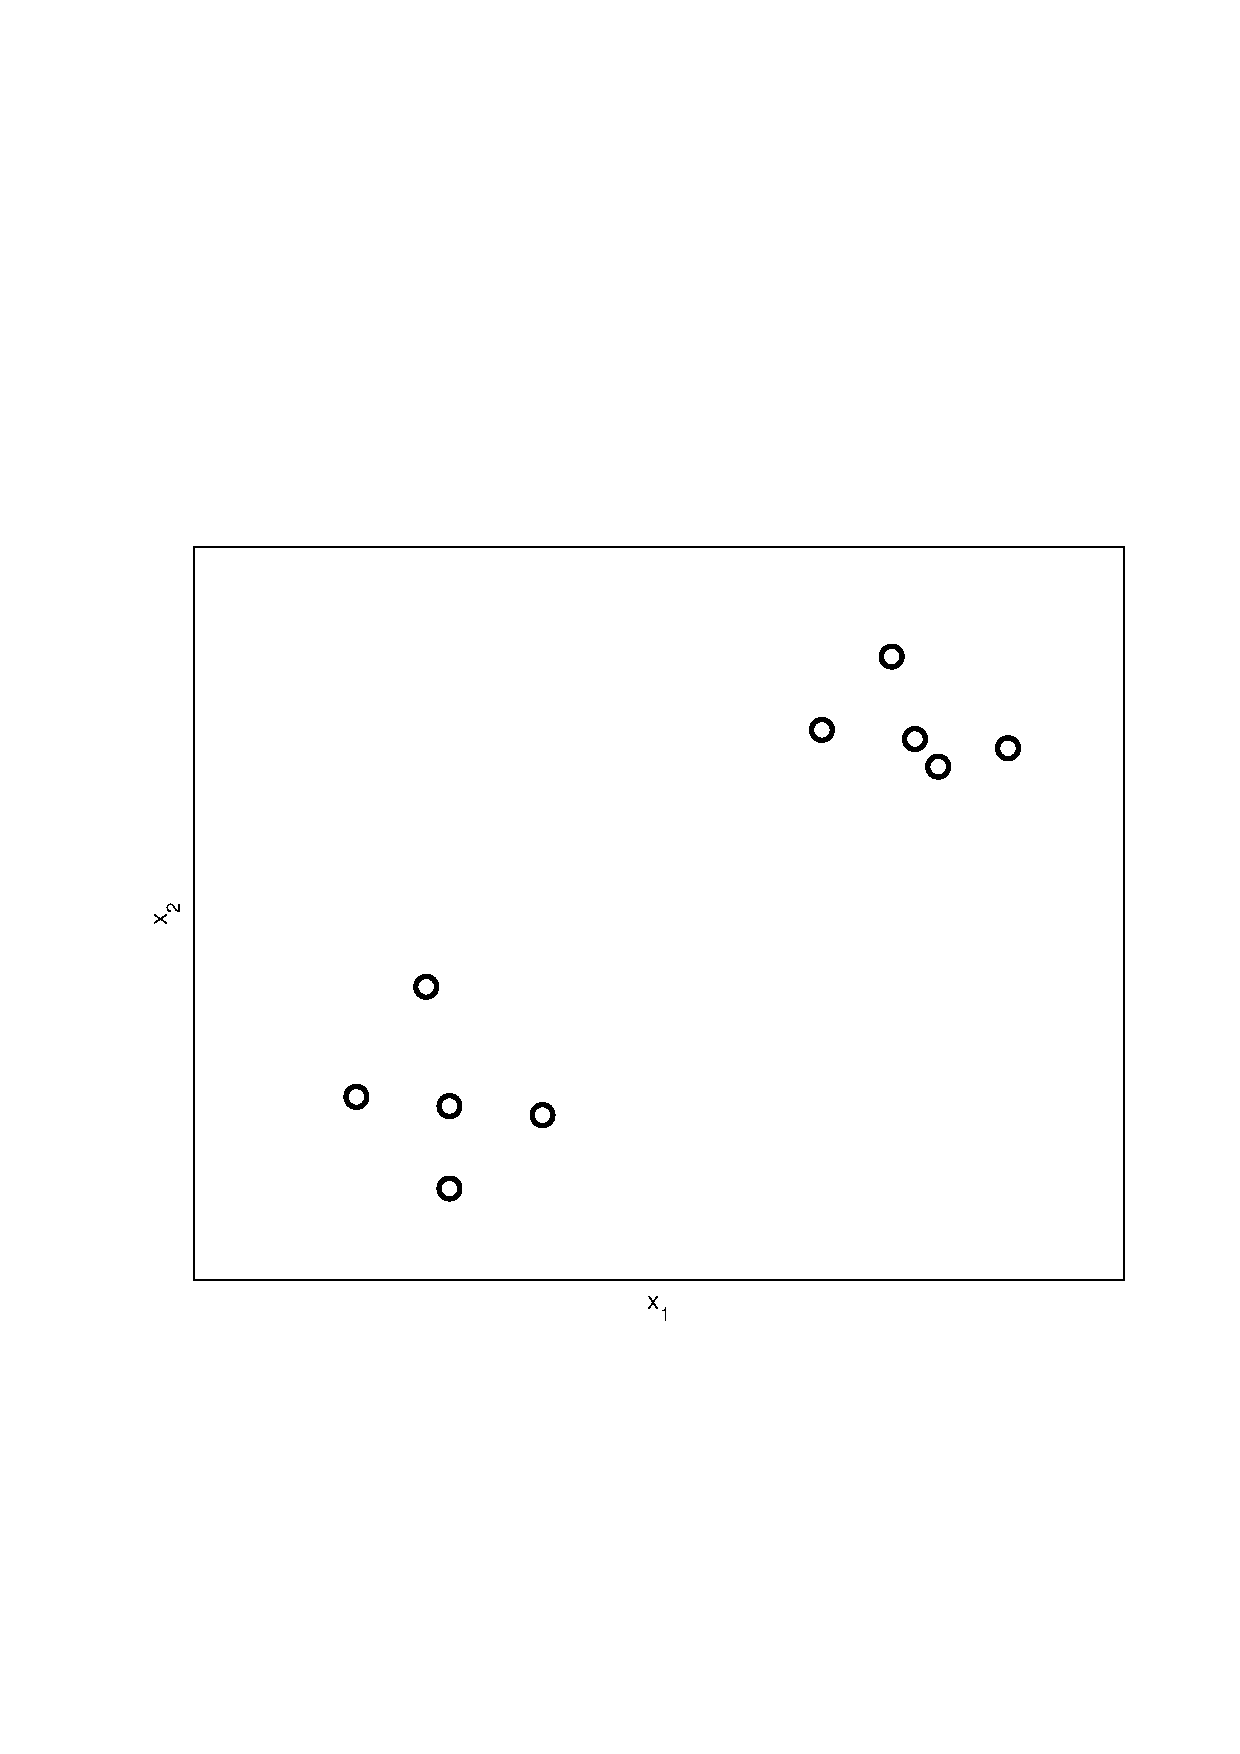
\includegraphics[width = \textwidth, trim = 2.5cm 7cm 2cm 9cm]{./Img/UnsupervizedLearning/Intro/unsupervized.pdf}
  		\caption{Klasifikace do dvou tříd - učení bez učitele.}
		\label{fig:unsupervized}
	\end{minipage}%
	\hfill
	\begin{minipage}[t]{0.48\textwidth}
		%trim option's parameter order: left bottom right top
		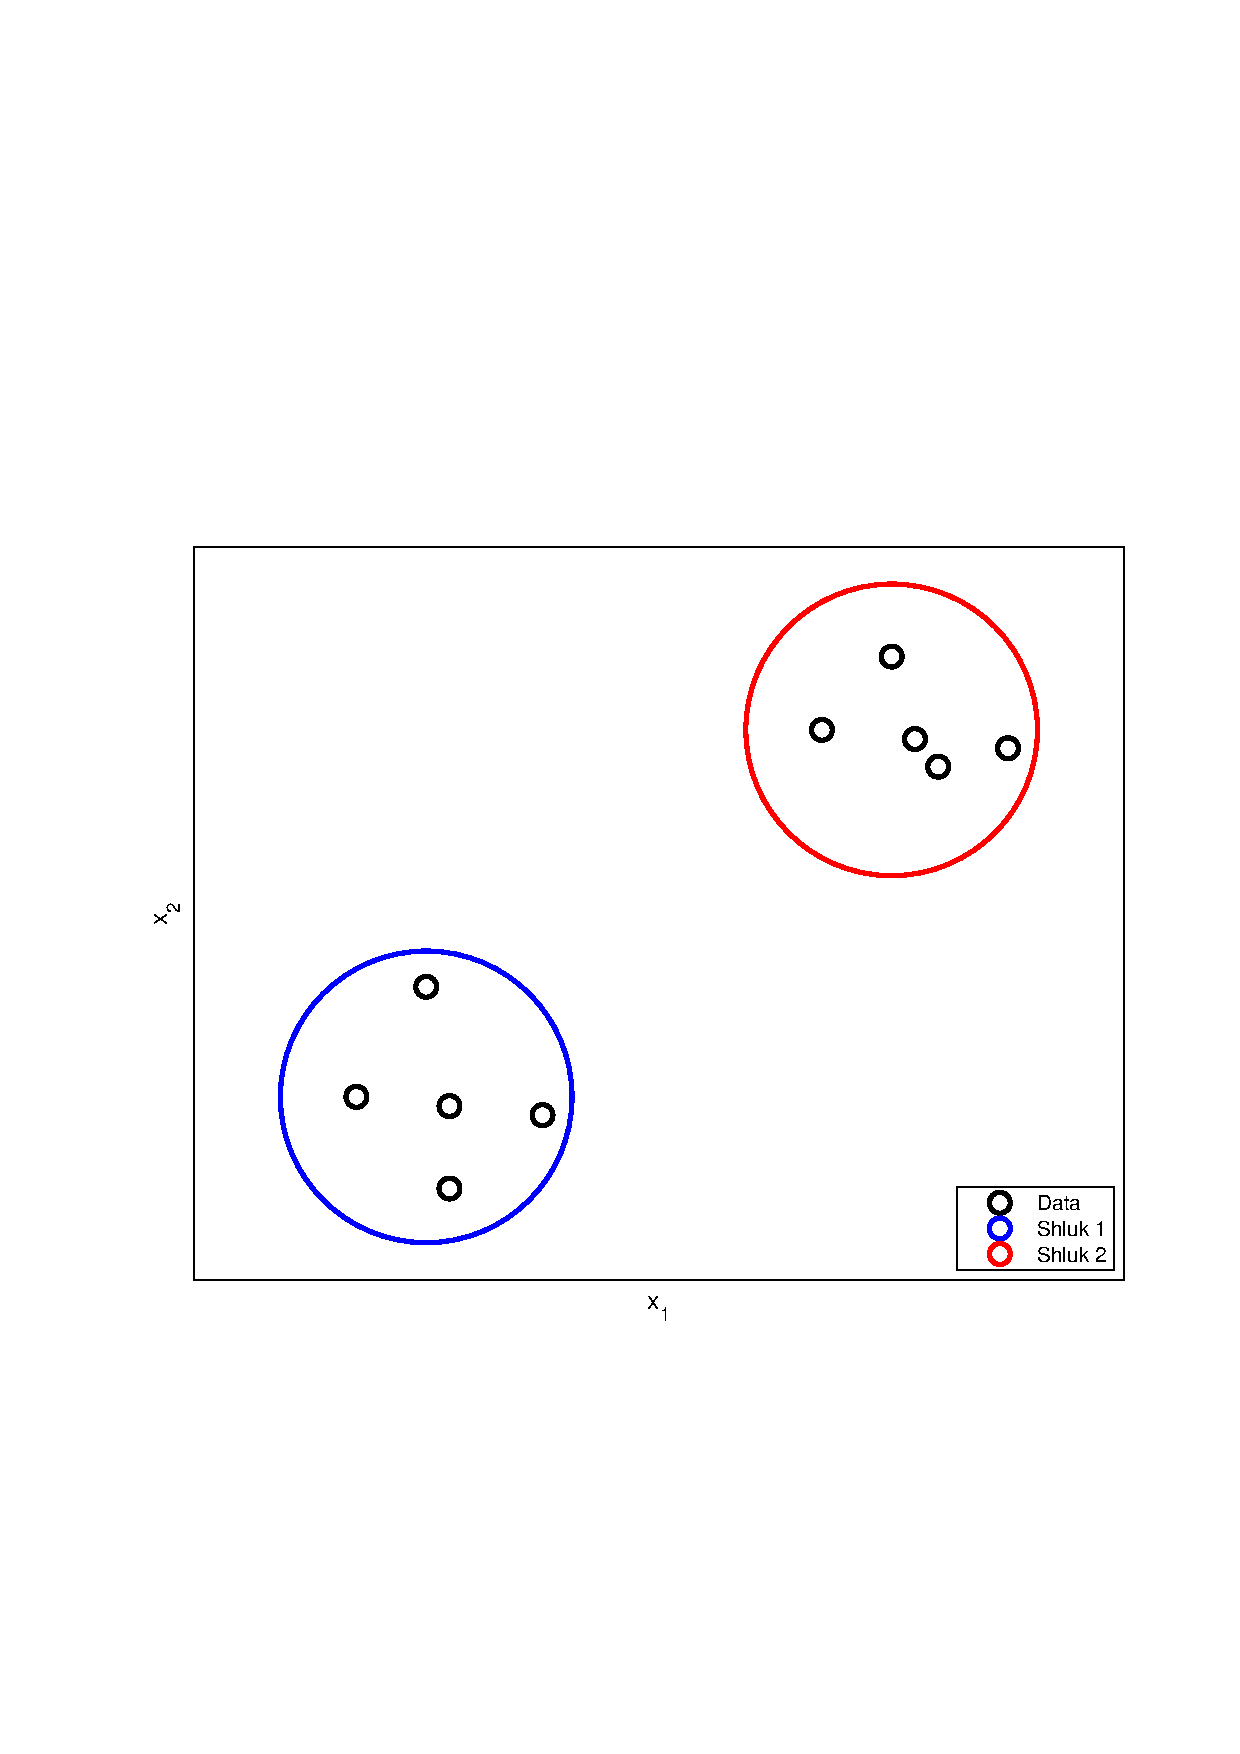
\includegraphics[width = \textwidth, trim = 2.5cm 7cm 2cm 9cm]{./Img/UnsupervizedLearning/Intro/unsupervized_circle.pdf}
  		\caption{Klasifikace do dvou tříd s naznačenými shluky - učení bez učitele.}
		\label{fig:unsupervized_circle}
	\end{minipage}%
\end{figure}}

\par{Příklad klasifikace v~případě učení bez učitele je \textbf{shlukování} , kde se jednotlivé třídy nazývají \textbf{shluky}.}



\newpage






\section{K-Means}

\par{}
\newpage











\section{Cíl optimalizace}

\par{}
\newpage











\section{Náhodná inicializace}

\par{}
\newpage











\section{Volba počtu shluků}

\par{}
\newpage



















\chapter{Redukce dimenze}

\section{Analýza hlavních komponent}
\par{Principal Component Analysis, PCA}

\section{Linear discriminant analysis}
\par{Linear discriminant analysis, LDA}

\chapter{Ostatní}


\section{GMM}

\section{Jak postavit test}
\par{testovaci trenovaci a cross validation sada}

\section{Vyhodnocování úspěšnosti klasifikace}
\par{recall, precision a F1 skore}




\end{document}

